\documentclass[t]{beamer}

\usetheme{metropolis}

\usepackage{graphicx}
\usepackage{multirow}
\usepackage{pgfplots}
\usepackage{pgfplotstable}
\usepackage{subcaption}
\usepackage{tikz}
\usepackage{transparent}

\author{Esten H{\o}yland Leonardsen}
\institute[Life Science, UiO]{UiO:Life Science, University of Oslo}
\date{24.10.22}
\title{Detecting individual-level deviations in brain morphology in MCI with explainable AI}

\titlegraphic{
	\vspace*{6.8cm}
	\centering
    
\includegraphics[width=1.5cm]{data/uio.png}
}
% TIKZ PACKAGES
\usetikzlibrary{arrows.meta}
\usetikzlibrary{calc}
\usetikzlibrary{patterns}
\usetikzlibrary{positioning}
\usetikzlibrary{shapes}

% PGFPLOTS PACKAGES
\usepgfplotslibrary{fillbetween}
\usepgfplotslibrary{groupplots}

% COLOUR
\definecolor{cb-pink}{HTML}{eeafcf}
\definecolor{cb-orange}{HTML}{e59145}
\definecolor{cb-light-brown}{HTML}{baa066}
\definecolor{cb-blue}{HTML}{3594d6}
\definecolor{cb-green}{HTML}{4dac93}
\definecolor{cb-gray}{HTML}{3a5c7d}
\definecolor{cb-light-purple}{HTML}{b45899}
\definecolor{cb-red-purple}{HTML}{c71555}
\definecolor{cb-brown}{HTML}{840000}
\definecolor{cb-blue-purple}{HTML}{662fa2}

\colorlet{cases-default}{cb-red-purple}
\colorlet{controls-default}{cb-blue}

\begin{document}

	\newcommand{\N}{1}

	\definecolor{outercolor}{RGB}{128, 128, 128}
	\newcommand{\nodesize}{11pt}
	\newcommand{\hsep}{28pt}
	\newcommand{\vsep}{14pt}

	\newcommand{\arrowwidth}{0.05cm}
	\newcommand{\innerarrow}{{Latex[length=0.1cm, width=0.15cm]}}
	\newcommand{\outerarrow}{{Latex[length=0.2cm, width=0.3cm]}}

	\def\plotwidth{11.68}

	\definecolor{outercolor}{RGB}{128, 128, 128}
	\colorlet{train-fill}{cb-green}

	\begin{frame} % Titlepage
		\titlepage
	\end{frame}

	\begin{frame}{Layerwise Relevance Propagation} % Forward pass
		\vfill
		\centering
		\begin{tikzpicture}
			\newcommand{\mrilocation}[1]{($(0, -2.2)$)}
			\newcommand{\modellocation}[1]{($ (4.5, -2.2) + ####1 $)}

			\colorlet{predict-fill}{cb-blue}

			\node[inner sep=0pt, outer sep=0pt,draw=black] (input) at \mrilocation{(0, 0)} {
				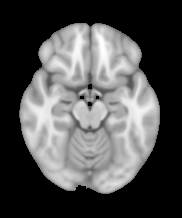
\includegraphics[width=1.2cm]{data/slice.png}
			};

			\node[circle, inner sep=0pt, fill=none, outer sep=0pt, line width=0pt, draw=none] (n00) at \modellocation{(-3 * \hsep, 0)} {};

			\node[circle, minimum size=\nodesize, inner sep=0pt, fill=predict-fill!85, outer sep=0pt, line width=0pt, draw=predict-fill!85] (n10) at \modellocation{(-2 * \hsep, 2 * \vsep)} {};
			\node[circle, minimum size=\nodesize, inner sep=0pt, fill=predict-fill, outer sep=0pt, line width=0pt, draw=predict-fill] (n11) at \modellocation{(-2 * \hsep, 1 * \vsep)} {};
			\node[circle, minimum size=\nodesize, inner sep=0pt, fill=predict-fill!75, outer sep=0pt, line width=0pt, draw=predict-fill!75] (n12) at \modellocation{(-2 * \hsep, 0)} {};
			\node[circle, minimum size=\nodesize, inner sep=0pt, fill=predict-fill!15, outer sep=0pt, line width=0pt, draw=predict-fill!15] (n13) at \modellocation{(-2 * \hsep, -1 * \vsep)} {};
			\node[circle, minimum size=\nodesize, inner sep=0pt, fill=predict-fill!50, outer sep=0pt, line width=0pt, draw=predict-fill!50] (n14) at \modellocation{(-2 * \hsep, -2 * \vsep)} {};

			\node[circle, minimum size=\nodesize, inner sep=0pt, fill=predict-fill!15, outer sep=0pt, line width=0pt, draw=predict-fill!15] (n20) at \modellocation{(-1 * \hsep, 1.5 * \vsep)} {};
			\node[circle, minimum size=\nodesize, inner sep=0pt, fill=predict-fill!65, outer sep=0pt, line width=0pt, draw=predict-fill!65] (n21) at \modellocation{(-1 * \hsep, 0.5 * \vsep)} {};
			\node[circle, minimum size=\nodesize, inner sep=0pt, fill=predict-fill!90, outer sep=0pt, line width=0pt, draw=predict-fill!90] (n22) at \modellocation{(-1 * \hsep, -0.5 * \vsep)} {};
			\node[circle, minimum size=\nodesize, inner sep=0pt, fill=predict-fill!40, outer sep=0pt, line width=0pt, draw=predict-fill!40] (n23) at \modellocation{(-1 * \hsep, -1.5 * \vsep)} {};

			\node[circle, minimum size=\nodesize, inner sep=0pt, fill=predict-fill!80, outer sep=0pt, line width=0pt, draw=predict-fill!80] (n30) at \modellocation{(0 * \hsep, 1.5 * \vsep)} {};
			\node[circle, minimum size=\nodesize, inner sep=0pt, fill=predict-fill!55, outer sep=0pt, line width=0pt, draw=predict-fill!55] (n31) at \modellocation{(0 * \hsep, 0.5 * \vsep)} {};
			\node[circle, minimum size=\nodesize, inner sep=0pt, fill=predict-fill!15, outer sep=0pt, line width=0pt, draw=predict-fill!15] (n32) at \modellocation{(0 * \hsep, -0.5 * \vsep)} {};
			\node[circle, minimum size=\nodesize, inner sep=0pt, fill=predict-fill!75, outer sep=0pt, line width=0pt, draw=predict-fill!75] (n33) at \modellocation{(0 * \hsep, -1.5 * \vsep)} {};

			\node[circle, minimum size=\nodesize, inner sep=0pt, fill=predict-fill, outer sep=0pt, line width=0pt, draw=predict-fill] (n40) at \modellocation{(1 * \hsep, 1*\vsep)} {};
			\node[circle, minimum size=\nodesize, inner sep=0pt, fill=predict-fill!20, outer sep=0pt, line width=0pt, draw=predict-fill!20] (n41) at \modellocation{(1 * \hsep, 0*\vsep)} {};
			\node[circle, minimum size=\nodesize, inner sep=0pt, fill=predict-fill!15, outer sep=0pt, line width=0pt, draw=predict-fill!15] (n42) at \modellocation{(1 * \hsep, -1*\vsep)} {};

			\node[circle, minimum size=\nodesize, inner sep=0pt, fill=predict-fill!75, outer sep=0pt, line width=0pt, draw=predict-fill!75] (n50) at \modellocation{(2 * \hsep, 1*\vsep)} {};
			\node[circle, minimum size=\nodesize, inner sep=0pt, fill=predict-fill!35, outer sep=0pt, line width=0pt, draw=predict-fill!35] (n51) at \modellocation{(2 * \hsep, 0*\vsep)} {};
			\node[circle, minimum size=\nodesize, inner sep=0pt, fill=predict-fill!65, outer sep=0pt, line width=0pt, draw=predict-fill!65] (n52) at \modellocation{(2 * \hsep, -1*\vsep)} {};

			\node[circle, minimum size=\nodesize, inner sep=0pt, fill=predict-fill!85, outer sep=0pt, line width=0pt, draw=predict-fill!85] (output) at \modellocation{(3 * \hsep, 0)} {};

			\node[] (diagnosis) at (9.3, -2.2) {\scriptsize{prediction}};

			\draw[
				color=predict-fill!85,
				-\innerarrow,
				line width=\arrowwidth
			] (n00) to [out=20,in=200] (n10) {};
			\draw[
				color=predict-fill,
				-\innerarrow,
				line width=\arrowwidth
			] (n00) to [out=10,in=190] (n11) {};
			\draw[
				color=predict-fill!75,
				-\innerarrow,
				line width=\arrowwidth
			] (n00) to [out=0,in=180] (n12) {};
			\draw[
				color=predict-fill!15,
				-\innerarrow,
				line width=\arrowwidth
			] (n00) to [out=-10,in=170] (n13) {};
			\draw[
				color=predict-fill!50,
				-\innerarrow,
				line width=\arrowwidth
			] (n00) to [out=-20,in=160] (n14) {};

			\draw[
				color=predict-fill!75,
				-\innerarrow,
				line width=\arrowwidth
			] (n10) to [out=-5,in=175] (n20) {};
			\draw[
				color=predict-fill!50,
				-\innerarrow,
				line width=\arrowwidth
			] (n10) to [out=-15,in=165] (n21) {};
			\draw[
				color=predict-fill!55,
				-\innerarrow,
				line width=\arrowwidth
			] (n10) to [out=-25,in=155] (n22) {};
			\draw[
				color=predict-fill!85,
				-\innerarrow,
				line width=\arrowwidth
			] (n10) to [out=-35,in=145] (n23) {};

			\draw[
				color=predict-fill!45,
				-\innerarrow,
				line width=\arrowwidth
			] (n11) to [out=5,in=185] (n20) {};
			\draw[
				color=predict-fill!50,
				-\innerarrow,
				line width=\arrowwidth
			] (n11) to [out=-5,in=175] (n21) {};
			\draw[
				color=predict-fill,
				-\innerarrow,
				line width=\arrowwidth
			] (n11) to [out=-15,in=165] (n22) {};
			\draw[
				color=predict-fill!15,
				-\innerarrow,
				line width=\arrowwidth
			] (n11) to [out=-25,in=155] (n23) {};

			\draw[
				color=predict-fill!35,
				-\innerarrow,
				line width=\arrowwidth
			] (n12) to [out=15,in=195] (n20) {};
			\draw[
				color=predict-fill!90,
				-\innerarrow,
				line width=\arrowwidth
			] (n12) to [out=5,in=185] (n21) {};
			\draw[
				color=predict-fill!80,
				-\innerarrow,
				line width=\arrowwidth
			] (n12) to [out=-5,in=175] (n22) {};
			\draw[
				color=predict-fill!20,
				-\innerarrow,
				line width=\arrowwidth
			] (n12) to [out=-15,in=165] (n23) {};

			\draw[
				color=predict-fill!55,
				-\innerarrow,
				line width=\arrowwidth
			] (n13) to [out=25,in=205] (n20) {};
			\draw[
				color=predict-fill!65,
				-\innerarrow,
				line width=\arrowwidth
			] (n13) to [out=15,in=195] (n21) {};
			\draw[
				color=predict-fill!35,
				-\innerarrow,
				line width=\arrowwidth
			] (n13) to [out=5,in=185] (n22) {};
			\draw[
				color=predict-fill!45,
				-\innerarrow,
				line width=\arrowwidth
			] (n13) to [out=-5,in=175] (n23) {};

			\draw[
				color=predict-fill!10,
				-\innerarrow,
				line width=\arrowwidth
			] (n14) to [out=35,in=215] (n20) {};
			\draw[
				color=predict-fill!90,
				-\innerarrow,
				line width=\arrowwidth
			] (n14) to [out=25,in=205] (n21) {};
			\draw[
				color=predict-fill!80,
				-\innerarrow,
				line width=\arrowwidth
			] (n14) to [out=15,in=195] (n22) {};
			\draw[
				color=predict-fill!35,
				-\innerarrow,
				line width=\arrowwidth
			] (n14) to [out=5,in=185] (n23) {};

			\draw[
				color=predict-fill!75,
				-\innerarrow,
				line width=\arrowwidth
			] (n20) to [out=0,in=180] (n30) {};
			\draw[
				color=predict-fill!50,
				-\innerarrow,
				line width=\arrowwidth
			] (n20) to [out=-10,in=170] (n31) {};
			\draw[
				color=predict-fill!85,
				-\innerarrow,
				line width=\arrowwidth
			] (n20) to [out=-20,in=160] (n32) {};
			\draw[
				color=predict-fill!45,
				-\innerarrow,
				line width=\arrowwidth
			] (n20) to [out=-30,in=150] (n33) {};

			\draw[
				color=predict-fill!20,
				-\innerarrow,
				line width=\arrowwidth
			] (n21) to [out=10,in=190] (n30) {};
			\draw[
				color=predict-fill!35,
				-\innerarrow,
				line width=\arrowwidth
			] (n21) to [out=0,in=180] (n31) {};
			\draw[
				color=predict-fill!15,
				-\innerarrow,
				line width=\arrowwidth
			] (n21) to [out=-10,in=170] (n32) {};
			\draw[
				color=predict-fill!90,
				-\innerarrow,
				line width=\arrowwidth
			] (n21) to [out=-20,in=160] (n33) {};

			\draw[
				color=predict-fill!65,
				-\innerarrow,
				line width=\arrowwidth
			] (n22) to [out=20,in=200] (n30) {};
			\draw[
				color=predict-fill!20,
				-\innerarrow,
				line width=\arrowwidth
			] (n22) to [out=10,in=190] (n31) {};
			\draw[
				color=predict-fill!30,
				-\innerarrow,
				line width=\arrowwidth
			] (n22) to [out=0,in=180] (n32) {};
			\draw[
				color=predict-fill!40,
				-\innerarrow,
				line width=\arrowwidth
			] (n22) to [out=-10,in=170] (n33) {};

			\draw[
				color=predict-fill,
				-\innerarrow,
				line width=\arrowwidth
			] (n23) to [out=30,in=210] (n30) {};
			\draw[
				color=predict-fill!15,
				-\innerarrow,
				line width=\arrowwidth
			] (n23) to [out=20,in=200] (n31) {};
			\draw[
				color=predict-fill!75,
				-\innerarrow,
				line width=\arrowwidth
			] (n23) to [out=10,in=190] (n32) {};
			\draw[
				color=predict-fill!35,
				-\innerarrow,
				line width=\arrowwidth
			] (n23) to [out=0,in=180] (n33) {};

			\draw[
				color=predict-fill!70,
				-\innerarrow,
				line width=\arrowwidth
			] (n30) to [out=-5,in=175] (n40) {};
			\draw[
				color=predict-fill!80,
				-\innerarrow,
				line width=\arrowwidth
			] (n30) to [out=-15,in=165] (n41) {};
			\draw[
				color=predict-fill!20,
				-\innerarrow,
				line width=\arrowwidth
			] (n30) to [out=-25,in=155] (n42) {};

			\draw[
				color=predict-fill!60,
				-\innerarrow,
				line width=\arrowwidth
			] (n31) to [out=5,in=185] (n40) {};
			\draw[
				color=predict-fill!95,
				-\innerarrow,
				line width=\arrowwidth
			] (n31) to [out=-5,in=175] (n41) {};
			\draw[
				color=predict-fill!35,
				-\innerarrow,
				line width=\arrowwidth
			] (n31) to [out=-15,in=165] (n42) {};

			\draw[
				color=predict-fill!75,
				-\innerarrow,
				line width=\arrowwidth
			] (n32) to [out=15,in=195] (n40) {};
			\draw[
				color=predict-fill!20,
				-\innerarrow,
				line width=\arrowwidth
			] (n32) to [out=5,in=185] (n41) {};
			\draw[
				color=predict-fill!15,
				-\innerarrow,
				line width=\arrowwidth
			] (n32) to [out=-5,in=175] (n42) {};

			\draw[
				color=predict-fill!40,
				-\innerarrow,
				line width=\arrowwidth
			] (n33) to [out=25,in=205] (n40) {};
			\draw[
				color=predict-fill!80,
				-\innerarrow,
				line width=\arrowwidth
			] (n33) to [out=15,in=195] (n41) {};
			\draw[
				color=predict-fill!50,
				-\innerarrow,
				line width=\arrowwidth
			] (n33) to [out=5,in=185] (n42) {};

			\draw[
				color=predict-fill!25,
				-\innerarrow,
				line width=\arrowwidth
			] (n40) to [out=0,in=180] (n50) {};
			\draw[
				color=predict-fill!50,
				-\innerarrow,
				line width=\arrowwidth
			] (n40) to [out=-10,in=170] (n51) {};
			\draw[
				color=predict-fill!45,
				-\innerarrow,
				line width=\arrowwidth
			] (n40) to [out=-20,in=160] (n52) {};

			\draw[
				color=predict-fill!90,
				-\innerarrow,
				line width=\arrowwidth
			] (n41) to [out=10,in=190] (n50) {};
			\draw[
				color=predict-fill!10,
				-\innerarrow,
				line width=\arrowwidth
			] (n41) to [out=0,in=180] (n51) {};
			\draw[
				color=predict-fill!75,
				-\innerarrow,
				line width=\arrowwidth
			] (n41) to [out=-10,in=170] (n52) {};

			\draw[
				color=predict-fill!60,
				-\innerarrow,
				line width=\arrowwidth
			] (n42) to [out=20,in=200] (n50) {};
			\draw[
				color=predict-fill!25,
				-\innerarrow,
				line width=\arrowwidth
			] (n42) to [out=10,in=190] (n51) {};
			\draw[
				color=predict-fill!15,
				-\innerarrow,
				line width=\arrowwidth
			] (n42) to [out=0,in=180] (n52) {};

			\draw[
				color=predict-fill!95,
				-\innerarrow,
				line width=\arrowwidth
			] (n50) to [out=-10,in=170] (output) {};
			\draw[
				color=predict-fill!25,
				-\innerarrow,
				line width=\arrowwidth
			] (n51) to [out=0,in=180] (output) {};
			\draw[
				color=predict-fill!50,
				-\innerarrow,
				line width=\arrowwidth
			] (n52) to [out=10,in=190] (output) {};

			\draw[black] (n00.center) --
						 ($ (n00) + (0, 2*\vsep+0.5*\nodesize+2pt) $) --
						 ($ (n00) + (6*\hsep+0.5*\nodesize+2pt, 2*\vsep+0.5*\nodesize+2pt) $) --
						 ($ (n00) + (6*\hsep+0.5*\nodesize+2pt, -2*\vsep-0.5*\nodesize-2pt) $) --
						 ($ (n00) + (0, -2*\vsep-0.5*\nodesize-2pt) $) -- (n00.center);

			\node[text depth=0] at ($ (n30) + (0, \vsep+0.5*\nodesize) $) {\footnotesize{Prediction model}};

			\draw[
				color=outercolor,
				-\outerarrow,
				line width=0.1cm
			] (input) to [out=0,in=180] (n00) {};
			\draw[
				color=outercolor,
				-\outerarrow,
				line width=0.1cm
			] (output) to [out=0,in=180] (diagnosis) {};

			\node[] at (2.8, -4.3) {\footnotesize{$n_{i,j}=\sum\limits_k n_{i-1,k}w_{k,j}$}};
		\end{tikzpicture}
		\vfill
	\end{frame}

	\begin{frame}{Layerwise Relevance Propagation} % Backward pass
		\vfill
		\centering
		\begin{tikzpicture}
			\newcommand{\mrilocation}[1]{($(0, -2.2)$)}
			\newcommand{\lrplocation}[1]{($ (4.5, -2.2) + ####1 $)}

			\node[inner sep=0pt, outer sep=0pt, minimum width=1.2cm] (input) at \mrilocation{(0, 0)} {};

			\node[circle, inner sep=0pt, fill=none, outer sep=0pt, line width=0pt, draw=none] (n00) at \lrplocation{(-3 * \hsep, 0)} {};

			\node[circle, minimum size=\nodesize, inner sep=0pt, fill={rgb:black,5;orange,1}, outer sep=0pt, line width=0pt, draw={rgb:black,5;orange,1}] (n10) at \lrplocation{(-2 * \hsep, 2 * \vsep)} {};
			\node[circle, minimum size=\nodesize, inner sep=0pt, fill={rgb:black,3;red,1}, outer sep=0pt, line width=0pt, draw={rgb:black,3;red,1}] (n11) at \lrplocation{(-2 * \hsep, 1 * \vsep)} {};
			\node[circle, minimum size=\nodesize, inner sep=0pt, fill=yellow, outer sep=0pt, line width=0pt, draw=yellow] (n12) at \lrplocation{(-2 * \hsep, 0)} {};
			\node[circle, minimum size=\nodesize, inner sep=0pt, fill=black, outer sep=0pt, line width=0pt, draw=black] (n13) at \lrplocation{(-2 * \hsep, -1 * \vsep)} {};
			\node[circle, minimum size=\nodesize, inner sep=0pt, fill=red, outer sep=0pt, line width=0pt, draw=red] (n14) at \lrplocation{(-2 * \hsep, -2 * \vsep)} {};

			\node[circle, minimum size=\nodesize, inner sep=0pt, fill={rgb:black,5;white,2;orange,1}, outer sep=0pt, line width=0pt, draw={rgb:black,5;white,2;orange,1}] (n20) at \lrplocation{(-1 * \hsep, 1.5 * \vsep)} {};
			\node[circle, minimum size=\nodesize, inner sep=0pt, fill={rgb:red,10;yellow,6}, outer sep=0pt, line width=0pt, draw={rgb:red,10;yellow,4}] (n21) at \lrplocation{(-1 * \hsep, 0.5 * \vsep)} {};
			\node[circle, minimum size=\nodesize, inner sep=0pt, fill={rgb:red,10;yellow,1}, outer sep=0pt, line width=0pt, draw={rgb:red,10;yellow,1}] (n22) at \lrplocation{(-1 * \hsep, -0.5 * \vsep)} {};
			\node[circle, minimum size=\nodesize, inner sep=0pt, fill={rgb:black,10;red,2}, outer sep=0pt, line width=0pt, draw={rgb:black,10;red,2}] (n23) at \lrplocation{(-1 * \hsep, -1.5 * \vsep)} {};

			\node[circle, minimum size=\nodesize, inner sep=0pt, fill={rgb:red,3;orange,2}, outer sep=0pt, line width=0pt, draw={rgb:red,3;orange,1}] (n30) at \lrplocation{(0 * \hsep, 1.5 * \vsep)} {};
			\node[circle, minimum size=\nodesize, inner sep=0pt, fill={rgb:yellow,3;orange,1}, outer sep=0pt, line width=0pt, draw={rgb:yellow,3;orange,1}] (n31) at \lrplocation{(0 * \hsep, 0.5 * \vsep)} {};
			\node[circle, minimum size=\nodesize, inner sep=0pt, fill={rgb:black,10;white,5;red,1}, outer sep=0pt, line width=0pt, draw={rgb:black,10;white,5;red,1}] (n32) at \lrplocation{(0 * \hsep, -0.5 * \vsep)} {};
			\node[circle, minimum size=\nodesize, inner sep=0pt, fill={rgb:gray,5;red,1}, outer sep=0pt, line width=0pt, draw={rgb:gray,5;red,1}] (n33) at \lrplocation{(0 * \hsep, -1.5 * \vsep)} {};

			\node[circle, minimum size=\nodesize, inner sep=0pt, fill={rgb:yellow,10;orange,1}, outer sep=0pt, line width=0pt, draw={rgb:yellow,10;orange,1}] (n40) at \lrplocation{(1 * \hsep, 1*\vsep)} {};
			\node[circle, minimum size=\nodesize, inner sep=0pt, fill={rgb:red,1}, outer sep=0pt, line width=0pt, draw={rgb:red,1}] (n41) at \lrplocation{(1 * \hsep, 0*\vsep)} {};
			\node[circle, minimum size=\nodesize, inner sep=0pt, fill={rgb:black,10;white,15;red,2}, outer sep=0pt, line width=0pt, draw={rgb:black,10;white,15;red,2}] (n42) at \lrplocation{(1 * \hsep, -1*\vsep)} {};

			\node[circle, minimum size=\nodesize, inner sep=0pt, fill={rgb:red,5;black,1;yellow,2}, outer sep=0pt, line width=0pt, draw={rgb:red,5;black,1;yellow,2}] (n50) at \lrplocation{(2 * \hsep, 1*\vsep)} {};
			\node[circle, minimum size=\nodesize, inner sep=0pt, fill={rgb:gray,5;red,1}, outer sep=0pt, line width=0pt, draw={rgb:gray,5;red,1}] (n51) at \lrplocation{(2 * \hsep, 0*\vsep)} {};
			\node[circle, minimum size=\nodesize, inner sep=0pt, fill={rgb:yellow,5;orange,1}, outer sep=0pt, line width=0pt, draw={rgb:yellow,5;orange,1}] (n52) at \lrplocation{(2 * \hsep, -1*\vsep)} {};

			\node[circle, minimum size=\nodesize, inner sep=0pt, fill={rgb:orange,7;yellow,4;black,1}, outer sep=0pt, line width=0pt, draw={rgb:orange,7;yellow,4;black,1}] (n60) at \lrplocation{(3 * \hsep, 0)} {};

			\draw[
				color={rgb:black,5;orange,1},
				\innerarrow-,
				line width=\arrowwidth
			] (n00) to [out=20,in=200] (n10) {};
			\draw[
				color={rgb:black,3;red,1},
				\innerarrow-,
				line width=\arrowwidth
			] (n00) to [out=10,in=190] (n11) {};
			\draw[
				color=yellow,
				\innerarrow-,
				line width=\arrowwidth
			] (n00) to [out=0,in=180] (n12) {};
			\draw[
				color=black,
				\innerarrow-,
				line width=\arrowwidth
			] (n00) to [out=-10,in=170] (n13) {};
			\draw[
				color=red,
				\innerarrow-,
				line width=\arrowwidth
			] (n00) to [out=-20,in=160] (n14) {};

			\draw[
				color={rgb:black,5;white,1;orange,1},
				\innerarrow-,
				line width=\arrowwidth
			] (n10) to [out=-5,in=175] (n20) {};
			\draw[
				color={rgb:black,3;orange,1},
				\innerarrow-,
				line width=\arrowwidth
			] (n10) to [out=-15,in=165] (n21) {};
			\draw[
				color={rgb:black,4;red,2;yellow,1},
				\innerarrow-,
				line width=\arrowwidth
			] (n10) to [out=-25,in=155] (n22) {};
			\draw[
				color={rgb:black,3;red,1},
				\innerarrow-,
				line width=\arrowwidth
			] (n10) to [out=-35,in=145] (n23) {};

			\draw[
				color={rgb:black,10;orange,2},
				\innerarrow-,
				line width=\arrowwidth
			] (n11) to [out=5,in=185] (n20) {};
			\draw[
				color={rgb:black,3;orange,1},
				\innerarrow-,
				line width=\arrowwidth
			] (n11) to [out=-5,in=175] (n21) {};
			\draw[
				color={rgb:black,3;red,1},
				\innerarrow-,
				line width=\arrowwidth
			] (n11) to [out=-15,in=165] (n22) {};
			\draw[
				color={rgb:black,10;red,1},
				\innerarrow-,
				line width=\arrowwidth
			] (n11) to [out=-25,in=155] (n23) {};

			\draw[
				color={rgb:black,5;orange,3},
				\innerarrow-,
				line width=\arrowwidth
			] (n12) to [out=15,in=195] (n20) {};
			\draw[
				color={rgb:red,3;yellow,5},
				\innerarrow-,
				line width=\arrowwidth
			] (n12) to [out=5,in=185] (n21) {};
			\draw[
				color={rgb:red,5;yellow,3},
				\innerarrow-,
				line width=\arrowwidth
			] (n12) to [out=-5,in=175] (n22) {};
			\draw[
				color={rgb:black,5;orange,2},
				\innerarrow-,
				line width=\arrowwidth
			] (n12) to [out=-15,in=165] (n23) {};

			\draw[
				color={rgb:black,5;red,1},
				\innerarrow-,
				line width=\arrowwidth
			] (n13) to [out=25,in=205] (n20) {};
			\draw[
				color={rgb:black,5;orange,2},
				\innerarrow-,
				line width=\arrowwidth
			] (n13) to [out=15,in=195] (n21) {};
			\draw[
				color={rgb:black,5;red,3},
				\innerarrow-,
				line width=\arrowwidth
			] (n13) to [out=5,in=185] (n22) {};
			\draw[
				color=black,
				\innerarrow-,
				line width=\arrowwidth
			] (n13) to [out=-5,in=175] (n23) {};

			\draw[
				color={rgb:black,5;orange,2},
				\innerarrow-,
				line width=\arrowwidth
			] (n14) to [out=35,in=215] (n20) {};
			\draw[
				color={rgb:red,3;orange,1},
				\innerarrow-,
				line width=\arrowwidth
			] (n14) to [out=25,in=205] (n21) {};
			\draw[
				color={rgb:red,5;yellow,2},
				\innerarrow-,
				line width=\arrowwidth
			] (n14) to [out=15,in=195] (n22) {};
			\draw[
				color={rgb:black,5;red,3},
				\innerarrow-,
				line width=\arrowwidth
			] (n14) to [out=5,in=185] (n23) {};

			\draw[
				color={rgb:black,1;red,1},
				\innerarrow-,
				line width=\arrowwidth
			] (n20) to [out=0,in=180] (n30) {};
			\draw[
				color={rgb:black,3;orange,1},
				\innerarrow-,
				line width=\arrowwidth
			] (n20) to [out=-10,in=170] (n31) {};
			\draw[
				color={rgb:black,10;red,1},
				\innerarrow-,
				line width=\arrowwidth
			] (n20) to [out=-20,in=160] (n32) {};
			\draw[
				color={rgb:black,5;red,1},
				\innerarrow-,
				line width=\arrowwidth
			] (n20) to [out=-30,in=150] (n33) {};

			\draw[
				color={rgb:orange,5;red,2},
				\innerarrow-,
				line width=\arrowwidth
			] (n21) to [out=10,in=190] (n30) {};
			\draw[
				color={rgb:yellow,10;orange,4},
				\innerarrow-,
				line width=\arrowwidth
			] (n21) to [out=0,in=180] (n31) {};
			\draw[
				color={rgb:black,2;red,1},
				\innerarrow-,
				line width=\arrowwidth
			] (n21) to [out=-10,in=170] (n32) {};
			\draw[
				color={rgb:black,1;orange,2;red,1},
				\innerarrow-,
				line width=\arrowwidth
			] (n21) to [out=-20,in=160] (n33) {};

			\draw[
				color={rgb:red,2;orange,1},
				\innerarrow-,
				line width=\arrowwidth
			] (n22) to [out=20,in=200] (n30) {};
			\draw[
				color={rgb:yellow,2;orange,1},
				\innerarrow-,
				line width=\arrowwidth
			] (n22) to [out=10,in=190] (n31) {};
			\draw[
				color={rgb:black,2;red,2},
				\innerarrow-,
				line width=\arrowwidth
			] (n22) to [out=0,in=180] (n32) {};
			\draw[
				color={rgb:black,2;orange,1},
				\innerarrow-,
				line width=\arrowwidth
			] (n22) to [out=-10,in=170] (n33) {};

			\draw[
				color={rgb:black,4;red,2},
				\innerarrow-,
				line width=\arrowwidth
			] (n23) to [out=30,in=210] (n30) {};
			\draw[
				color={rgb:orange,2;black,1},
				\innerarrow-,
				line width=\arrowwidth
			] (n23) to [out=20,in=200] (n31) {};
			\draw[
				color={rgb:black,5;orange,1},
				\innerarrow-,
				line width=\arrowwidth
			] (n23) to [out=10,in=190] (n32) {};
			\draw[
				color={rgb:black,5;red,2},
				\innerarrow-,
				line width=\arrowwidth
			] (n23) to [out=0,in=180] (n33) {};

			\draw[
				color={rgb:orange,3;red,1},
				\innerarrow-,
				line width=\arrowwidth
			] (n30) to [out=-5,in=175] (n40) {};
			\draw[
				color={rgb:gray,1;orange,1;red,2},
				\innerarrow-,
				line width=\arrowwidth
			] (n30) to [out=-15,in=165] (n41) {};
			\draw[
				color={rgb:orange,2;black,2;white,1},
				\innerarrow-,
				line width=\arrowwidth
			] (n30) to [out=-25,in=155] (n42) {};

			\draw[
				color={rgb:yellow,5;orange,1},
				\innerarrow-,
				line width=\arrowwidth
			] (n31) to [out=5,in=185] (n40) {};
			\draw[
				color={rgb:red,3;orange,1},
				\innerarrow-,
				line width=\arrowwidth
			] (n31) to [out=-5,in=175] (n41) {};
			\draw[
				color={rgb:gray,1;red,2},
				\innerarrow-,
				line width=\arrowwidth
			] (n31) to [out=-15,in=165] (n42) {};

			\draw[
				color={rgb:gray,3;orange,1},
				\innerarrow-,
				line width=\arrowwidth
			] (n32) to [out=15,in=195] (n40) {};
			\draw[
				color={rgb:gray,1;red,1},
				\innerarrow-,
				line width=\arrowwidth
			] (n32) to [out=5,in=185] (n41) {};
			\draw[
				color={rgb:gray,1},
				\innerarrow-,
				line width=\arrowwidth
			] (n32) to [out=-5,in=175] (n42) {};

			\draw[
				color={rgb:gray,2;orange,3},
				\innerarrow-,
				line width=\arrowwidth
			] (n33) to [out=25,in=205] (n40) {};
			\draw[
				color={rgb:gray,1;orange,1},
				\innerarrow-,
				line width=\arrowwidth
			] (n33) to [out=15,in=195] (n41) {};
			\draw[
				color={rgb:gray,3;red,1},
				\innerarrow-,
				line width=\arrowwidth
			] (n33) to [out=5,in=185] (n42) {};

			\draw[
				color={rgb:red,3;yellow,1},
				\innerarrow-,
				line width=\arrowwidth
			] (n40) to [out=0,in=180] (n50) {};
			\draw[
				color={rgb:gray,2;orange,1},
				\innerarrow-,
				line width=\arrowwidth
			] (n40) to [out=-10,in=170] (n51) {};
			\draw[
				color={rgb:yellow,10;orange,1},
				\innerarrow-,
				line width=\arrowwidth
			] (n40) to [out=-20,in=160] (n52) {};

			\draw[
				color={rgb:red,5;black,1;yellow,2},
				\innerarrow-,
				line width=\arrowwidth
			] (n41) to [out=10,in=190] (n50) {};
			\draw[
				color={rgb:gray,7;orange,3},
				\innerarrow-,
				line width=\arrowwidth
			] (n41) to [out=0,in=180] (n51) {};
			\draw[
				color={rgb:yellow,1;orange,2},
				\innerarrow-,
				line width=\arrowwidth
			] (n41) to [out=-10,in=170] (n52) {};

			\draw[
				color={rgb:gray,7;orange,2},
				\innerarrow-,
				line width=\arrowwidth
			] (n42) to [out=20,in=200] (n50) {};
			\draw[
				color={rgb:gray,5;red,1},
				\innerarrow-,
				line width=\arrowwidth
			] (n42) to [out=10,in=190] (n51) {};
			\draw[
				color={rgb:gray,5;red,1;black,2},
				\innerarrow-,
				line width=\arrowwidth
			] (n42) to [out=0,in=180] (n52) {};

			\draw[
				color={rgb:red,5;black,1;yellow,2},
				\innerarrow-,
				line width=\arrowwidth
			] (n50) to [out=-10,in=170] (n60) {};
			\draw[
				color={rgb:gray,5;red,1},
				\innerarrow-,
				line width=\arrowwidth
			] (n51) to [out=0,in=180] (n60) {};
			\draw[
				color={rgb:yellow,5;orange,1},
				\innerarrow-,
				line width=\arrowwidth
			] (n52) to [out=10,in=190] (n60) {};

			\draw[black] (n00.center) --
						($ (n00) + (0, 2*\vsep+0.5*\nodesize+2pt) $) --
						($ (n00) + (6*\hsep+0.5*\nodesize+2pt, 2*\vsep+0.5*\nodesize+2pt) $) --
						($ (n00) + (6*\hsep+0.5*\nodesize+2pt, -2*\vsep-0.5*\nodesize-2pt) $) --
						($ (n00) + (0, -2*\vsep-0.5*\nodesize-2pt) $) -- (n00.center);

			\node[text depth=0] at ($ (n30) + (0, \vsep+0.5*\nodesize) $) {\footnotesize{Layerwise Relevance Propagation}};

			\node[] (diagnosis) at (9.3, -2.2) {\scriptsize{prediction}};


			\draw[
				color=outercolor,
				\outerarrow-,
				line width=0.1cm
			] (output) to [out=0,in=180] (diagnosis) {};

			\node[] at (2.8, -4.3) {\textcolor{black!30}{\footnotesize{$n_{i,j}=\sum\limits_k n_{i-1,k}w_{k,j}$}}};
			\node[] at (6.2, -4.3) {\footnotesize{$R_{i,j}=\sum\limits_k \frac{a_jw_{j,k}}{\sum\limits_l a_lw_{l,k}}R_{i+1,k}$}};

		\end{tikzpicture}
		\vfill
	\end{frame}

	\begin{frame}{Layerwise Relevance Propagation} % Heatmap
		\vfill
		\centering
		\begin{tikzpicture}
			\newcommand{\mrilocation}[1]{($(0, -2.2)$)}
			\newcommand{\lrplocation}[1]{($ (4.5, -2.2) + ####1 $)}

			\node[inner sep=0pt, outer sep=0pt, minimum width=1.2cm] (input) at \mrilocation{(0, 0)} {
				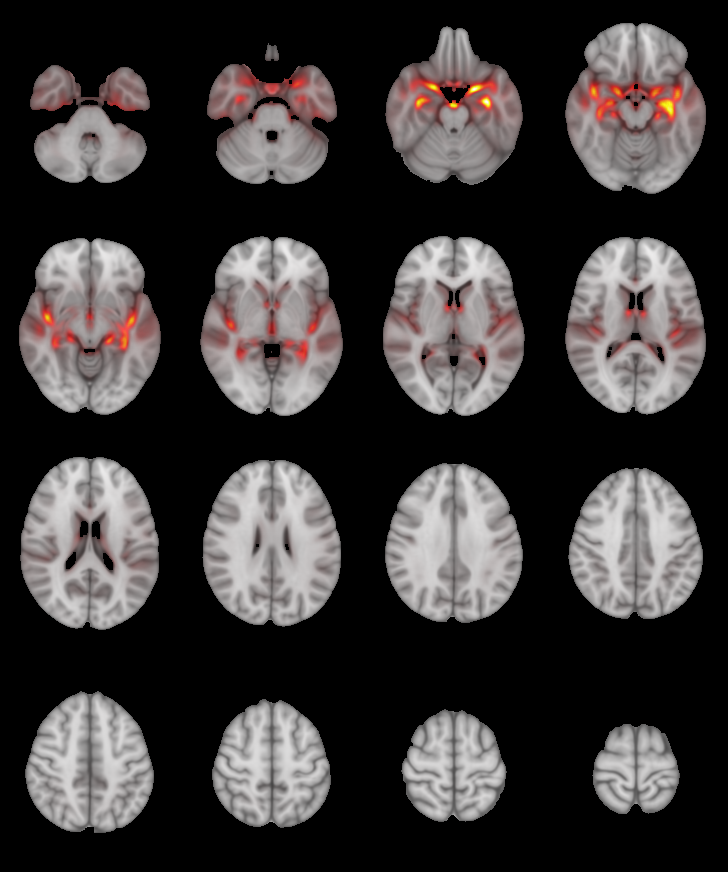
\includegraphics[
					width=1.2cm,
					clip=true,
					trim = 192mm 232mm 0mm 0mm
				]{data/dementia_average.png}
			};

			\node[circle, inner sep=0pt, fill=none, outer sep=0pt, line width=0pt, draw=none] (n00) at \lrplocation{(-3 * \hsep, 0)} {};

			\node[circle, minimum size=\nodesize, inner sep=0pt, fill={rgb:black,5;orange,1}, outer sep=0pt, line width=0pt, draw={rgb:black,5;orange,1}] (n10) at \lrplocation{(-2 * \hsep, 2 * \vsep)} {};
			\node[circle, minimum size=\nodesize, inner sep=0pt, fill={rgb:black,3;red,1}, outer sep=0pt, line width=0pt, draw={rgb:black,3;red,1}] (n11) at \lrplocation{(-2 * \hsep, 1 * \vsep)} {};
			\node[circle, minimum size=\nodesize, inner sep=0pt, fill=yellow, outer sep=0pt, line width=0pt, draw=yellow] (n12) at \lrplocation{(-2 * \hsep, 0)} {};
			\node[circle, minimum size=\nodesize, inner sep=0pt, fill=black, outer sep=0pt, line width=0pt, draw=black] (n13) at \lrplocation{(-2 * \hsep, -1 * \vsep)} {};
			\node[circle, minimum size=\nodesize, inner sep=0pt, fill=red, outer sep=0pt, line width=0pt, draw=red] (n14) at \lrplocation{(-2 * \hsep, -2 * \vsep)} {};

			\node[circle, minimum size=\nodesize, inner sep=0pt, fill={rgb:black,5;white,2;orange,1}, outer sep=0pt, line width=0pt, draw={rgb:black,5;white,2;orange,1}] (n20) at \lrplocation{(-1 * \hsep, 1.5 * \vsep)} {};
			\node[circle, minimum size=\nodesize, inner sep=0pt, fill={rgb:red,10;yellow,6}, outer sep=0pt, line width=0pt, draw={rgb:red,10;yellow,4}] (n21) at \lrplocation{(-1 * \hsep, 0.5 * \vsep)} {};
			\node[circle, minimum size=\nodesize, inner sep=0pt, fill={rgb:red,10;yellow,1}, outer sep=0pt, line width=0pt, draw={rgb:red,10;yellow,1}] (n22) at \lrplocation{(-1 * \hsep, -0.5 * \vsep)} {};
			\node[circle, minimum size=\nodesize, inner sep=0pt, fill={rgb:black,10;red,2}, outer sep=0pt, line width=0pt, draw={rgb:black,10;red,2}] (n23) at \lrplocation{(-1 * \hsep, -1.5 * \vsep)} {};

			\node[circle, minimum size=\nodesize, inner sep=0pt, fill={rgb:red,3;orange,2}, outer sep=0pt, line width=0pt, draw={rgb:red,3;orange,1}] (n30) at \lrplocation{(0 * \hsep, 1.5 * \vsep)} {};
			\node[circle, minimum size=\nodesize, inner sep=0pt, fill={rgb:yellow,3;orange,1}, outer sep=0pt, line width=0pt, draw={rgb:yellow,3;orange,1}] (n31) at \lrplocation{(0 * \hsep, 0.5 * \vsep)} {};
			\node[circle, minimum size=\nodesize, inner sep=0pt, fill={rgb:black,10;white,5;red,1}, outer sep=0pt, line width=0pt, draw={rgb:black,10;white,5;red,1}] (n32) at \lrplocation{(0 * \hsep, -0.5 * \vsep)} {};
			\node[circle, minimum size=\nodesize, inner sep=0pt, fill={rgb:gray,5;red,1}, outer sep=0pt, line width=0pt, draw={rgb:gray,5;red,1}] (n33) at \lrplocation{(0 * \hsep, -1.5 * \vsep)} {};

			\node[circle, minimum size=\nodesize, inner sep=0pt, fill={rgb:yellow,10;orange,1}, outer sep=0pt, line width=0pt, draw={rgb:yellow,10;orange,1}] (n40) at \lrplocation{(1 * \hsep, 1*\vsep)} {};
			\node[circle, minimum size=\nodesize, inner sep=0pt, fill={rgb:red,1}, outer sep=0pt, line width=0pt, draw={rgb:red,1}] (n41) at \lrplocation{(1 * \hsep, 0*\vsep)} {};
			\node[circle, minimum size=\nodesize, inner sep=0pt, fill={rgb:black,10;white,15;red,2}, outer sep=0pt, line width=0pt, draw={rgb:black,10;white,15;red,2}] (n42) at \lrplocation{(1 * \hsep, -1*\vsep)} {};

			\node[circle, minimum size=\nodesize, inner sep=0pt, fill={rgb:red,5;black,1;yellow,2}, outer sep=0pt, line width=0pt, draw={rgb:red,5;black,1;yellow,2}] (n50) at \lrplocation{(2 * \hsep, 1*\vsep)} {};
			\node[circle, minimum size=\nodesize, inner sep=0pt, fill={rgb:gray,5;red,1}, outer sep=0pt, line width=0pt, draw={rgb:gray,5;red,1}] (n51) at \lrplocation{(2 * \hsep, 0*\vsep)} {};
			\node[circle, minimum size=\nodesize, inner sep=0pt, fill={rgb:yellow,5;orange,1}, outer sep=0pt, line width=0pt, draw={rgb:yellow,5;orange,1}] (n52) at \lrplocation{(2 * \hsep, -1*\vsep)} {};

			\node[circle, minimum size=\nodesize, inner sep=0pt, fill={rgb:orange,7;yellow,4;black,1}, outer sep=0pt, line width=0pt, draw={rgb:orange,7;yellow,4;black,1}] (n60) at \lrplocation{(3 * \hsep, 0)} {};

			\draw[
				color={rgb:black,5;orange,1},
				\innerarrow-,
				line width=\arrowwidth
			] (n00) to [out=20,in=200] (n10) {};
			\draw[
				color={rgb:black,3;red,1},
				\innerarrow-,
				line width=\arrowwidth
			] (n00) to [out=10,in=190] (n11) {};
			\draw[
				color=yellow,
				\innerarrow-,
				line width=\arrowwidth
			] (n00) to [out=0,in=180] (n12) {};
			\draw[
				color=black,
				\innerarrow-,
				line width=\arrowwidth
			] (n00) to [out=-10,in=170] (n13) {};
			\draw[
				color=red,
				\innerarrow-,
				line width=\arrowwidth
			] (n00) to [out=-20,in=160] (n14) {};

			\draw[
				color={rgb:black,5;white,1;orange,1},
				\innerarrow-,
				line width=\arrowwidth
			] (n10) to [out=-5,in=175] (n20) {};
			\draw[
				color={rgb:black,3;orange,1},
				\innerarrow-,
				line width=\arrowwidth
			] (n10) to [out=-15,in=165] (n21) {};
			\draw[
				color={rgb:black,4;red,2;yellow,1},
				\innerarrow-,
				line width=\arrowwidth
			] (n10) to [out=-25,in=155] (n22) {};
			\draw[
				color={rgb:black,3;red,1},
				\innerarrow-,
				line width=\arrowwidth
			] (n10) to [out=-35,in=145] (n23) {};

			\draw[
				color={rgb:black,10;orange,2},
				\innerarrow-,
				line width=\arrowwidth
			] (n11) to [out=5,in=185] (n20) {};
			\draw[
				color={rgb:black,3;orange,1},
				\innerarrow-,
				line width=\arrowwidth
			] (n11) to [out=-5,in=175] (n21) {};
			\draw[
				color={rgb:black,3;red,1},
				\innerarrow-,
				line width=\arrowwidth
			] (n11) to [out=-15,in=165] (n22) {};
			\draw[
				color={rgb:black,10;red,1},
				\innerarrow-,
				line width=\arrowwidth
			] (n11) to [out=-25,in=155] (n23) {};

			\draw[
				color={rgb:black,5;orange,3},
				\innerarrow-,
				line width=\arrowwidth
			] (n12) to [out=15,in=195] (n20) {};
			\draw[
				color={rgb:red,3;yellow,5},
				\innerarrow-,
				line width=\arrowwidth
			] (n12) to [out=5,in=185] (n21) {};
			\draw[
				color={rgb:red,5;yellow,3},
				\innerarrow-,
				line width=\arrowwidth
			] (n12) to [out=-5,in=175] (n22) {};
			\draw[
				color={rgb:black,5;orange,2},
				\innerarrow-,
				line width=\arrowwidth
			] (n12) to [out=-15,in=165] (n23) {};

			\draw[
				color={rgb:black,5;red,1},
				\innerarrow-,
				line width=\arrowwidth
			] (n13) to [out=25,in=205] (n20) {};
			\draw[
				color={rgb:black,5;orange,2},
				\innerarrow-,
				line width=\arrowwidth
			] (n13) to [out=15,in=195] (n21) {};
			\draw[
				color={rgb:black,5;red,3},
				\innerarrow-,
				line width=\arrowwidth
			] (n13) to [out=5,in=185] (n22) {};
			\draw[
				color=black,
				\innerarrow-,
				line width=\arrowwidth
			] (n13) to [out=-5,in=175] (n23) {};

			\draw[
				color={rgb:black,5;orange,2},
				\innerarrow-,
				line width=\arrowwidth
			] (n14) to [out=35,in=215] (n20) {};
			\draw[
				color={rgb:red,3;orange,1},
				\innerarrow-,
				line width=\arrowwidth
			] (n14) to [out=25,in=205] (n21) {};
			\draw[
				color={rgb:red,5;yellow,2},
				\innerarrow-,
				line width=\arrowwidth
			] (n14) to [out=15,in=195] (n22) {};
			\draw[
				color={rgb:black,5;red,3},
				\innerarrow-,
				line width=\arrowwidth
			] (n14) to [out=5,in=185] (n23) {};

			\draw[
				color={rgb:black,1;red,1},
				\innerarrow-,
				line width=\arrowwidth
			] (n20) to [out=0,in=180] (n30) {};
			\draw[
				color={rgb:black,3;orange,1},
				\innerarrow-,
				line width=\arrowwidth
			] (n20) to [out=-10,in=170] (n31) {};
			\draw[
				color={rgb:black,10;red,1},
				\innerarrow-,
				line width=\arrowwidth
			] (n20) to [out=-20,in=160] (n32) {};
			\draw[
				color={rgb:black,5;red,1},
				\innerarrow-,
				line width=\arrowwidth
			] (n20) to [out=-30,in=150] (n33) {};

			\draw[
				color={rgb:orange,5;red,2},
				\innerarrow-,
				line width=\arrowwidth
			] (n21) to [out=10,in=190] (n30) {};
			\draw[
				color={rgb:yellow,10;orange,4},
				\innerarrow-,
				line width=\arrowwidth
			] (n21) to [out=0,in=180] (n31) {};
			\draw[
				color={rgb:black,2;red,1},
				\innerarrow-,
				line width=\arrowwidth
			] (n21) to [out=-10,in=170] (n32) {};
			\draw[
				color={rgb:black,1;orange,2;red,1},
				\innerarrow-,
				line width=\arrowwidth
			] (n21) to [out=-20,in=160] (n33) {};

			\draw[
				color={rgb:red,2;orange,1},
				\innerarrow-,
				line width=\arrowwidth
			] (n22) to [out=20,in=200] (n30) {};
			\draw[
				color={rgb:yellow,2;orange,1},
				\innerarrow-,
				line width=\arrowwidth
			] (n22) to [out=10,in=190] (n31) {};
			\draw[
				color={rgb:black,2;red,2},
				\innerarrow-,
				line width=\arrowwidth
			] (n22) to [out=0,in=180] (n32) {};
			\draw[
				color={rgb:black,2;orange,1},
				\innerarrow-,
				line width=\arrowwidth
			] (n22) to [out=-10,in=170] (n33) {};

			\draw[
				color={rgb:black,4;red,2},
				\innerarrow-,
				line width=\arrowwidth
			] (n23) to [out=30,in=210] (n30) {};
			\draw[
				color={rgb:orange,2;black,1},
				\innerarrow-,
				line width=\arrowwidth
			] (n23) to [out=20,in=200] (n31) {};
			\draw[
				color={rgb:black,5;orange,1},
				\innerarrow-,
				line width=\arrowwidth
			] (n23) to [out=10,in=190] (n32) {};
			\draw[
				color={rgb:black,5;red,2},
				\innerarrow-,
				line width=\arrowwidth
			] (n23) to [out=0,in=180] (n33) {};

			\draw[
				color={rgb:orange,3;red,1},
				\innerarrow-,
				line width=\arrowwidth
			] (n30) to [out=-5,in=175] (n40) {};
			\draw[
				color={rgb:gray,1;orange,1;red,2},
				\innerarrow-,
				line width=\arrowwidth
			] (n30) to [out=-15,in=165] (n41) {};
			\draw[
				color={rgb:orange,2;black,2;white,1},
				\innerarrow-,
				line width=\arrowwidth
			] (n30) to [out=-25,in=155] (n42) {};

			\draw[
				color={rgb:yellow,5;orange,1},
				\innerarrow-,
				line width=\arrowwidth
			] (n31) to [out=5,in=185] (n40) {};
			\draw[
				color={rgb:red,3;orange,1},
				\innerarrow-,
				line width=\arrowwidth
			] (n31) to [out=-5,in=175] (n41) {};
			\draw[
				color={rgb:gray,1;red,2},
				\innerarrow-,
				line width=\arrowwidth
			] (n31) to [out=-15,in=165] (n42) {};

			\draw[
				color={rgb:gray,3;orange,1},
				\innerarrow-,
				line width=\arrowwidth
			] (n32) to [out=15,in=195] (n40) {};
			\draw[
				color={rgb:gray,1;red,1},
				\innerarrow-,
				line width=\arrowwidth
			] (n32) to [out=5,in=185] (n41) {};
			\draw[
				color={rgb:gray,1},
				\innerarrow-,
				line width=\arrowwidth
			] (n32) to [out=-5,in=175] (n42) {};

			\draw[
				color={rgb:gray,2;orange,3},
				\innerarrow-,
				line width=\arrowwidth
			] (n33) to [out=25,in=205] (n40) {};
			\draw[
				color={rgb:gray,1;orange,1},
				\innerarrow-,
				line width=\arrowwidth
			] (n33) to [out=15,in=195] (n41) {};
			\draw[
				color={rgb:gray,3;red,1},
				\innerarrow-,
				line width=\arrowwidth
			] (n33) to [out=5,in=185] (n42) {};

			\draw[
				color={rgb:red,3;yellow,1},
				\innerarrow-,
				line width=\arrowwidth
			] (n40) to [out=0,in=180] (n50) {};
			\draw[
				color={rgb:gray,2;orange,1},
				\innerarrow-,
				line width=\arrowwidth
			] (n40) to [out=-10,in=170] (n51) {};
			\draw[
				color={rgb:yellow,10;orange,1},
				\innerarrow-,
				line width=\arrowwidth
			] (n40) to [out=-20,in=160] (n52) {};

			\draw[
				color={rgb:red,5;black,1;yellow,2},
				\innerarrow-,
				line width=\arrowwidth
			] (n41) to [out=10,in=190] (n50) {};
			\draw[
				color={rgb:gray,7;orange,3},
				\innerarrow-,
				line width=\arrowwidth
			] (n41) to [out=0,in=180] (n51) {};
			\draw[
				color={rgb:yellow,1;orange,2},
				\innerarrow-,
				line width=\arrowwidth
			] (n41) to [out=-10,in=170] (n52) {};

			\draw[
				color={rgb:gray,7;orange,2},
				\innerarrow-,
				line width=\arrowwidth
			] (n42) to [out=20,in=200] (n50) {};
			\draw[
				color={rgb:gray,5;red,1},
				\innerarrow-,
				line width=\arrowwidth
			] (n42) to [out=10,in=190] (n51) {};
			\draw[
				color={rgb:gray,5;red,1;black,2},
				\innerarrow-,
				line width=\arrowwidth
			] (n42) to [out=0,in=180] (n52) {};

			\draw[
				color={rgb:red,5;black,1;yellow,2},
				\innerarrow-,
				line width=\arrowwidth
			] (n50) to [out=-10,in=170] (n60) {};
			\draw[
				color={rgb:gray,5;red,1},
				\innerarrow-,
				line width=\arrowwidth
			] (n51) to [out=0,in=180] (n60) {};
			\draw[
				color={rgb:yellow,5;orange,1},
				\innerarrow-,
				line width=\arrowwidth
			] (n52) to [out=10,in=190] (n60) {};

			\draw[black] (n00.center) --
						($ (n00) + (0, 2*\vsep+0.5*\nodesize+2pt) $) --
						($ (n00) + (6*\hsep+0.5*\nodesize+2pt, 2*\vsep+0.5*\nodesize+2pt) $) --
						($ (n00) + (6*\hsep+0.5*\nodesize+2pt, -2*\vsep-0.5*\nodesize-2pt) $) --
						($ (n00) + (0, -2*\vsep-0.5*\nodesize-2pt) $) -- (n00.center);

			\node[text depth=0] at ($ (n30) + (0, \vsep+0.5*\nodesize) $) {\footnotesize{Layerwise Relevance Propagation}};

			\node[] (diagnosis) at (9.3, -2.2) {\scriptsize{prediction}};


			\draw[
				color=outercolor,
				\outerarrow-,
				line width=0.1cm
			] (output) to [out=0,in=180] (diagnosis) {};

			\draw[
				color=outercolor,
				\outerarrow-,
				line width=0.1cm
			] (input) to [out=0,in=180] (n00) {};

			\node[] at (2.8, -4.3) {\textcolor{black!30}{\footnotesize{$n_{i,j}=\sum\limits_k n_{i-1,k}w_{k,j}$}}};
			\node[] at (6.2, -4.3) {\footnotesize{$R_{i,j}=\sum\limits_k \frac{a_jw_{j,k}}{\sum\limits_l a_lw_{l,k}}R_{i+1,k}$}};
		\end{tikzpicture}
		\vfill
	\end{frame}

	\begin{frame}{Overview} % Overview
		\centering

		\scalebox{0.4}{
			\hspace{3cm}
			\fbox{
				\begin{tikzpicture}
					\newcommand{\mrivsep}{0.52}
					\newcommand{\mrihsep}{0.44}

					\node[anchor=north west] at (0, 0.1) {\footnotesize{1. Train binary classification CNNs to detect signs of dementia in structural MRIs}};
					\node[anchor=north east] at (\plotwidth, 0) {};

					\newcommand{\patientlocation}[1]{($ (1, -1.6) + ####1 $)}
					\newcommand{\controllocation}[1]{($ (1, -2.8) + ####1 $)}
					\newcommand{\modellocation}[1]{($ (0.5 * \plotwidth, -2.2) + ####1 $)}


					\node[anchor=south, align=center, font=\scriptsize\linespread{0.85}\selectfont] at \patientlocation{(0, 0.38)} {Dementia\\patients};
					\node[anchor=north] at \controllocation{(0, -0.40)} {\scriptsize{Controls}};

					\node[] at \patientlocation{(-1 * \mrihsep, -0.5*\mrivsep)} {
                    	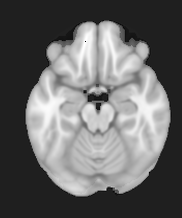
\includegraphics[height=0.5cm]{data/mris/slice_0.png}
					};
					\node[] at \patientlocation{(0, -0.5*\mrivsep)} {
						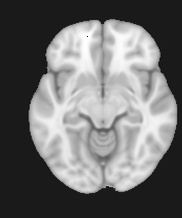
\includegraphics[height=0.5cm]{data/mris/slice_1.png}
					};
					\node[] at \patientlocation{(1 * \mrihsep, -0.5*\mrivsep)} {
						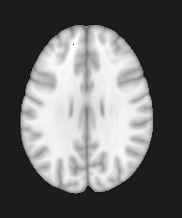
\includegraphics[height=0.5cm]{data/mris/slice_2.png}
					};
					\node[] at \patientlocation{(-1 * \mrihsep, 0.5*\mrivsep)} {
						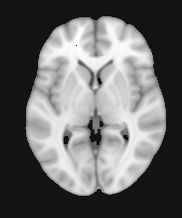
\includegraphics[height=0.5cm]{data/mris/slice_3.png}
					};
					\node[] at \patientlocation{(0, 0.5*\mrivsep)} {
						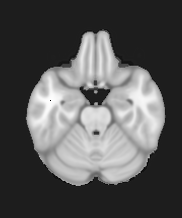
\includegraphics[height=0.5cm]{data/mris/slice_4.png}
					};
					\node[] at \patientlocation{(1 * \mrihsep, 0.5*\mrivsep)} {
						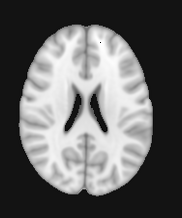
\includegraphics[height=0.5cm]{data/mris/slice_5.png}
					};

					\node[] at \controllocation{(-1 * \mrihsep, -0.5*\mrivsep)} {
						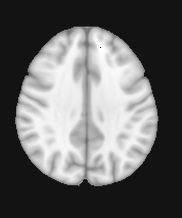
\includegraphics[height=0.5cm]{data/mris/slice_6.png}
					};
					\node[] at \controllocation{(0, -0.5*\mrivsep)} {
						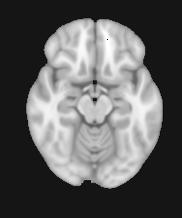
\includegraphics[height=0.5cm]{data/mris/slice_7.png}
					};
					\node[] at \controllocation{(1 * \mrihsep, -0.5*\mrivsep)} {
						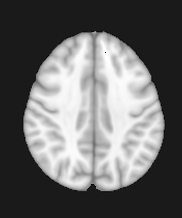
\includegraphics[height=0.5cm]{data/mris/slice_8.png}
					};
					\node[] at \controllocation{(-1 * \mrihsep, 0.5*\mrivsep)} {
						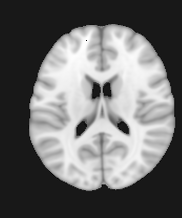
\includegraphics[height=0.5cm]{data/mris/slice_9.png}
					};
					\node[] at \controllocation{(0, 0.5*\mrivsep)} {
						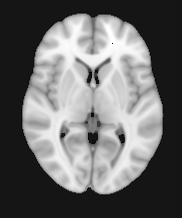
\includegraphics[height=0.5cm]{data/mris/slice_10.png}
					};
					\node[] at \controllocation{(1 * \mrihsep, 0.5*\mrivsep)} {
						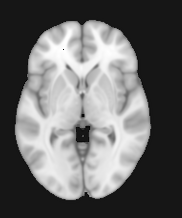
\includegraphics[height=0.5cm]{data/mris/slice_11.png}
					};
					\node[circle, inner sep=0pt, fill=none, outer sep=0pt, line width=0pt, draw=none] (n00) at \modellocation{(-3 * \hsep, 0)} {};

					\node[circle, minimum size=\nodesize, inner sep=0pt, fill=train-fill!35, outer sep=0pt, line width=0pt, draw=train-fill!35] (n10) at \modellocation{(-2 * \hsep, 2 * \vsep)} {};
					\node[circle, minimum size=\nodesize, inner sep=0pt, fill=train-fill, outer sep=0pt, line width=0pt, draw=train-fill] (n11) at \modellocation{(-2 * \hsep, 1 * \vsep)} {};
					\node[circle, minimum size=\nodesize, inner sep=0pt, fill=train-fill!15, outer sep=0pt, line width=0pt, draw=train-fill!15] (n12) at \modellocation{(-2 * \hsep, 0)} {};
					\node[circle, minimum size=\nodesize, inner sep=0pt, fill=train-fill!85, outer sep=0pt, line width=0pt, draw=train-fill!85] (n13) at \modellocation{(-2 * \hsep, -1 * \vsep)} {};
					\node[circle, minimum size=\nodesize, inner sep=0pt, fill=train-fill!90, outer sep=0pt, line width=0pt, draw=train-fill!90] (n14) at \modellocation{(-2 * \hsep, -2 * \vsep)} {};

					\node[circle, minimum size=\nodesize, inner sep=0pt, fill=train-fill!55, outer sep=0pt, line width=0pt, draw=train-fill!55] (n20) at \modellocation{(-1 * \hsep, 1.5 * \vsep)} {};
					\node[circle, minimum size=\nodesize, inner sep=0pt, fill=train-fill!20, outer sep=0pt, line width=0pt, draw=train-fill!20] (n21) at \modellocation{(-1 * \hsep, 0.5 * \vsep)} {};
					\node[circle, minimum size=\nodesize, inner sep=0pt, fill=train-fill!90, outer sep=0pt, line width=0pt, draw=train-fill!50] (n22) at \modellocation{(-1 * \hsep, -0.5 * \vsep)} {};
					\node[circle, minimum size=\nodesize, inner sep=0pt, fill=train-fill!35, outer sep=0pt, line width=0pt, draw=train-fill!35] (n23) at \modellocation{(-1 * \hsep, -1.5 * \vsep)} {};

					\node[circle, minimum size=\nodesize, inner sep=0pt, fill=train-fill!95, outer sep=0pt, line width=0pt, draw=train-fill!65] (n30) at \modellocation{(0 * \hsep, 1.5 * \vsep)} {};
					\node[circle, minimum size=\nodesize, inner sep=0pt, fill=train-fill!20, outer sep=0pt, line width=0pt, draw=train-fill!20] (n31) at \modellocation{(0 * \hsep, 0.5 * \vsep)} {};
					\node[circle, minimum size=\nodesize, inner sep=0pt, fill=train-fill!90, outer sep=0pt, line width=0pt, draw=train-fill!90] (n32) at \modellocation{(0 * \hsep, -0.5 * \vsep)} {};
					\node[circle, minimum size=\nodesize, inner sep=0pt, fill=train-fill!80, outer sep=0pt, line width=0pt, draw=train-fill!80] (n33) at \modellocation{(0 * \hsep, -1.5 * \vsep)} {};

					\node[circle, minimum size=\nodesize, inner sep=0pt, fill=train-fill!50, outer sep=0pt, line width=0pt, draw=train-fill!50] (n40) at \modellocation{(1 * \hsep, 1*\vsep)} {};
					\node[circle, minimum size=\nodesize, inner sep=0pt, fill=train-fill!90, outer sep=0pt, line width=0pt, draw=train-fill!70] (n41) at \modellocation{(1 * \hsep, 0*\vsep)} {};
					\node[circle, minimum size=\nodesize, inner sep=0pt, fill=train-fill!70, outer sep=0pt, line width=0pt, draw=train-fill!30] (n42) at \modellocation{(1 * \hsep, -1*\vsep)} {};

					\node[circle, minimum size=\nodesize, inner sep=0pt, fill=train-fill, outer sep=0pt, line width=0pt, draw=train-fill] (n50) at \modellocation{(2 * \hsep, 1*\vsep)} {};
					\node[circle, minimum size=\nodesize, inner sep=0pt, fill=train-fill!70, outer sep=0pt, line width=0pt, draw=train-fill!70] (n51) at \modellocation{(2 * \hsep, 0*\vsep)} {};
					\node[circle, minimum size=\nodesize, inner sep=0pt, fill=train-fill!30, outer sep=0pt, line width=0pt, draw=train-fill!30] (n52) at \modellocation{(2 * \hsep, -1*\vsep)} {};

					\node[circle, minimum size=\nodesize, inner sep=0pt, fill=train-fill!80, outer sep=0pt, line width=0pt, draw=train-fill!65] (n60) at \modellocation{(3 * \hsep, 0)} {};

					\node[] (loss) at (1+2*4.85, -2.2) {\scriptsize{$logloss(y, \hat{y})$}};

					\draw[
						color=train-fill!35,
						\innerarrow-\innerarrow,
						line width=\arrowwidth
					] (n00) to [out=20,in=200] (n10) {};
					\draw[
						color=train-fill,
						\innerarrow-\innerarrow,
						line width=\arrowwidth
					] (n00) to [out=10,in=190] (n11) {};
					\draw[
						color=train-fill!15,
						\innerarrow-\innerarrow,
						line width=\arrowwidth
					] (n00) to [out=0,in=180] (n12) {};
					\draw[
						color=train-fill!85,
						\innerarrow-\innerarrow,
						line width=\arrowwidth
					] (n00) to [out=-10,in=170] (n13) {};
					\draw[
						color=train-fill!90,
						\innerarrow-\innerarrow,
						line width=\arrowwidth
					] (n00) to [out=-20,in=160] (n14) {};

					\draw[
						color=train-fill!35,
						\innerarrow-\innerarrow,
						line width=\arrowwidth
					] (n10) to [out=-5,in=175] (n20) {};
					\draw[
						color=train-fill!10,
						\innerarrow-\innerarrow,
						line width=\arrowwidth
					] (n10) to [out=-15,in=165] (n21) {};
					\draw[
						color=train-fill!70,
						\innerarrow-\innerarrow,
						line width=\arrowwidth
					] (n10) to [out=-25,in=155] (n22) {};
					\draw[
						color=train-fill!50,
						\innerarrow-\innerarrow,
						line width=\arrowwidth
					] (n10) to [out=-35,in=145] (n23) {};

					\draw[
						color=train-fill!30,
						\innerarrow-\innerarrow,
						line width=\arrowwidth
					] (n11) to [out=5,in=185] (n20) {};
					\draw[
						color=train-fill!25,
						\innerarrow-\innerarrow,
						line width=\arrowwidth
					] (n11) to [out=-5,in=175] (n21) {};
					\draw[
						color=train-fill!95,
						\innerarrow-\innerarrow,
						line width=\arrowwidth
					] (n11) to [out=-15,in=165] (n22) {};
					\draw[
						color=train-fill!35,
						\innerarrow-\innerarrow,
						line width=\arrowwidth
					] (n11) to [out=-25,in=155] (n23) {};

					\draw[
						color=train-fill!70,
						\innerarrow-\innerarrow,
						line width=\arrowwidth
					] (n12) to [out=15,in=195] (n20) {};
					\draw[
						color=train-fill!20,
						\innerarrow-\innerarrow,
						line width=\arrowwidth
					] (n12) to [out=5,in=185] (n21) {};
					\draw[
						color=train-fill!80,
						\innerarrow-\innerarrow,
						line width=\arrowwidth
					] (n12) to [out=-5,in=175] (n22) {};
					\draw[
						color=train-fill,
						\innerarrow-\innerarrow,
						line width=\arrowwidth
					] (n12) to [out=-15,in=165] (n23) {};

					\draw[
						color=train-fill!40,
						\innerarrow-\innerarrow,
						line width=\arrowwidth
					] (n13) to [out=25,in=205] (n20) {};
					\draw[
						color=train-fill!35,
						\innerarrow-\innerarrow,
						line width=\arrowwidth
					] (n13) to [out=15,in=195] (n21) {};
					\draw[
						color=train-fill!20,
						\innerarrow-\innerarrow,
						line width=\arrowwidth
					] (n13) to [out=5,in=185] (n22) {};
					\draw[
						color=white,
						\innerarrow-\innerarrow,
						line width=\arrowwidth
					] (n13) to [out=-5,in=175] (n23) {};

					\draw[
						color=train-fill!40,
						\innerarrow-\innerarrow,
						line width=\arrowwidth
					] (n14) to [out=35,in=215] (n20) {};
					\draw[
						color=train-fill!85,
						\innerarrow-\innerarrow,
						line width=\arrowwidth
					] (n14) to [out=25,in=205] (n21) {};
					\draw[
						color=train-fill!35,
						\innerarrow-\innerarrow,
						line width=\arrowwidth
					] (n14) to [out=15,in=195] (n22) {};
					\draw[
						color=train-fill,
						\innerarrow-\innerarrow,
						line width=\arrowwidth
					] (n14) to [out=5,in=185] (n23) {};

					\draw[
						color=train-fill!85,
						\innerarrow-\innerarrow,
						line width=\arrowwidth
					] (n20) to [out=0,in=180] (n30) {};
					\draw[
						color=train-fill!50,
						\innerarrow-\innerarrow,
						line width=\arrowwidth
					] (n20) to [out=-10,in=170] (n31) {};
					\draw[
						color=train-fill!75,
						\innerarrow-\innerarrow,
						line width=\arrowwidth
					] (n20) to [out=-20,in=160] (n32) {};
					\draw[
						color=white,
						\innerarrow-\innerarrow,
						line width=\arrowwidth
					] (n20) to [out=-30,in=150] (n33) {};

					\draw[
						color=train-fill,
						\innerarrow-\innerarrow,
						line width=\arrowwidth
					] (n21) to [out=10,in=190] (n30) {};
					\draw[
						color=train-fill!30,
						\innerarrow-\innerarrow,
						line width=\arrowwidth
					] (n21) to [out=0,in=180] (n31) {};
					\draw[
						color=train-fill!25,
						\innerarrow-\innerarrow,
						line width=\arrowwidth
					] (n21) to [out=-10,in=170] (n32) {};
					\draw[
						color=white,
						\innerarrow-\innerarrow,
						line width=\arrowwidth
					] (n21) to [out=-20,in=160] (n33) {};

					\draw[
						color=train-fill!35,
						\innerarrow-\innerarrow,
						line width=\arrowwidth
					] (n22) to [out=20,in=200] (n30) {};
					\draw[
						color=train-fill!95,
						\innerarrow-\innerarrow,
						line width=\arrowwidth
					] (n22) to [out=10,in=190] (n31) {};
					\draw[
						color=train-fill!80,
						\innerarrow-\innerarrow,
						line width=\arrowwidth
					] (n22) to [out=0,in=180] (n32) {};
					\draw[
						color=white,
						\innerarrow-\innerarrow,
						line width=\arrowwidth
					] (n22) to [out=-10,in=170] (n33) {};

					\draw[
						color=train-fill!45,
						\innerarrow-\innerarrow,
						line width=\arrowwidth
					] (n23) to [out=30,in=210] (n30) {};
					\draw[
						color=train-fill!70,
						\innerarrow-\innerarrow,
						line width=\arrowwidth
					] (n23) to [out=20,in=200] (n31) {};
					\draw[
						color=train-fill!10,
						\innerarrow-\innerarrow,
						line width=\arrowwidth
					] (n23) to [out=10,in=190] (n32) {};
					\draw[
						color=train-fill!20,
						\innerarrow-\innerarrow,
						line width=\arrowwidth
					] (n23) to [out=0,in=180] (n33) {};

					\draw[
						color=train-fill!50,
						\innerarrow-\innerarrow,
						line width=\arrowwidth
					] (n30) to [out=-5,in=175] (n40) {};
					\draw[
						color=train-fill!30,
						\innerarrow-\innerarrow,
						line width=\arrowwidth
					] (n30) to [out=-15,in=165] (n41) {};
					\draw[
						color=train-fill,
						\innerarrow-\innerarrow,
						line width=\arrowwidth
					] (n30) to [out=-25,in=155] (n42) {};

					\draw[
						color=train-fill!45,
						\innerarrow-\innerarrow,
						line width=\arrowwidth
					] (n31) to [out=5,in=185] (n40) {};
					\draw[
						color=train-fill!90,
						\innerarrow-\innerarrow,
						line width=\arrowwidth
					] (n31) to [out=-5,in=175] (n41) {};
					\draw[
						color=train-fill!45,
						\innerarrow-\innerarrow,
						line width=\arrowwidth
					] (n31) to [out=-15,in=165] (n42) {};

					\draw[
						color=train-fill!15,
						\innerarrow-\innerarrow,
						line width=\arrowwidth
					] (n32) to [out=15,in=195] (n40) {};
					\draw[
						color=train-fill!70,
						\innerarrow-\innerarrow,
						line width=\arrowwidth
					] (n32) to [out=5,in=185] (n41) {};
					\draw[
						color=train-fill!50,
						\innerarrow-\innerarrow,
						line width=\arrowwidth
					] (n32) to [out=-5,in=175] (n42) {};

					\draw[
						color=train-fill!40,
						\innerarrow-\innerarrow,
						line width=\arrowwidth
					] (n33) to [out=25,in=205] (n40) {};
					\draw[
						color=train-fill!20,
						\innerarrow-\innerarrow,
						line width=\arrowwidth
					] (n33) to [out=15,in=195] (n41) {};
					\draw[
						color=train-fill!90,
						\innerarrow-\innerarrow,
						line width=\arrowwidth
					] (n33) to [out=5,in=185] (n42) {};

					\draw[
						color=train-fill!25,
						\innerarrow-\innerarrow,
						line width=\arrowwidth
					] (n40) to [out=0,in=180] (n50) {};
					\draw[
						color=train-fill!15,
						\innerarrow-\innerarrow,
						line width=\arrowwidth
					] (n40) to [out=-10,in=170] (n51) {};
					\draw[
						color=train-fill,
						\innerarrow-\innerarrow,
						line width=\arrowwidth
					] (n40) to [out=-20,in=160] (n52) {};

					\draw[
						color=train-fill!35,
						\innerarrow-\innerarrow,
						line width=\arrowwidth
					] (n41) to [out=10,in=190] (n50) {};
					\draw[
						color=train-fill!10,
						\innerarrow-\innerarrow,
						line width=\arrowwidth
					] (n41) to [out=0,in=180] (n51) {};
					\draw[
						color=train-fill!90,
						\innerarrow-\innerarrow,
						line width=\arrowwidth
					] (n41) to [out=-10,in=170] (n52) {};

					\draw[
						color=train-fill!50,
						\innerarrow-\innerarrow,
						line width=\arrowwidth
					] (n42) to [out=20,in=200] (n50) {};
					\draw[
						color=train-fill!40,
						\innerarrow-\innerarrow,
						line width=\arrowwidth
					] (n42) to [out=10,in=190] (n51) {};
					\draw[
						color=train-fill!20,
						\innerarrow-\innerarrow,
						line width=\arrowwidth
					] (n42) to [out=0,in=180] (n52) {};

					\draw[
						color=train-fill!80,
						\innerarrow-\innerarrow,
						line width=\arrowwidth,
					] (n50) to [out=-10,in=170] (n60) {};
					\draw[
						color=train-fill!90,
						\innerarrow-\innerarrow,
						line width=\arrowwidth,
					] (n51) to [out=0,in=180] (n60) {};
					\draw[
						color=train-fill!30,
						\innerarrow-\innerarrow,
						line width=\arrowwidth,
					] (n52) to [out=10,in=190] (n60) {};

					\draw[black] (n00.center) --
								($ (n00) + (0, 2*\vsep+0.5*\nodesize+2pt) $) --
								($ (n00) + (6*\hsep+0.5*\nodesize+2pt, 2*\vsep+0.5*\nodesize+2pt) $) --
								($ (n00) + (6*\hsep+0.5*\nodesize+2pt, -2*\vsep-0.5*\nodesize-2pt) $) --
								($ (n00) + (0, -2*\vsep-0.5*\nodesize-2pt) $) --
								(n00.center);

					\node[] at ($ (n30) + (0, \vsep+0.5*\nodesize) $) {\scriptsize{CNN}};

					\draw[
						color=outercolor,
						-\outerarrow,
						line width=0.1cm
					] \patientlocation{(0.65, 0)} to [out=0,in=180] (n00) {};
					\draw[
						color=outercolor,
						-\outerarrow,
						line width=0.1cm
					] \controllocation{(0.65, 0)} to [out=0,in=180] (n00) {};
					\draw[
						color=outercolor,
						\outerarrow-\outerarrow,
						line width=0.1cm
					] (n60) to [out=0,in=180] (loss) {};
				\end{tikzpicture}
			}
		}
		\newline
		\noindent
		\scalebox{0.4}{
			\hspace{3cm}
			\fbox{
				\begin{tikzpicture}
					\newcommand{\mrivsep}{0.52}
					\newcommand{\mrihsep}{0.44}

					\node[anchor=north west] at (0, 0.1) {\footnotesize{2. Apply model and LRP for individual-level predictions and relevance maps}};
					\node[anchor=north east] at (\plotwidth, 0) {};

					\newcommand{\mrilocation}[1]{($ (1, -2.2) + ####1 $)}
					\newcommand{\modellocation}[1]{($ (0.5 * \plotwidth, -2.2) + ####1 $)}
					\newcommand{\lrplocation}[1]{($ (0.5 * \plotwidth, -5.2) + ####1 $)}
					\def\maplocation{(1, -5.2)}

					\node[anchor=south, align=center, font=\scriptsize\linespread{0.85}\selectfont] at \mrilocation{(0, 0.92)} {All\\subjects};

					\newcommand{\mrialpha}{0.2}
					\colorlet{predict-fill}{cb-blue}
					\colorlet{lrp-fill}{red}

					\node[] at \mrilocation{(-1 * \mrihsep, -1.5*\mrivsep)} {
						{\transparent{\mrialpha}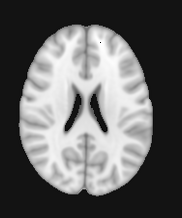
\includegraphics[height=0.5cm]{data/mris/slice_5.png}}
					};
					\node[] at \mrilocation{(0, -1.5*\mrivsep)} {
						{\transparent{\mrialpha}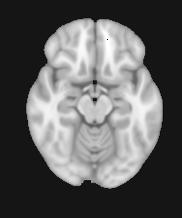
\includegraphics[height=0.5cm]{data/mris/slice_7.png}}
					};
					\node[] at \mrilocation{(1 * \mrihsep, -1.5*\mrivsep)} {
						{\transparent{\mrialpha}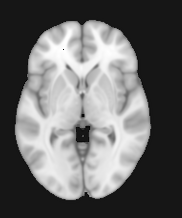
\includegraphics[height=0.5cm]{data/mris/slice_11.png}}
					};
					\node[] at \mrilocation{(-1 * \mrihsep, -0.5*\mrivsep)} {
						{\transparent{\mrialpha}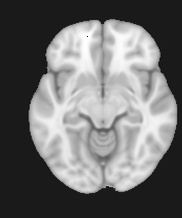
\includegraphics[height=0.5cm]{data/mris/slice_1.png}}
					};
					\node[] at \mrilocation{(0, -0.5*\mrivsep)} {
						{\transparent{\mrialpha}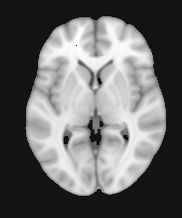
\includegraphics[height=0.5cm]{data/mris/slice_3.png}}
					};
					\node[inner sep=0pt, outer sep=0pt] (input) at \mrilocation{(1 * \mrihsep, -0.5*\mrivsep)} {
						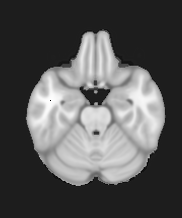
\includegraphics[height=0.5cm]{data/mris/slice_4.png}
					};
					\node[] at \mrilocation{(-1 * \mrihsep, 0.5*\mrivsep)} {
						{\transparent{\mrialpha}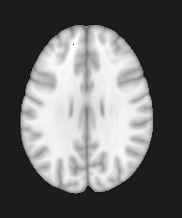
\includegraphics[height=0.5cm]{data/mris/slice_2.png}}
					};
					\node[] at \mrilocation{(0, 0.5*\mrivsep)} {
						{\transparent{\mrialpha}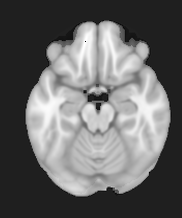
\includegraphics[height=0.5cm]{data/mris/slice_0.png}}
					};
					\node[] at \mrilocation{(1 * \mrihsep, 0.5*\mrivsep)} {
						{\transparent{\mrialpha}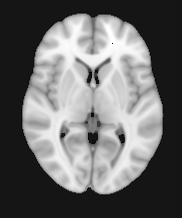
\includegraphics[height=0.5cm]{data/mris/slice_10.png}}
					};
					\node[] at \mrilocation{(-1 * \mrihsep, 1.5*\mrivsep)} {
						{\transparent{\mrialpha}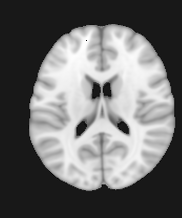
\includegraphics[height=0.5cm]{data/mris/slice_9.png}}
					};
					\node[] at \mrilocation{(0, 1.5*\mrivsep)} {
						{\transparent{\mrialpha}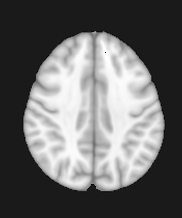
\includegraphics[height=0.5cm]{data/mris/slice_8.png}}
					};
					\node[] at \mrilocation{(1 * \mrihsep, 1.5*\mrivsep)} {
						{\transparent{\mrialpha}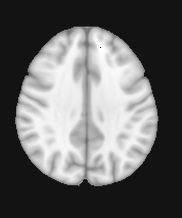
\includegraphics[height=0.5cm]{data/mris/slice_6.png}}
					};

					\node[circle, inner sep=0pt, fill=none, outer sep=0pt, line width=0pt, draw=none] (n00) at \modellocation{(-3 * \hsep, 0)} {};

					\node[circle, minimum size=\nodesize, inner sep=0pt, fill=predict-fill!85, outer sep=0pt, line width=0pt, draw=predict-fill!85] (n10) at \modellocation{(-2 * \hsep, 2 * \vsep)} {};
					\node[circle, minimum size=\nodesize, inner sep=0pt, fill=predict-fill, outer sep=0pt, line width=0pt, draw=predict-fill] (n11) at \modellocation{(-2 * \hsep, 1 * \vsep)} {};
					\node[circle, minimum size=\nodesize, inner sep=0pt, fill=predict-fill!75, outer sep=0pt, line width=0pt, draw=predict-fill!75] (n12) at \modellocation{(-2 * \hsep, 0)} {};
					\node[circle, minimum size=\nodesize, inner sep=0pt, fill=predict-fill!15, outer sep=0pt, line width=0pt, draw=predict-fill!15] (n13) at \modellocation{(-2 * \hsep, -1 * \vsep)} {};
					\node[circle, minimum size=\nodesize, inner sep=0pt, fill=predict-fill!50, outer sep=0pt, line width=0pt, draw=predict-fill!50] (n14) at \modellocation{(-2 * \hsep, -2 * \vsep)} {};

					\node[circle, minimum size=\nodesize, inner sep=0pt, fill=predict-fill!15, outer sep=0pt, line width=0pt, draw=predict-fill!15] (n20) at \modellocation{(-1 * \hsep, 1.5 * \vsep)} {};
					\node[circle, minimum size=\nodesize, inner sep=0pt, fill=predict-fill!65, outer sep=0pt, line width=0pt, draw=predict-fill!65] (n21) at \modellocation{(-1 * \hsep, 0.5 * \vsep)} {};
					\node[circle, minimum size=\nodesize, inner sep=0pt, fill=predict-fill!90, outer sep=0pt, line width=0pt, draw=predict-fill!90] (n22) at \modellocation{(-1 * \hsep, -0.5 * \vsep)} {};
					\node[circle, minimum size=\nodesize, inner sep=0pt, fill=predict-fill!40, outer sep=0pt, line width=0pt, draw=predict-fill!40] (n23) at \modellocation{(-1 * \hsep, -1.5 * \vsep)} {};

					\node[circle, minimum size=\nodesize, inner sep=0pt, fill=predict-fill!80, outer sep=0pt, line width=0pt, draw=predict-fill!80] (n30) at \modellocation{(0 * \hsep, 1.5 * \vsep)} {};
					\node[circle, minimum size=\nodesize, inner sep=0pt, fill=predict-fill!55, outer sep=0pt, line width=0pt, draw=predict-fill!55] (n31) at \modellocation{(0 * \hsep, 0.5 * \vsep)} {};
					\node[circle, minimum size=\nodesize, inner sep=0pt, fill=predict-fill!15, outer sep=0pt, line width=0pt, draw=predict-fill!15] (n32) at \modellocation{(0 * \hsep, -0.5 * \vsep)} {};
					\node[circle, minimum size=\nodesize, inner sep=0pt, fill=predict-fill!75, outer sep=0pt, line width=0pt, draw=predict-fill!75] (n33) at \modellocation{(0 * \hsep, -1.5 * \vsep)} {};

					\node[circle, minimum size=\nodesize, inner sep=0pt, fill=predict-fill, outer sep=0pt, line width=0pt, draw=predict-fill] (n40) at \modellocation{(1 * \hsep, 1*\vsep)} {};
					\node[circle, minimum size=\nodesize, inner sep=0pt, fill=predict-fill!20, outer sep=0pt, line width=0pt, draw=predict-fill!20] (n41) at \modellocation{(1 * \hsep, 0*\vsep)} {};
					\node[circle, minimum size=\nodesize, inner sep=0pt, fill=predict-fill!15, outer sep=0pt, line width=0pt, draw=predict-fill!15] (n42) at \modellocation{(1 * \hsep, -1*\vsep)} {};

					\node[circle, minimum size=\nodesize, inner sep=0pt, fill=predict-fill!75, outer sep=0pt, line width=0pt, draw=predict-fill!75] (n50) at \modellocation{(2 * \hsep, 1*\vsep)} {};
					\node[circle, minimum size=\nodesize, inner sep=0pt, fill=predict-fill!35, outer sep=0pt, line width=0pt, draw=predict-fill!35] (n51) at \modellocation{(2 * \hsep, 0*\vsep)} {};
					\node[circle, minimum size=\nodesize, inner sep=0pt, fill=predict-fill!65, outer sep=0pt, line width=0pt, draw=predict-fill!65] (n52) at \modellocation{(2 * \hsep, -1*\vsep)} {};

					\node[circle, minimum size=\nodesize, inner sep=0pt, fill=predict-fill!85, outer sep=0pt, line width=0pt, draw=predict-fill!85] (output) at \modellocation{(3 * \hsep, 0)} {};

					\node[] (diagnosis) at (1+2*4.85, -2.2) {\scriptsize{$\widehat{diagnosis}$}};

					\draw[
						color=predict-fill!85,
						-\innerarrow,
						line width=\arrowwidth
					] (n00) to [out=20,in=200] (n10) {};
					\draw[
						color=predict-fill,
						-\innerarrow,
						line width=\arrowwidth
					] (n00) to [out=10,in=190] (n11) {};
					\draw[
						color=predict-fill!75,
						-\innerarrow,
						line width=\arrowwidth
					] (n00) to [out=0,in=180] (n12) {};
					\draw[
						color=predict-fill!15,
						-\innerarrow,
						line width=\arrowwidth
					] (n00) to [out=-10,in=170] (n13) {};
					\draw[
						color=predict-fill!50,
						-\innerarrow,
						line width=\arrowwidth
					] (n00) to [out=-20,in=160] (n14) {};

					\draw[
						color=predict-fill!75,
						-\innerarrow,
						line width=\arrowwidth
					] (n10) to [out=-5,in=175] (n20) {};
					\draw[
						color=predict-fill!50,
						-\innerarrow,
						line width=\arrowwidth
					] (n10) to [out=-15,in=165] (n21) {};
					\draw[
						color=predict-fill!55,
						-\innerarrow,
						line width=\arrowwidth
					] (n10) to [out=-25,in=155] (n22) {};
					\draw[
						color=predict-fill!85,
						-\innerarrow,
						line width=\arrowwidth
					] (n10) to [out=-35,in=145] (n23) {};

					\draw[
						color=predict-fill!45,
						-\innerarrow,
						line width=\arrowwidth
					] (n11) to [out=5,in=185] (n20) {};
					\draw[
						color=predict-fill!50,
						-\innerarrow,
						line width=\arrowwidth
					] (n11) to [out=-5,in=175] (n21) {};
					\draw[
						color=predict-fill,
						-\innerarrow,
						line width=\arrowwidth
					] (n11) to [out=-15,in=165] (n22) {};
					\draw[
						color=predict-fill!15,
						-\innerarrow,
						line width=\arrowwidth
					] (n11) to [out=-25,in=155] (n23) {};

					\draw[
						color=predict-fill!35,
						-\innerarrow,
						line width=\arrowwidth
					] (n12) to [out=15,in=195] (n20) {};
					\draw[
						color=predict-fill!90,
						-\innerarrow,
						line width=\arrowwidth
					] (n12) to [out=5,in=185] (n21) {};
					\draw[
						color=predict-fill!80,
						-\innerarrow,
						line width=\arrowwidth
					] (n12) to [out=-5,in=175] (n22) {};
					\draw[
						color=predict-fill!20,
						-\innerarrow,
						line width=\arrowwidth
					] (n12) to [out=-15,in=165] (n23) {};

					\draw[
						color=predict-fill!55,
						-\innerarrow,
						line width=\arrowwidth
					] (n13) to [out=25,in=205] (n20) {};
					\draw[
						color=predict-fill!65,
						-\innerarrow,
						line width=\arrowwidth
					] (n13) to [out=15,in=195] (n21) {};
					\draw[
						color=predict-fill!35,
						-\innerarrow,
						line width=\arrowwidth
					] (n13) to [out=5,in=185] (n22) {};
					\draw[
						color=predict-fill!45,
						-\innerarrow,
						line width=\arrowwidth
					] (n13) to [out=-5,in=175] (n23) {};

					\draw[
						color=predict-fill!10,
						-\innerarrow,
						line width=\arrowwidth
					] (n14) to [out=35,in=215] (n20) {};
					\draw[
						color=predict-fill!90,
						-\innerarrow,
						line width=\arrowwidth
					] (n14) to [out=25,in=205] (n21) {};
					\draw[
						color=predict-fill!80,
						-\innerarrow,
						line width=\arrowwidth
					] (n14) to [out=15,in=195] (n22) {};
					\draw[
						color=predict-fill!35,
						-\innerarrow,
						line width=\arrowwidth
					] (n14) to [out=5,in=185] (n23) {};

					\draw[
						color=predict-fill!75,
						-\innerarrow,
						line width=\arrowwidth
					] (n20) to [out=0,in=180] (n30) {};
					\draw[
						color=predict-fill!50,
						-\innerarrow,
						line width=\arrowwidth
					] (n20) to [out=-10,in=170] (n31) {};
					\draw[
						color=predict-fill!85,
						-\innerarrow,
						line width=\arrowwidth
					] (n20) to [out=-20,in=160] (n32) {};
					\draw[
						color=predict-fill!45,
						-\innerarrow,
						line width=\arrowwidth
					] (n20) to [out=-30,in=150] (n33) {};

					\draw[
						color=predict-fill!20,
						-\innerarrow,
						line width=\arrowwidth
					] (n21) to [out=10,in=190] (n30) {};
					\draw[
						color=predict-fill!35,
						-\innerarrow,
						line width=\arrowwidth
					] (n21) to [out=0,in=180] (n31) {};
					\draw[
						color=predict-fill!15,
						-\innerarrow,
						line width=\arrowwidth
					] (n21) to [out=-10,in=170] (n32) {};
					\draw[
						color=predict-fill!90,
						-\innerarrow,
						line width=\arrowwidth
					] (n21) to [out=-20,in=160] (n33) {};

					\draw[
						color=predict-fill!65,
						-\innerarrow,
						line width=\arrowwidth
					] (n22) to [out=20,in=200] (n30) {};
					\draw[
						color=predict-fill!20,
						-\innerarrow,
						line width=\arrowwidth
					] (n22) to [out=10,in=190] (n31) {};
					\draw[
						color=predict-fill!30,
						-\innerarrow,
						line width=\arrowwidth
					] (n22) to [out=0,in=180] (n32) {};
					\draw[
						color=predict-fill!40,
						-\innerarrow,
						line width=\arrowwidth
					] (n22) to [out=-10,in=170] (n33) {};

					\draw[
						color=predict-fill,
						-\innerarrow,
						line width=\arrowwidth
					] (n23) to [out=30,in=210] (n30) {};
					\draw[
						color=predict-fill!15,
						-\innerarrow,
						line width=\arrowwidth
					] (n23) to [out=20,in=200] (n31) {};
					\draw[
						color=predict-fill!75,
						-\innerarrow,
						line width=\arrowwidth
					] (n23) to [out=10,in=190] (n32) {};
					\draw[
						color=predict-fill!35,
						-\innerarrow,
						line width=\arrowwidth
					] (n23) to [out=0,in=180] (n33) {};

					\draw[
						color=predict-fill!70,
						-\innerarrow,
						line width=\arrowwidth
					] (n30) to [out=-5,in=175] (n40) {};
					\draw[
						color=predict-fill!80,
						-\innerarrow,
						line width=\arrowwidth
					] (n30) to [out=-15,in=165] (n41) {};
					\draw[
						color=predict-fill!20,
						-\innerarrow,
						line width=\arrowwidth
					] (n30) to [out=-25,in=155] (n42) {};

					\draw[
						color=predict-fill!60,
						-\innerarrow,
						line width=\arrowwidth
					] (n31) to [out=5,in=185] (n40) {};
					\draw[
						color=predict-fill!95,
						-\innerarrow,
						line width=\arrowwidth
					] (n31) to [out=-5,in=175] (n41) {};
					\draw[
						color=predict-fill!35,
						-\innerarrow,
						line width=\arrowwidth
					] (n31) to [out=-15,in=165] (n42) {};

					\draw[
						color=predict-fill!75,
						-\innerarrow,
						line width=\arrowwidth
					] (n32) to [out=15,in=195] (n40) {};
					\draw[
						color=predict-fill!20,
						-\innerarrow,
						line width=\arrowwidth
					] (n32) to [out=5,in=185] (n41) {};
					\draw[
						color=predict-fill!15,
						-\innerarrow,
						line width=\arrowwidth
					] (n32) to [out=-5,in=175] (n42) {};

					\draw[
						color=predict-fill!40,
						-\innerarrow,
						line width=\arrowwidth
					] (n33) to [out=25,in=205] (n40) {};
					\draw[
						color=predict-fill!80,
						-\innerarrow,
						line width=\arrowwidth
					] (n33) to [out=15,in=195] (n41) {};
					\draw[
						color=predict-fill!50,
						-\innerarrow,
						line width=\arrowwidth
					] (n33) to [out=5,in=185] (n42) {};

					\draw[
						color=predict-fill!25,
						-\innerarrow,
						line width=\arrowwidth
					] (n40) to [out=0,in=180] (n50) {};
					\draw[
						color=predict-fill!50,
						-\innerarrow,
						line width=\arrowwidth
					] (n40) to [out=-10,in=170] (n51) {};
					\draw[
						color=predict-fill!45,
						-\innerarrow,
						line width=\arrowwidth
					] (n40) to [out=-20,in=160] (n52) {};

					\draw[
						color=predict-fill!90,
						-\innerarrow,
						line width=\arrowwidth
					] (n41) to [out=10,in=190] (n50) {};
					\draw[
						color=predict-fill!10,
						-\innerarrow,
						line width=\arrowwidth
					] (n41) to [out=0,in=180] (n51) {};
					\draw[
						color=predict-fill!75,
						-\innerarrow,
						line width=\arrowwidth
					] (n41) to [out=-10,in=170] (n52) {};

					\draw[
						color=predict-fill!60,
						-\innerarrow,
						line width=\arrowwidth
					] (n42) to [out=20,in=200] (n50) {};
					\draw[
						color=predict-fill!25,
						-\innerarrow,
						line width=\arrowwidth
					] (n42) to [out=10,in=190] (n51) {};
					\draw[
						color=predict-fill!15,
						-\innerarrow,
						line width=\arrowwidth
					] (n42) to [out=0,in=180] (n52) {};

					\draw[
						color=predict-fill!95,
						-\innerarrow,
						line width=\arrowwidth
					] (n50) to [out=-10,in=170] (output) {};
					\draw[
						color=predict-fill!25,
						-\innerarrow,
						line width=\arrowwidth
					] (n51) to [out=0,in=180] (output) {};
					\draw[
						color=predict-fill!50,
						-\innerarrow,
						line width=\arrowwidth
					] (n52) to [out=10,in=190] (output) {};

					\draw[black] (n00.center) --
								($ (n00) + (0, 2*\vsep+0.5*\nodesize+2pt) $) --
								($ (n00) + (6*\hsep+0.5*\nodesize+2pt, 2*\vsep+0.5*\nodesize+2pt) $) --
								($ (n00) + (6*\hsep+0.5*\nodesize+2pt, -2*\vsep-0.5*\nodesize-2pt) $) --
								($ (n00) + (0, -2*\vsep-0.5*\nodesize-2pt) $) -- (n00.center);

					\node[] at ($ (n30) + (0, \vsep+0.5*\nodesize) $) {\footnotesize{CNN}};

					\draw[
						color=outercolor,
						-\outerarrow,
						line width=0.1cm
					] (input) to [out=0,in=180] (n00) {};
					\draw[
						color=outercolor,
						-\outerarrow,
						line width=0.1cm
					] (output) to [out=0,in=180] (diagnosis) {};

					\node[circle, inner sep=0pt, fill=none, outer sep=0pt, line width=0pt, draw=none] (n00) at \lrplocation{(-3 * \hsep, 0)} {};

					\node[circle, minimum size=\nodesize, inner sep=0pt, fill={rgb:black,5;orange,1}, outer sep=0pt, line width=0pt, draw={rgb:black,5;orange,1}] (n10) at \lrplocation{(-2 * \hsep, 2 * \vsep)} {};
					\node[circle, minimum size=\nodesize, inner sep=0pt, fill={rgb:black,3;red,1}, outer sep=0pt, line width=0pt, draw={rgb:black,3;red,1}] (n11) at \lrplocation{(-2 * \hsep, 1 * \vsep)} {};
					\node[circle, minimum size=\nodesize, inner sep=0pt, fill=yellow, outer sep=0pt, line width=0pt, draw=yellow] (n12) at \lrplocation{(-2 * \hsep, 0)} {};
					\node[circle, minimum size=\nodesize, inner sep=0pt, fill=black, outer sep=0pt, line width=0pt, draw=black] (n13) at \lrplocation{(-2 * \hsep, -1 * \vsep)} {};
					\node[circle, minimum size=\nodesize, inner sep=0pt, fill=red, outer sep=0pt, line width=0pt, draw=red] (n14) at \lrplocation{(-2 * \hsep, -2 * \vsep)} {};

					\node[circle, minimum size=\nodesize, inner sep=0pt, fill={rgb:black,5;white,2;orange,1}, outer sep=0pt, line width=0pt, draw={rgb:black,5;white,2;orange,1}] (n20) at \lrplocation{(-1 * \hsep, 1.5 * \vsep)} {};
					\node[circle, minimum size=\nodesize, inner sep=0pt, fill={rgb:red,10;yellow,6}, outer sep=0pt, line width=0pt, draw={rgb:red,10;yellow,4}] (n21) at \lrplocation{(-1 * \hsep, 0.5 * \vsep)} {};
					\node[circle, minimum size=\nodesize, inner sep=0pt, fill={rgb:red,10;yellow,1}, outer sep=0pt, line width=0pt, draw={rgb:red,10;yellow,1}] (n22) at \lrplocation{(-1 * \hsep, -0.5 * \vsep)} {};
					\node[circle, minimum size=\nodesize, inner sep=0pt, fill={rgb:black,10;red,2}, outer sep=0pt, line width=0pt, draw={rgb:black,10;red,2}] (n23) at \lrplocation{(-1 * \hsep, -1.5 * \vsep)} {};

					\node[circle, minimum size=\nodesize, inner sep=0pt, fill={rgb:red,3;orange,2}, outer sep=0pt, line width=0pt, draw={rgb:red,3;orange,1}] (n30) at \lrplocation{(0 * \hsep, 1.5 * \vsep)} {};
					\node[circle, minimum size=\nodesize, inner sep=0pt, fill={rgb:yellow,3;orange,1}, outer sep=0pt, line width=0pt, draw={rgb:yellow,3;orange,1}] (n31) at \lrplocation{(0 * \hsep, 0.5 * \vsep)} {};
					\node[circle, minimum size=\nodesize, inner sep=0pt, fill={rgb:black,10;white,5;red,1}, outer sep=0pt, line width=0pt, draw={rgb:black,10;white,5;red,1}] (n32) at \lrplocation{(0 * \hsep, -0.5 * \vsep)} {};
					\node[circle, minimum size=\nodesize, inner sep=0pt, fill={rgb:gray,5;red,1}, outer sep=0pt, line width=0pt, draw={rgb:gray,5;red,1}] (n33) at \lrplocation{(0 * \hsep, -1.5 * \vsep)} {};

					\node[circle, minimum size=\nodesize, inner sep=0pt, fill={rgb:yellow,10;orange,1}, outer sep=0pt, line width=0pt, draw={rgb:yellow,10;orange,1}] (n40) at \lrplocation{(1 * \hsep, 1*\vsep)} {};
					\node[circle, minimum size=\nodesize, inner sep=0pt, fill={rgb:red,1}, outer sep=0pt, line width=0pt, draw={rgb:red,1}] (n41) at \lrplocation{(1 * \hsep, 0*\vsep)} {};
					\node[circle, minimum size=\nodesize, inner sep=0pt, fill={rgb:black,10;white,15;red,2}, outer sep=0pt, line width=0pt, draw={rgb:black,10;white,15;red,2}] (n42) at \lrplocation{(1 * \hsep, -1*\vsep)} {};

					\node[circle, minimum size=\nodesize, inner sep=0pt, fill={rgb:red,5;black,1;yellow,2}, outer sep=0pt, line width=0pt, draw={rgb:red,5;black,1;yellow,2}] (n50) at \lrplocation{(2 * \hsep, 1*\vsep)} {};
					\node[circle, minimum size=\nodesize, inner sep=0pt, fill={rgb:gray,5;red,1}, outer sep=0pt, line width=0pt, draw={rgb:gray,5;red,1}] (n51) at \lrplocation{(2 * \hsep, 0*\vsep)} {};
					\node[circle, minimum size=\nodesize, inner sep=0pt, fill={rgb:yellow,5;orange,1}, outer sep=0pt, line width=0pt, draw={rgb:yellow,5;orange,1}] (n52) at \lrplocation{(2 * \hsep, -1*\vsep)} {};

					\node[circle, minimum size=\nodesize, inner sep=0pt, fill={rgb:orange,7;yellow,4;black,1}, outer sep=0pt, line width=0pt, draw={rgb:orange,7;yellow,4;black,1}] (n60) at \lrplocation{(3 * \hsep, 0)} {};

					\draw[
						color={rgb:black,5;orange,1},
						\innerarrow-,
						line width=\arrowwidth
					] (n00) to [out=20,in=200] (n10) {};
					\draw[
						color={rgb:black,3;red,1},
						\innerarrow-,
						line width=\arrowwidth
					] (n00) to [out=10,in=190] (n11) {};
					\draw[
						color=yellow,
						\innerarrow-,
						line width=\arrowwidth
					] (n00) to [out=0,in=180] (n12) {};
					\draw[
						color=black,
						\innerarrow-,
						line width=\arrowwidth
					] (n00) to [out=-10,in=170] (n13) {};
					\draw[
						color=red,
						\innerarrow-,
						line width=\arrowwidth
					] (n00) to [out=-20,in=160] (n14) {};

					\draw[
						color={rgb:black,5;white,1;orange,1},
						\innerarrow-,
						line width=\arrowwidth
					] (n10) to [out=-5,in=175] (n20) {};
					\draw[
						color={rgb:black,3;orange,1},
						\innerarrow-,
						line width=\arrowwidth
					] (n10) to [out=-15,in=165] (n21) {};
					\draw[
						color={rgb:black,4;red,2;yellow,1},
						\innerarrow-,
						line width=\arrowwidth
					] (n10) to [out=-25,in=155] (n22) {};
					\draw[
						color={rgb:black,3;red,1},
						\innerarrow-,
						line width=\arrowwidth
					] (n10) to [out=-35,in=145] (n23) {};

					\draw[
						color={rgb:black,10;orange,2},
						\innerarrow-,
						line width=\arrowwidth
					] (n11) to [out=5,in=185] (n20) {};
					\draw[
						color={rgb:black,3;orange,1},
						\innerarrow-,
						line width=\arrowwidth
					] (n11) to [out=-5,in=175] (n21) {};
					\draw[
						color={rgb:black,3;red,1},
						\innerarrow-,
						line width=\arrowwidth
					] (n11) to [out=-15,in=165] (n22) {};
					\draw[
						color={rgb:black,10;red,1},
						\innerarrow-,
						line width=\arrowwidth
					] (n11) to [out=-25,in=155] (n23) {};

					\draw[
						color={rgb:black,5;orange,3},
						\innerarrow-,
						line width=\arrowwidth
					] (n12) to [out=15,in=195] (n20) {};
					\draw[
						color={rgb:red,3;yellow,5},
						\innerarrow-,
						line width=\arrowwidth
					] (n12) to [out=5,in=185] (n21) {};
					\draw[
						color={rgb:red,5;yellow,3},
						\innerarrow-,
						line width=\arrowwidth
					] (n12) to [out=-5,in=175] (n22) {};
					\draw[
						color={rgb:black,5;orange,2},
						\innerarrow-,
						line width=\arrowwidth
					] (n12) to [out=-15,in=165] (n23) {};

					\draw[
						color={rgb:black,5;red,1},
						\innerarrow-,
						line width=\arrowwidth
					] (n13) to [out=25,in=205] (n20) {};
					\draw[
						color={rgb:black,5;orange,2},
						\innerarrow-,
						line width=\arrowwidth
					] (n13) to [out=15,in=195] (n21) {};
					\draw[
						color={rgb:black,5;red,3},
						\innerarrow-,
						line width=\arrowwidth
					] (n13) to [out=5,in=185] (n22) {};
					\draw[
						color=black,
						\innerarrow-,
						line width=\arrowwidth
					] (n13) to [out=-5,in=175] (n23) {};

					\draw[
						color={rgb:black,5;orange,2},
						\innerarrow-,
						line width=\arrowwidth
					] (n14) to [out=35,in=215] (n20) {};
					\draw[
						color={rgb:red,3;orange,1},
						\innerarrow-,
						line width=\arrowwidth
					] (n14) to [out=25,in=205] (n21) {};
					\draw[
						color={rgb:red,5;yellow,2},
						\innerarrow-,
						line width=\arrowwidth
					] (n14) to [out=15,in=195] (n22) {};
					\draw[
						color={rgb:black,5;red,3},
						\innerarrow-,
						line width=\arrowwidth
					] (n14) to [out=5,in=185] (n23) {};

					\draw[
						color={rgb:black,1;red,1},
						\innerarrow-,
						line width=\arrowwidth
					] (n20) to [out=0,in=180] (n30) {};
					\draw[
						color={rgb:black,3;orange,1},
						\innerarrow-,
						line width=\arrowwidth
					] (n20) to [out=-10,in=170] (n31) {};
					\draw[
						color={rgb:black,10;red,1},
						\innerarrow-,
						line width=\arrowwidth
					] (n20) to [out=-20,in=160] (n32) {};
					\draw[
						color={rgb:black,5;red,1},
						\innerarrow-,
						line width=\arrowwidth
					] (n20) to [out=-30,in=150] (n33) {};

					\draw[
						color={rgb:orange,5;red,2},
						\innerarrow-,
						line width=\arrowwidth
					] (n21) to [out=10,in=190] (n30) {};
					\draw[
						color={rgb:yellow,10;orange,4},
						\innerarrow-,
						line width=\arrowwidth
					] (n21) to [out=0,in=180] (n31) {};
					\draw[
						color={rgb:black,2;red,1},
						\innerarrow-,
						line width=\arrowwidth
					] (n21) to [out=-10,in=170] (n32) {};
					\draw[
						color={rgb:black,1;orange,2;red,1},
						\innerarrow-,
						line width=\arrowwidth
					] (n21) to [out=-20,in=160] (n33) {};

					\draw[
						color={rgb:red,2;orange,1},
						\innerarrow-,
						line width=\arrowwidth
					] (n22) to [out=20,in=200] (n30) {};
					\draw[
						color={rgb:yellow,2;orange,1},
						\innerarrow-,
						line width=\arrowwidth
					] (n22) to [out=10,in=190] (n31) {};
					\draw[
						color={rgb:black,2;red,2},
						\innerarrow-,
						line width=\arrowwidth
					] (n22) to [out=0,in=180] (n32) {};
					\draw[
						color={rgb:black,2;orange,1},
						\innerarrow-,
						line width=\arrowwidth
					] (n22) to [out=-10,in=170] (n33) {};

					\draw[
						color={rgb:black,4;red,2},
						\innerarrow-,
						line width=\arrowwidth
					] (n23) to [out=30,in=210] (n30) {};
					\draw[
						color={rgb:orange,2;black,1},
						\innerarrow-,
						line width=\arrowwidth
					] (n23) to [out=20,in=200] (n31) {};
					\draw[
						color={rgb:black,5;orange,1},
						\innerarrow-,
						line width=\arrowwidth
					] (n23) to [out=10,in=190] (n32) {};
					\draw[
						color={rgb:black,5;red,2},
						\innerarrow-,
						line width=\arrowwidth
					] (n23) to [out=0,in=180] (n33) {};

					\draw[
						color={rgb:orange,3;red,1},
						\innerarrow-,
						line width=\arrowwidth
					] (n30) to [out=-5,in=175] (n40) {};
					\draw[
						color={rgb:gray,1;orange,1;red,2},
						\innerarrow-,
						line width=\arrowwidth
					] (n30) to [out=-15,in=165] (n41) {};
					\draw[
						color={rgb:orange,2;black,2;white,1},
						\innerarrow-,
						line width=\arrowwidth
					] (n30) to [out=-25,in=155] (n42) {};

					\draw[
						color={rgb:yellow,5;orange,1},
						\innerarrow-,
						line width=\arrowwidth
					] (n31) to [out=5,in=185] (n40) {};
					\draw[
						color={rgb:red,3;orange,1},
						\innerarrow-,
						line width=\arrowwidth
					] (n31) to [out=-5,in=175] (n41) {};
					\draw[
						color={rgb:gray,1;red,2},
						\innerarrow-,
						line width=\arrowwidth
					] (n31) to [out=-15,in=165] (n42) {};

					\draw[
						color={rgb:gray,3;orange,1},
						\innerarrow-,
						line width=\arrowwidth
					] (n32) to [out=15,in=195] (n40) {};
					\draw[
						color={rgb:gray,1;red,1},
						\innerarrow-,
						line width=\arrowwidth
					] (n32) to [out=5,in=185] (n41) {};
					\draw[
						color={rgb:gray,1},
						\innerarrow-,
						line width=\arrowwidth
					] (n32) to [out=-5,in=175] (n42) {};

					\draw[
						color={rgb:gray,2;orange,3},
						\innerarrow-,
						line width=\arrowwidth
					] (n33) to [out=25,in=205] (n40) {};
					\draw[
						color={rgb:gray,1;orange,1},
						\innerarrow-,
						line width=\arrowwidth
					] (n33) to [out=15,in=195] (n41) {};
					\draw[
						color={rgb:gray,3;red,1},
						\innerarrow-,
						line width=\arrowwidth
					] (n33) to [out=5,in=185] (n42) {};

					\draw[
						color={rgb:red,3;yellow,1},
						\innerarrow-,
						line width=\arrowwidth
					] (n40) to [out=0,in=180] (n50) {};
					\draw[
						color={rgb:gray,2;orange,1},
						\innerarrow-,
						line width=\arrowwidth
					] (n40) to [out=-10,in=170] (n51) {};
					\draw[
						color={rgb:yellow,10;orange,1},
						\innerarrow-,
						line width=\arrowwidth
					] (n40) to [out=-20,in=160] (n52) {};

					\draw[
						color={rgb:red,5;black,1;yellow,2},
						\innerarrow-,
						line width=\arrowwidth
					] (n41) to [out=10,in=190] (n50) {};
					\draw[
						color={rgb:gray,7;orange,3},
						\innerarrow-,
						line width=\arrowwidth
					] (n41) to [out=0,in=180] (n51) {};
					\draw[
						color={rgb:yellow,1;orange,2},
						\innerarrow-,
						line width=\arrowwidth
					] (n41) to [out=-10,in=170] (n52) {};

					\draw[
						color={rgb:gray,7;orange,2},
						\innerarrow-,
						line width=\arrowwidth
					] (n42) to [out=20,in=200] (n50) {};
					\draw[
						color={rgb:gray,5;red,1},
						\innerarrow-,
						line width=\arrowwidth
					] (n42) to [out=10,in=190] (n51) {};
					\draw[
						color={rgb:gray,5;red,1;black,2},
						\innerarrow-,
						line width=\arrowwidth
					] (n42) to [out=0,in=180] (n52) {};

					\draw[
						color={rgb:red,5;black,1;yellow,2},
						\innerarrow-,
						line width=\arrowwidth
					] (n50) to [out=-10,in=170] (n60) {};
					\draw[
						color={rgb:gray,5;red,1},
						\innerarrow-,
						line width=\arrowwidth
					] (n51) to [out=0,in=180] (n60) {};
					\draw[
						color={rgb:yellow,5;orange,1},
						\innerarrow-,
						line width=\arrowwidth
					] (n52) to [out=10,in=190] (n60) {};

					\draw[black] (n00.center) --
								($ (n00) + (0, 2*\vsep+0.5*\nodesize+2pt) $) --
								($ (n00) + (6*\hsep+0.5*\nodesize+2pt, 2*\vsep+0.5*\nodesize+2pt) $) --
								($ (n00) + (6*\hsep+0.5*\nodesize+2pt, -2*\vsep-0.5*\nodesize-2pt) $) --
								($ (n00) + (0, -2*\vsep-0.5*\nodesize-2pt) $) -- (n00.center);

					\node[] at ($ (n33) + (0, -1 * \vsep-0.5*\nodesize) $) {\scriptsize{LRP}};

					\draw[double distance=4pt, {Stealth[width=10pt,length=5pt]}-{Stealth[width=10pt,length=5pt]}, line width=1pt] \lrplocation{(0, 2*\vsep+0.5*\nodesize+2pt)} -- \modellocation{(0, -2*\vsep-0.5*\nodesize-2pt)};


					\draw[
						color=outercolor,
						-\outerarrow,
						line width=0.1cm
					] (output) to [out=270,in=90] (n60) {};

					\node[inner sep=0pt, outer sep=0pt] (map) at \maplocation {
						
\includegraphics[width=1cm]{data/averages/dementia.png}
					};

					\node[inner sep=0pt, outer sep=0pt,label={[align=center,font=\scriptsize\linespread{0.85}\selectfont]below:\textit{Relevance}\\ \textit{map}}] (map) at \maplocation {
						
\includegraphics[
							width=1cm,
							clip=true,
							trim = 128mm 232mm 64mm 0mm
						]{data/averages/dementia.png}
					};

					\draw[
						color=outercolor,
						-\outerarrow,
						line width=0.1cm
					] (n00) to [out=180,in=0] (map) {};
				\end{tikzpicture}
			}
		}
		\newline
		\noindent
		\scalebox{0.4}{
			\hspace{3cm}
			\fbox{
				\begin{tikzpicture}
					\newcommand{\mrivsep}{0.75}
					\newcommand{\mrihsep}{0.6}
					\newcommand{\mriwidth}{0.55cm}
					\newcommand{\mriheight}{0.7cm}

					\node[anchor=north west] at (0, 0.25) {\footnotesize{3. Validate relevance maps for diagnosed patients against the literature}};
					\node[anchor=north east] at (\plotwidth, 0) {};

					\newcommand{\patientlocation}[1]{($ (0.5 * \plotwidth - 4, -1.7) + ####1 $)}
					\newcommand{\comparisonlocation}[1]{($ (0.5 * \plotwidth, -1.7) + ####1 $)}
					\newcommand{\resultslocation}[1]{($ (0.5 * \plotwidth + 4, -1.7) + ####1 $)}


					\node[align=center, font=\scriptsize\linespread{0.85}\selectfont] at \patientlocation{(0, 1)} {Dementia\\patients};

					\node[] at \patientlocation{(-1 * \mrihsep, -0.5*\mrivsep)} {
						
\includegraphics[
							width=\mriwidth,
							height=\mriheight,
							clip=true,
							trim = 0mm 154mm 192mm 78mm
						]{data/averages/dementia.png}
					};
					\node[] at \patientlocation{(0, -0.5*\mrivsep)} {
						
\includegraphics[
							width=\mriwidth,
							height=\mriheight,
							clip=true,
							trim = 128mm 232mm 64mm 0mm
						]{data/averages/dementia.png}
					};
					\node[] at \patientlocation{(1 * \mrihsep, -0.5*\mrivsep)} {
						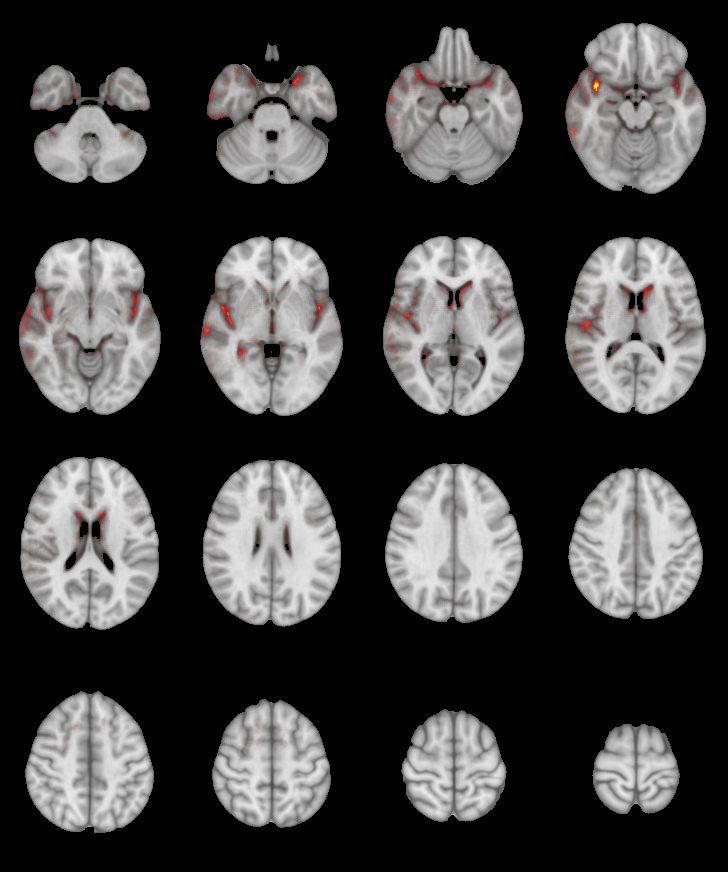
\includegraphics[
							width=\mriwidth,
							height=\mriheight,
							clip=true,
							trim = 64mm 154mm 128mm 78mm
						]{data/samples/subject2.png}
					};
					\node[] at \patientlocation{(-1 * \mrihsep, 0.5*\mrivsep)} {
						\scalebox{-1}[1]{
							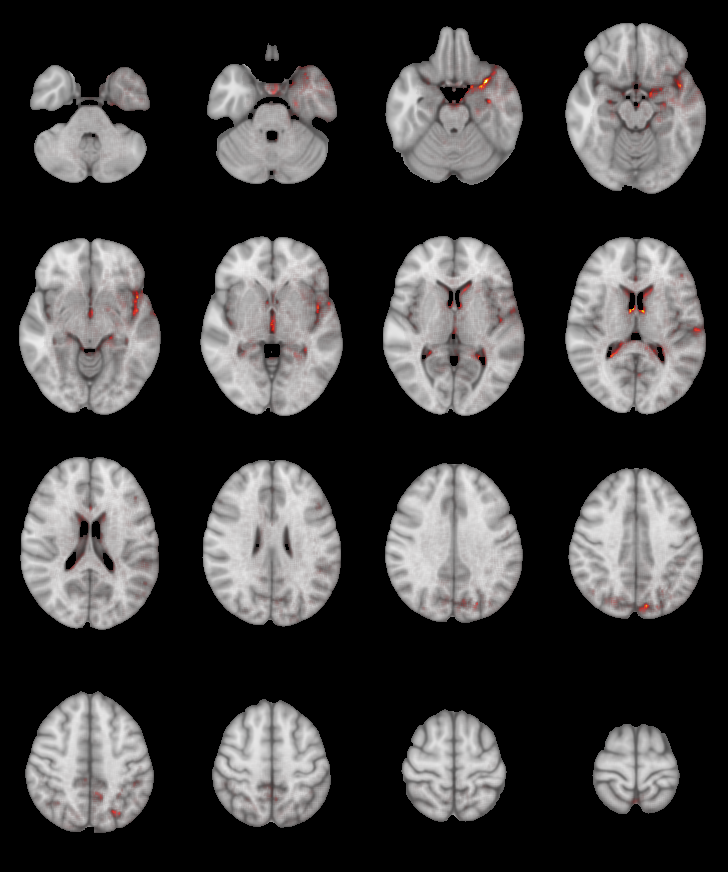
\includegraphics[
								width=\mriwidth,
								height=\mriheight,
								clip=true,
								trim = 128mm 232mm 64mm 0mm
							]{data/samples/subject1.png}
						}
					};
					\node[] at \patientlocation{(0, 0.5*\mrivsep)} {
						\scalebox{-1}[1]{
							
\includegraphics[
								width=\mriwidth,
								height=\mriheight,
								clip=true,
								trim = 192mm 232mm 0mm 0mm
							]{data/averages/dementia.png}
						}
					};
					\node[] at \patientlocation{(1 * \mrihsep, 0.5*\mrivsep)} {
						\scalebox{-1}[1]{
							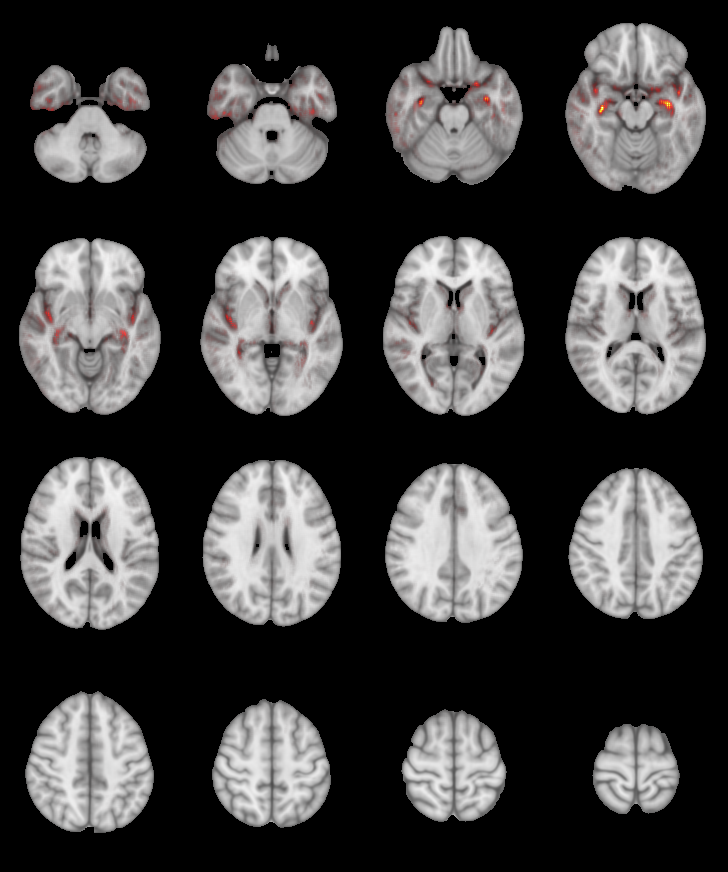
\includegraphics[
								width=\mriwidth,
								height=\mriheight,
								clip=true,
								trim = 192mm 232mm 0mm 0mm
							]{data/samples/subject3.png}
						}
					};

					\node[inner sep=0pt, outer sep=0pt] (literature) at \comparisonlocation{(0.6, -1.75)} {
						
\includegraphics[width=1cm]{data/icons/paper.png}
					};

					\node[inner sep=0pt, outer sep=0pt] (mean) at \comparisonlocation{(-0.6, 0)} {
						
\includegraphics[
							width=1cm,
							clip=true,
							trim = 192mm 232mm 0mm 0mm
						]{data/averages/dementia.png}
					};
					\node[inner sep=0pt, outer sep=0pt] (ale) at \comparisonlocation{(0.6, 0)} {
						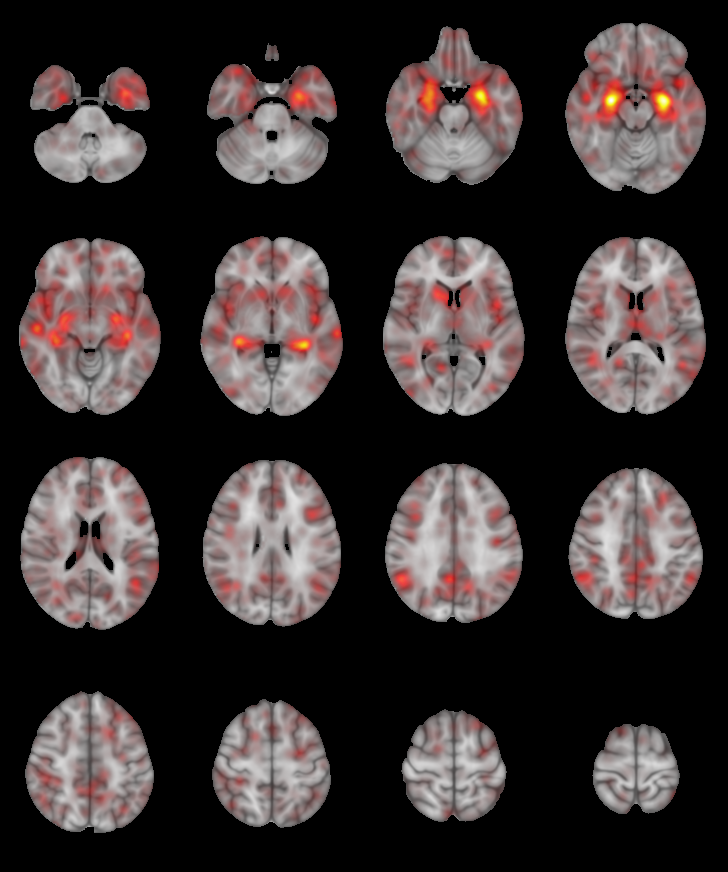
\includegraphics[
							width=1cm,
							clip=true,
							trim = 192mm 232mm 0mm 0mm
						]{data/averages/ALE.png}
					};

					\node[
						draw=black,
						minimum width=2.6cm,
						minimum height=1.5cm,
						outer sep=0pt,
						label={[label distance=-0.5mm]:{\scriptsize{Comparison}}}
					] (comparison) at \comparisonlocation{(0, 0)} {};

					\draw[
						color=outercolor,
						-\outerarrow,
						line width=0.1cm
					] (literature) to (ale);

					\draw[
						color=outercolor,
						-\outerarrow,
						line width=0.1cm
					] \patientlocation{(0.87, 0)} to (mean);

					\node[inner sep=0pt, outer sep=0pt] (results) at \resultslocation{(0, 0)} {
						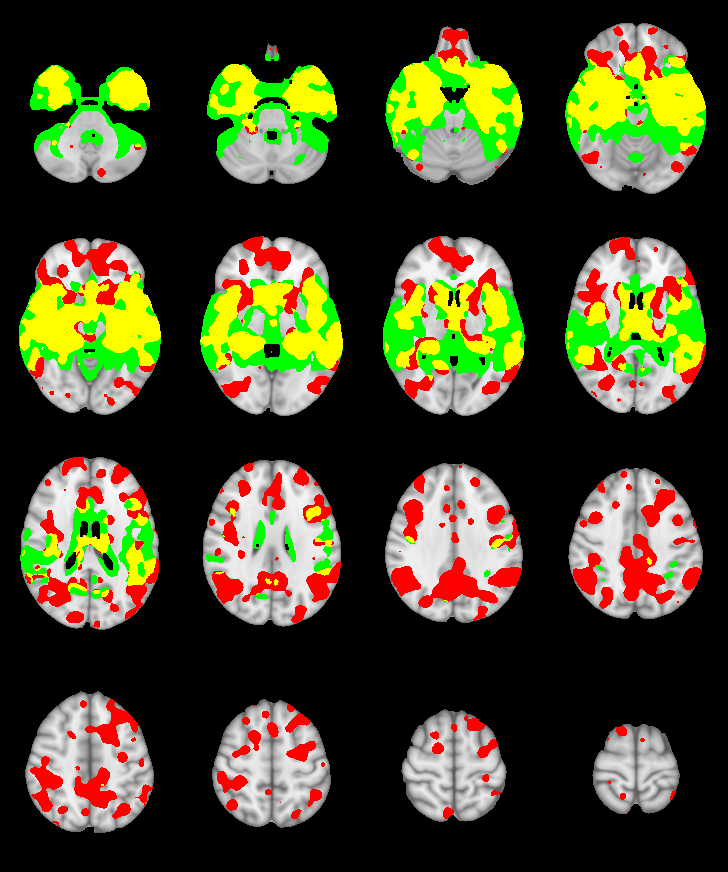
\includegraphics[
							width=1cm,
							clip=true,
							trim = 192mm 232mm 0mm 0mm
						]{data/overlap/test_70.png}
					};

					\node[
						minimum width=1.3cm,
						minimum height=0.85cm,
						draw=black
					] (overlap) at \resultslocation{(0, -1.2)} {};

					\fill[
						fill=cb-blue!30
					] ($ (overlap.north west) + (0.01, -0.03) $) to [out=-10, in=120] ($ (overlap.south east) + (-0.02, 0.01) $) to (overlap.south west) to (overlap.north west);

					\fill[
						pattern=north east lines,
						pattern color=white
					] ($ (overlap.north west) + (0.01, -0.03) $) to [out=-10, in=120] ($ (overlap.south east) + (-0.02, 0.01) $) to (overlap.south west) to (overlap.north west);

					\draw[very thick,cb-blue] ($ (overlap.north west) + (0.01, -0.03) $) to [out=-10, in=120] ($ (overlap.south east) + (-0.02, 0.01) $);

					\node[
						minimum width=1.3cm,
						minimum height=0.85cm,
						draw=black,
						label={below:\scriptsize{Similarity}}
					] (overlap) at \resultslocation{(0, -1.2)} {};
					\draw[
						color=outercolor,
						-\outerarrow,
						line width=0.1cm
					] (comparison) to (results);
				\end{tikzpicture}
			}
		}
		\newline
		\noindent
		\scalebox{0.4}{
			\hspace{3cm}
			\fbox{
				\begin{tikzpicture}
					\newcommand{\mrivsep}{0.75}
					\newcommand{\mrihsep}{0.6}
					\newcommand{\mriwidth}{0.55cm}
					\newcommand{\mriheight}{0.7cm}

					\node[anchor=north west] at (0, 0.25) {\footnotesize{4. Stratify participants with MCI using predictions and relevance maps}};
					\node[anchor=north east] at (\plotwidth, 0) {};

					\newcommand{\patientlocation}[1]{($ (0.5 * \plotwidth - 4, -1.7) + ####1 $)}
					\newcommand{\edalocation}[1]{($ (0.5 * \plotwidth, -2.2) + ####1 $)}
					\newcommand{\resultslocation}[1]{($ (0.5 * \plotwidth + 4, -1.7) + ####1 $)}

					\def\edaheight{1.5}

					\node[align=center, font=\scriptsize\linespread{0.85}\selectfont] at \patientlocation{(0, 1)} {MCI\\patients};

					\node[] at \patientlocation{(-1 * \mrihsep, -0.5*\mrivsep)} {
						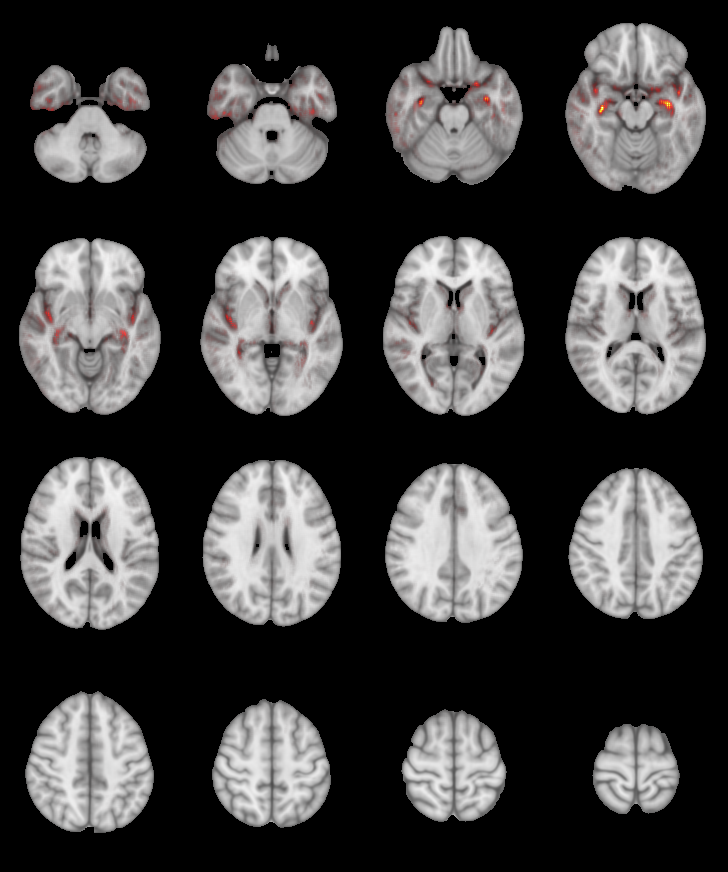
\includegraphics[
							width=\mriwidth,
							height=\mriheight,
							clip=true,
							trim = 128mm 232mm 64mm 0mm
						]{data/samples/subject3.png}
					};
					\node[] at \patientlocation{(0, -0.5*\mrivsep)} {
						\scalebox{-1}[1]{
							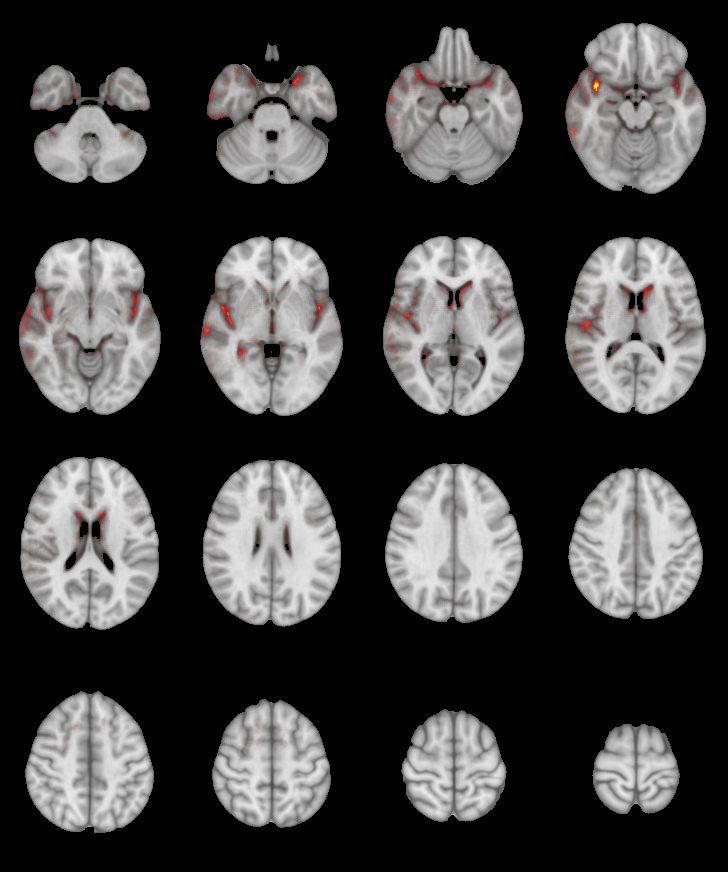
\includegraphics[
								width=\mriwidth,
								height=\mriheight,
								clip=true,
								trim = 192mm 232mm 0mm 0mm
							]{data/samples/subject2.png}
						}
					};
					\node[] at \patientlocation{(1 * \mrihsep, -0.5*\mrivsep)} {
						\scalebox{-1}[1]{
							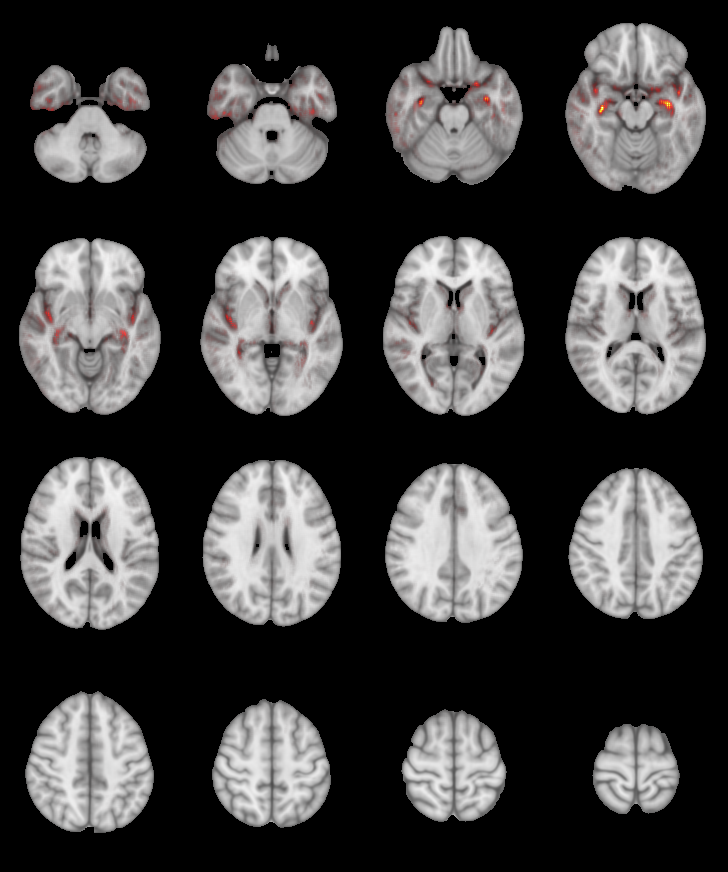
\includegraphics[
								width=\mriwidth,
								height=\mriheight,
								clip=true,
								trim = 0mm 154mm 192mm 78mm
							]{data/samples/subject3.png}
						}
					};
					\node[] at \patientlocation{(-1 * \mrihsep, 0.5*\mrivsep)} {
						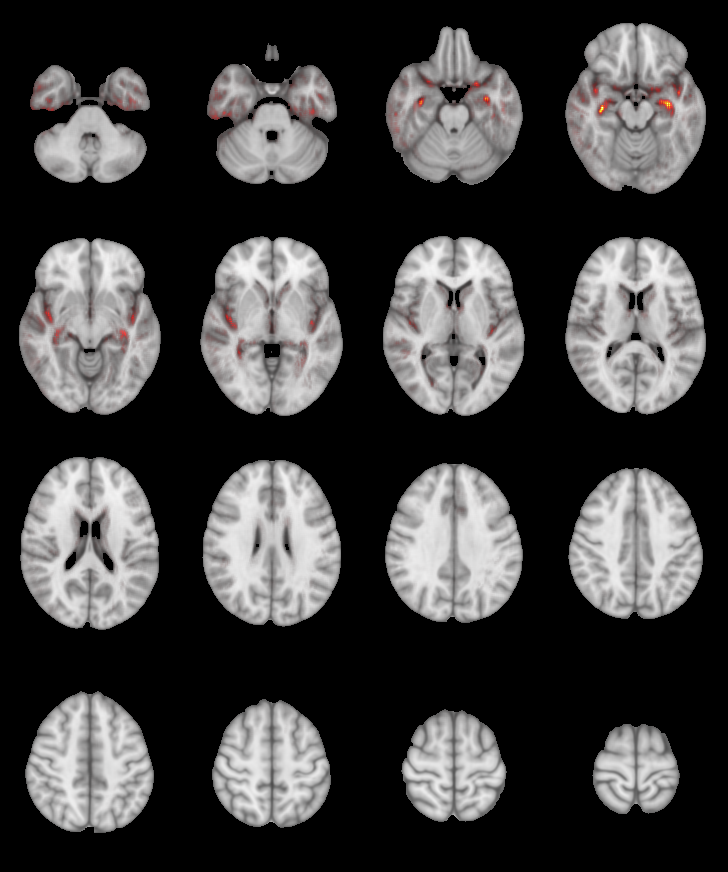
\includegraphics[
							width=\mriwidth,
							height=\mriheight,
							clip=true,
							trim = 192mm 232mm 0mm 0mm
						]{data/samples/subject3.png}
					};
					\node[] at \patientlocation{(0, 0.5*\mrivsep)} {
						\scalebox{-1}[1]{
							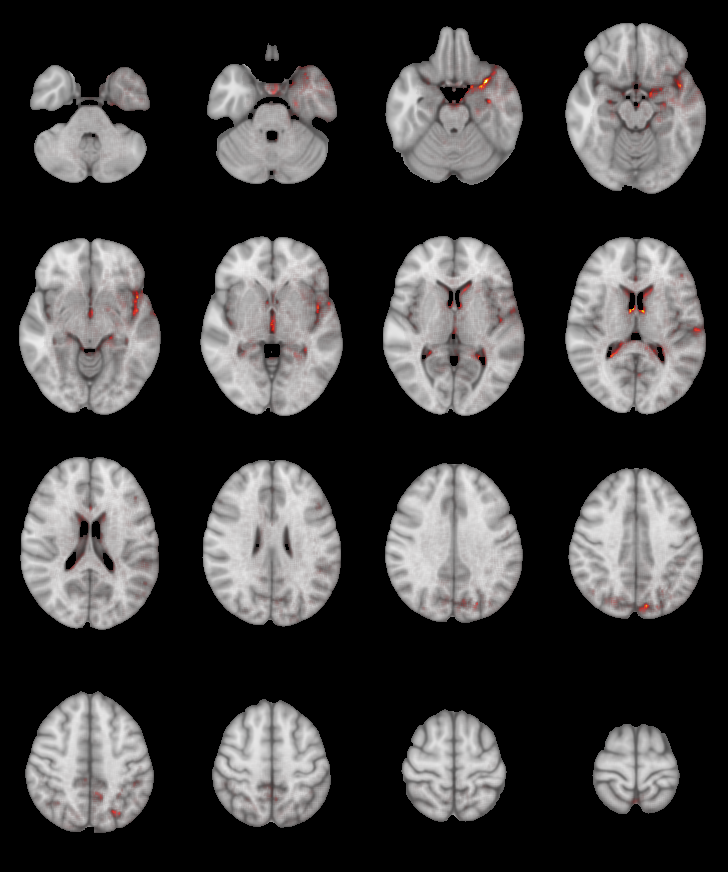
\includegraphics[
								width=\mriwidth,
								height=\mriheight,
								clip=true,
								trim = 64mm 232mm 128mm 0mm
							]{data/samples/subject1.png}
						}
					};
					\node[] at \patientlocation{(1 * \mrihsep, 0.5*\mrivsep)} {
						\scalebox{-1}[1]{
							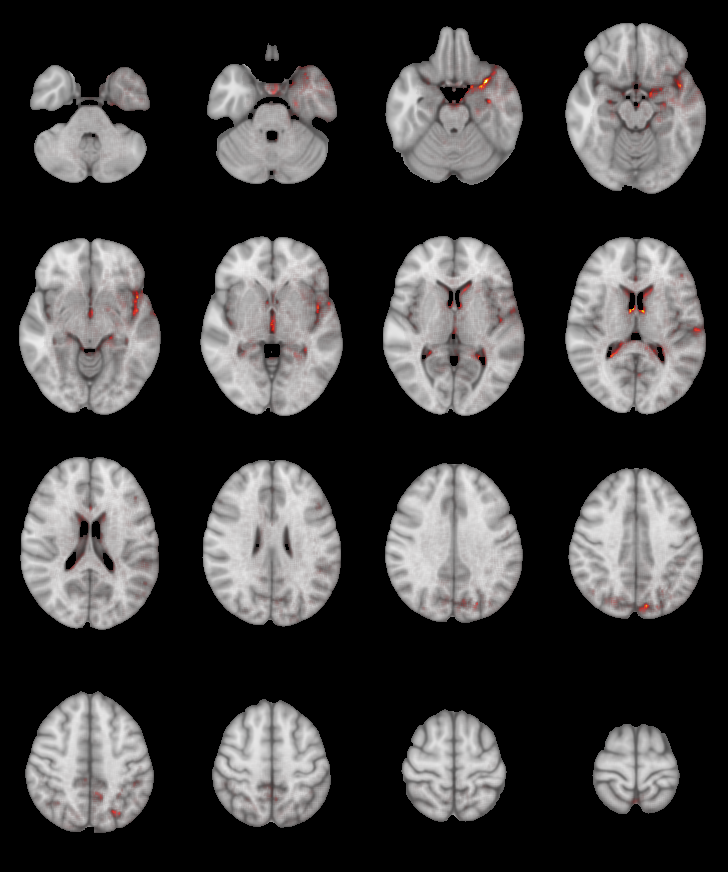
\includegraphics[
								width=\mriwidth,
								height=\mriheight,
								clip=true,
								trim = 192mm 154mm 0mm 78mm
							]{data/samples/subject1.png}
						}
					};


					\newcommand{\edapoint}[4]{
						\node[circle, minimum size=####4, draw=black, fill=####3, inner sep=0pt, outer sep=0pt] at \edalocation{(####1, ####2)} {};
					}

					\draw[->] \edalocation{(0, 0)} -- \edalocation{(0,\edaheight)};
					\draw[->] \edalocation{(0, 0)} -- \edalocation{(0.6*\edaheight, -0.3*\edaheight)};
					\draw[->] \edalocation{(0, 0)} -- \edalocation{(-0.6*\edaheight, -0.3*\edaheight)};

					\edapoint{0.35}{-0.15}{controls-default!50!cases-default!50}{3.5pt}
					\edapoint{-0.05}{-0.3}{controls-default!40!cases-default!60}{3.6pt}
					\edapoint{-0.15}{0.15}{controls-default!60!cases-default!40}{3.6pt}
					\edapoint{-0.1}{0.5}{controls-default!30!cases-default!70}{3.7pt}
					\edapoint{0.55}{0.15}{controls-default!20!cases-default!80}{3.75pt}
					\edapoint{-0.35}{0.15}{controls-default!70!cases-default!30}{3.8pt}
					\edapoint{-0.35}{-0.35}{controls-default!25!cases-default!75}{3.8pt}
					\edapoint{-0.3}{-0.05}{controls-default!75!cases-default!25}{3.8pt}
					\edapoint{0.3}{-0.3}{controls-default!30!cases-default!70}{3.9pt}
					\edapoint{0.2}{0.1}{controls-default!25!cases-default!75}{4pt}
					\edapoint{-0.4}{0.5}{controls-default!40!cases-default!60}{4pt}
					\edapoint{0.3}{0.05}{controls-default!65!cases-default!35}{4.05pt}
					\edapoint{0.1}{0.4}{controls-default!60!cases-default!40}{4.1pt}
					\edapoint{0.5}{0.4}{controls-default!75!cases-default!25}{4.1pt}
					\edapoint{0.5}{0.4}{controls-default!75!cases-default!25}{4.1pt}
					\edapoint{0.1}{-0.1}{controls-default!20!cases-default!80}{4.2pt}
					\edapoint{0.05}{0.7}{controls-default!10!cases-default!90}{4.3pt}
					\edapoint{-0.5}{-0.2}{controls-default!80!cases-default!20}{4.4pt}

					\newcommand\axisheight{1.5}
					\newcommand\axiswidth{2}
					\newcommand\axisorigo{\resultslocation{(-0.5 * \axiswidth, -0.5 * \axisheight)}}
					\newcommand\axisxmax{\resultslocation{(0.5 * \axiswidth, -0.5 * \axisheight)}}
					\newcommand\axisymax{\resultslocation{(-0.5 * \axiswidth, 0.5 * \axisheight)}}

					\draw[->] \axisorigo -- \axisxmax;
					\draw[->] \axisorigo -- \axisymax;

					\newcommand{\resultspoint}[4]{
						\node[circle, minimum size=4pt, draw=black, fill=controls-default!####3!cases-default!####4, inner sep=0pt, outer sep=0pt] at \resultslocation{(-0.5 * \axiswidth + ####1 * \axiswidth, -0.5 * \axisheight + ####2 * \axisheight)} {};
					}

					\resultspoint{0.6}{0.4}{50}{50}
					\resultspoint{0.4}{0.8}{40}{60}
					\resultspoint{0.15}{0.65}{60}{40}
					\resultspoint{0.45}{0.95}{30}{70}
					\resultspoint{1}{0.6}{20}{80}
					\resultspoint{0.3}{0.3}{70}{30}
					\resultspoint{0.2}{0.3}{75}{25}
					\resultspoint{0.8}{0.6}{30}{70}
					\resultspoint{0.65}{0.85}{25}{75}
					\resultspoint{0.65}{0.55}{40}{60}
					\resultspoint{0.25}{0.45}{65}{35}
					\resultspoint{0.45}{0.35}{60}{40}
					\resultspoint{0.10}{0.30}{75}{25}
					\resultspoint{0.35}{0.05}{75}{25}
					\resultspoint{0.9}{0.7}{20}{80}
					\resultspoint{0.95}{0.85}{10}{90}
					\resultspoint{0.25}{0.15}{80}{20}

					\draw[dashed] \resultslocation{(-0.5 * \axiswidth, 0.4 * \axisheight)} -- \resultslocation{(0.4 * \axiswidth, -0.5 * \axisheight)};
					\draw[dashed] \resultslocation{(0.25 * \axiswidth, 0.5 * \axisheight)} -- \resultslocation{(0.19 * \axiswidth, -0.5 * \axisheight)};

					\draw[
						color=outercolor,
						-\outerarrow,
						line width=0.1cm
					] \patientlocation{(0.87, 0)} to (0.5 * \plotwidth - 1, -1.7);

					\draw[
						color=outercolor,
						-\outerarrow,
						line width=0.1cm
					] (0.5 * \plotwidth + 1, -1.7) -- \resultslocation{(-0.5 * \axiswidth, 0)};
				\end{tikzpicture}
			}
		}
		\newline
		\noindent
	\end{frame}

	\begin{frame}{Case-control predictions} % Intro
		\centering
		\vfill
		\scalebox{0.8}{
			\fbox{
				\begin{tikzpicture}
					\newcommand{\mrivsep}{0.52}
					\newcommand{\mrihsep}{0.44}

					\node[anchor=north west] at (0, 0.1) {\footnotesize{1. Train binary classification CNNs to detect signs of dementia in structural MRIs}};
					\node[anchor=north east] at (\plotwidth, 0) {};

					\newcommand{\patientlocation}[1]{($ (1, -1.6) + ####1 $)}
					\newcommand{\controllocation}[1]{($ (1, -2.8) + ####1 $)}
					\newcommand{\modellocation}[1]{($ (0.5 * \plotwidth, -2.2) + ####1 $)}


					\node[anchor=south, align=center, font=\scriptsize\linespread{0.85}\selectfont] at \patientlocation{(0, 0.38)} {Dementia\\patients};
					\node[anchor=north] at \controllocation{(0, -0.40)} {\scriptsize{Controls}};

					\node[] at \patientlocation{(-1 * \mrihsep, -0.5*\mrivsep)} {
                    	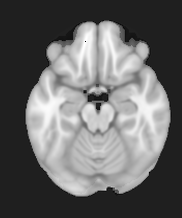
\includegraphics[height=0.5cm]{data/mris/slice_0.png}
					};
					\node[] at \patientlocation{(0, -0.5*\mrivsep)} {
						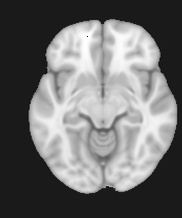
\includegraphics[height=0.5cm]{data/mris/slice_1.png}
					};
					\node[] at \patientlocation{(1 * \mrihsep, -0.5*\mrivsep)} {
						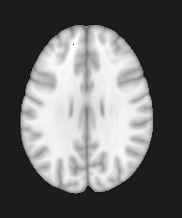
\includegraphics[height=0.5cm]{data/mris/slice_2.png}
					};
					\node[] at \patientlocation{(-1 * \mrihsep, 0.5*\mrivsep)} {
						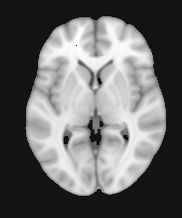
\includegraphics[height=0.5cm]{data/mris/slice_3.png}
					};
					\node[] at \patientlocation{(0, 0.5*\mrivsep)} {
						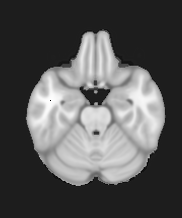
\includegraphics[height=0.5cm]{data/mris/slice_4.png}
					};
					\node[] at \patientlocation{(1 * \mrihsep, 0.5*\mrivsep)} {
						\includegraphics[height=0.5cm]{data/mris/slice_5.png}
					};

					\node[] at \controllocation{(-1 * \mrihsep, -0.5*\mrivsep)} {
						\includegraphics[height=0.5cm]{data/mris/slice_6.png}
					};
					\node[] at \controllocation{(0, -0.5*\mrivsep)} {
						\includegraphics[height=0.5cm]{data/mris/slice_7.png}
					};
					\node[] at \controllocation{(1 * \mrihsep, -0.5*\mrivsep)} {
						\includegraphics[height=0.5cm]{data/mris/slice_8.png}
					};
					\node[] at \controllocation{(-1 * \mrihsep, 0.5*\mrivsep)} {
						\includegraphics[height=0.5cm]{data/mris/slice_9.png}
					};
					\node[] at \controllocation{(0, 0.5*\mrivsep)} {
						\includegraphics[height=0.5cm]{data/mris/slice_10.png}
					};
					\node[] at \controllocation{(1 * \mrihsep, 0.5*\mrivsep)} {
						\includegraphics[height=0.5cm]{data/mris/slice_11.png}
					};
					\node[circle, inner sep=0pt, fill=none, outer sep=0pt, line width=0pt, draw=none] (n00) at \modellocation{(-3 * \hsep, 0)} {};

					\node[circle, minimum size=\nodesize, inner sep=0pt, fill=train-fill!35, outer sep=0pt, line width=0pt, draw=train-fill!35] (n10) at \modellocation{(-2 * \hsep, 2 * \vsep)} {};
					\node[circle, minimum size=\nodesize, inner sep=0pt, fill=train-fill, outer sep=0pt, line width=0pt, draw=train-fill] (n11) at \modellocation{(-2 * \hsep, 1 * \vsep)} {};
					\node[circle, minimum size=\nodesize, inner sep=0pt, fill=train-fill!15, outer sep=0pt, line width=0pt, draw=train-fill!15] (n12) at \modellocation{(-2 * \hsep, 0)} {};
					\node[circle, minimum size=\nodesize, inner sep=0pt, fill=train-fill!85, outer sep=0pt, line width=0pt, draw=train-fill!85] (n13) at \modellocation{(-2 * \hsep, -1 * \vsep)} {};
					\node[circle, minimum size=\nodesize, inner sep=0pt, fill=train-fill!90, outer sep=0pt, line width=0pt, draw=train-fill!90] (n14) at \modellocation{(-2 * \hsep, -2 * \vsep)} {};

					\node[circle, minimum size=\nodesize, inner sep=0pt, fill=train-fill!55, outer sep=0pt, line width=0pt, draw=train-fill!55] (n20) at \modellocation{(-1 * \hsep, 1.5 * \vsep)} {};
					\node[circle, minimum size=\nodesize, inner sep=0pt, fill=train-fill!20, outer sep=0pt, line width=0pt, draw=train-fill!20] (n21) at \modellocation{(-1 * \hsep, 0.5 * \vsep)} {};
					\node[circle, minimum size=\nodesize, inner sep=0pt, fill=train-fill!90, outer sep=0pt, line width=0pt, draw=train-fill!50] (n22) at \modellocation{(-1 * \hsep, -0.5 * \vsep)} {};
					\node[circle, minimum size=\nodesize, inner sep=0pt, fill=train-fill!35, outer sep=0pt, line width=0pt, draw=train-fill!35] (n23) at \modellocation{(-1 * \hsep, -1.5 * \vsep)} {};

					\node[circle, minimum size=\nodesize, inner sep=0pt, fill=train-fill!95, outer sep=0pt, line width=0pt, draw=train-fill!65] (n30) at \modellocation{(0 * \hsep, 1.5 * \vsep)} {};
					\node[circle, minimum size=\nodesize, inner sep=0pt, fill=train-fill!20, outer sep=0pt, line width=0pt, draw=train-fill!20] (n31) at \modellocation{(0 * \hsep, 0.5 * \vsep)} {};
					\node[circle, minimum size=\nodesize, inner sep=0pt, fill=train-fill!90, outer sep=0pt, line width=0pt, draw=train-fill!90] (n32) at \modellocation{(0 * \hsep, -0.5 * \vsep)} {};
					\node[circle, minimum size=\nodesize, inner sep=0pt, fill=train-fill!80, outer sep=0pt, line width=0pt, draw=train-fill!80] (n33) at \modellocation{(0 * \hsep, -1.5 * \vsep)} {};

					\node[circle, minimum size=\nodesize, inner sep=0pt, fill=train-fill!50, outer sep=0pt, line width=0pt, draw=train-fill!50] (n40) at \modellocation{(1 * \hsep, 1*\vsep)} {};
					\node[circle, minimum size=\nodesize, inner sep=0pt, fill=train-fill!90, outer sep=0pt, line width=0pt, draw=train-fill!70] (n41) at \modellocation{(1 * \hsep, 0*\vsep)} {};
					\node[circle, minimum size=\nodesize, inner sep=0pt, fill=train-fill!70, outer sep=0pt, line width=0pt, draw=train-fill!30] (n42) at \modellocation{(1 * \hsep, -1*\vsep)} {};

					\node[circle, minimum size=\nodesize, inner sep=0pt, fill=train-fill, outer sep=0pt, line width=0pt, draw=train-fill] (n50) at \modellocation{(2 * \hsep, 1*\vsep)} {};
					\node[circle, minimum size=\nodesize, inner sep=0pt, fill=train-fill!70, outer sep=0pt, line width=0pt, draw=train-fill!70] (n51) at \modellocation{(2 * \hsep, 0*\vsep)} {};
					\node[circle, minimum size=\nodesize, inner sep=0pt, fill=train-fill!30, outer sep=0pt, line width=0pt, draw=train-fill!30] (n52) at \modellocation{(2 * \hsep, -1*\vsep)} {};

					\node[circle, minimum size=\nodesize, inner sep=0pt, fill=train-fill!80, outer sep=0pt, line width=0pt, draw=train-fill!65] (n60) at \modellocation{(3 * \hsep, 0)} {};

					\node[] (loss) at (1+2*4.85, -2.2) {\scriptsize{$logloss(y, \hat{y})$}};

					\draw[
						color=train-fill!35,
						\innerarrow-\innerarrow,
						line width=\arrowwidth
					] (n00) to [out=20,in=200] (n10) {};
					\draw[
						color=train-fill,
						\innerarrow-\innerarrow,
						line width=\arrowwidth
					] (n00) to [out=10,in=190] (n11) {};
					\draw[
						color=train-fill!15,
						\innerarrow-\innerarrow,
						line width=\arrowwidth
					] (n00) to [out=0,in=180] (n12) {};
					\draw[
						color=train-fill!85,
						\innerarrow-\innerarrow,
						line width=\arrowwidth
					] (n00) to [out=-10,in=170] (n13) {};
					\draw[
						color=train-fill!90,
						\innerarrow-\innerarrow,
						line width=\arrowwidth
					] (n00) to [out=-20,in=160] (n14) {};

					\draw[
						color=train-fill!35,
						\innerarrow-\innerarrow,
						line width=\arrowwidth
					] (n10) to [out=-5,in=175] (n20) {};
					\draw[
						color=train-fill!10,
						\innerarrow-\innerarrow,
						line width=\arrowwidth
					] (n10) to [out=-15,in=165] (n21) {};
					\draw[
						color=train-fill!70,
						\innerarrow-\innerarrow,
						line width=\arrowwidth
					] (n10) to [out=-25,in=155] (n22) {};
					\draw[
						color=train-fill!50,
						\innerarrow-\innerarrow,
						line width=\arrowwidth
					] (n10) to [out=-35,in=145] (n23) {};

					\draw[
						color=train-fill!30,
						\innerarrow-\innerarrow,
						line width=\arrowwidth
					] (n11) to [out=5,in=185] (n20) {};
					\draw[
						color=train-fill!25,
						\innerarrow-\innerarrow,
						line width=\arrowwidth
					] (n11) to [out=-5,in=175] (n21) {};
					\draw[
						color=train-fill!95,
						\innerarrow-\innerarrow,
						line width=\arrowwidth
					] (n11) to [out=-15,in=165] (n22) {};
					\draw[
						color=train-fill!35,
						\innerarrow-\innerarrow,
						line width=\arrowwidth
					] (n11) to [out=-25,in=155] (n23) {};

					\draw[
						color=train-fill!70,
						\innerarrow-\innerarrow,
						line width=\arrowwidth
					] (n12) to [out=15,in=195] (n20) {};
					\draw[
						color=train-fill!20,
						\innerarrow-\innerarrow,
						line width=\arrowwidth
					] (n12) to [out=5,in=185] (n21) {};
					\draw[
						color=train-fill!80,
						\innerarrow-\innerarrow,
						line width=\arrowwidth
					] (n12) to [out=-5,in=175] (n22) {};
					\draw[
						color=train-fill,
						\innerarrow-\innerarrow,
						line width=\arrowwidth
					] (n12) to [out=-15,in=165] (n23) {};

					\draw[
						color=train-fill!40,
						\innerarrow-\innerarrow,
						line width=\arrowwidth
					] (n13) to [out=25,in=205] (n20) {};
					\draw[
						color=train-fill!35,
						\innerarrow-\innerarrow,
						line width=\arrowwidth
					] (n13) to [out=15,in=195] (n21) {};
					\draw[
						color=train-fill!20,
						\innerarrow-\innerarrow,
						line width=\arrowwidth
					] (n13) to [out=5,in=185] (n22) {};
					\draw[
						color=white,
						\innerarrow-\innerarrow,
						line width=\arrowwidth
					] (n13) to [out=-5,in=175] (n23) {};

					\draw[
						color=train-fill!40,
						\innerarrow-\innerarrow,
						line width=\arrowwidth
					] (n14) to [out=35,in=215] (n20) {};
					\draw[
						color=train-fill!85,
						\innerarrow-\innerarrow,
						line width=\arrowwidth
					] (n14) to [out=25,in=205] (n21) {};
					\draw[
						color=train-fill!35,
						\innerarrow-\innerarrow,
						line width=\arrowwidth
					] (n14) to [out=15,in=195] (n22) {};
					\draw[
						color=train-fill,
						\innerarrow-\innerarrow,
						line width=\arrowwidth
					] (n14) to [out=5,in=185] (n23) {};

					\draw[
						color=train-fill!85,
						\innerarrow-\innerarrow,
						line width=\arrowwidth
					] (n20) to [out=0,in=180] (n30) {};
					\draw[
						color=train-fill!50,
						\innerarrow-\innerarrow,
						line width=\arrowwidth
					] (n20) to [out=-10,in=170] (n31) {};
					\draw[
						color=train-fill!75,
						\innerarrow-\innerarrow,
						line width=\arrowwidth
					] (n20) to [out=-20,in=160] (n32) {};
					\draw[
						color=white,
						\innerarrow-\innerarrow,
						line width=\arrowwidth
					] (n20) to [out=-30,in=150] (n33) {};

					\draw[
						color=train-fill,
						\innerarrow-\innerarrow,
						line width=\arrowwidth
					] (n21) to [out=10,in=190] (n30) {};
					\draw[
						color=train-fill!30,
						\innerarrow-\innerarrow,
						line width=\arrowwidth
					] (n21) to [out=0,in=180] (n31) {};
					\draw[
						color=train-fill!25,
						\innerarrow-\innerarrow,
						line width=\arrowwidth
					] (n21) to [out=-10,in=170] (n32) {};
					\draw[
						color=white,
						\innerarrow-\innerarrow,
						line width=\arrowwidth
					] (n21) to [out=-20,in=160] (n33) {};

					\draw[
						color=train-fill!35,
						\innerarrow-\innerarrow,
						line width=\arrowwidth
					] (n22) to [out=20,in=200] (n30) {};
					\draw[
						color=train-fill!95,
						\innerarrow-\innerarrow,
						line width=\arrowwidth
					] (n22) to [out=10,in=190] (n31) {};
					\draw[
						color=train-fill!80,
						\innerarrow-\innerarrow,
						line width=\arrowwidth
					] (n22) to [out=0,in=180] (n32) {};
					\draw[
						color=white,
						\innerarrow-\innerarrow,
						line width=\arrowwidth
					] (n22) to [out=-10,in=170] (n33) {};

					\draw[
						color=train-fill!45,
						\innerarrow-\innerarrow,
						line width=\arrowwidth
					] (n23) to [out=30,in=210] (n30) {};
					\draw[
						color=train-fill!70,
						\innerarrow-\innerarrow,
						line width=\arrowwidth
					] (n23) to [out=20,in=200] (n31) {};
					\draw[
						color=train-fill!10,
						\innerarrow-\innerarrow,
						line width=\arrowwidth
					] (n23) to [out=10,in=190] (n32) {};
					\draw[
						color=train-fill!20,
						\innerarrow-\innerarrow,
						line width=\arrowwidth
					] (n23) to [out=0,in=180] (n33) {};

					\draw[
						color=train-fill!50,
						\innerarrow-\innerarrow,
						line width=\arrowwidth
					] (n30) to [out=-5,in=175] (n40) {};
					\draw[
						color=train-fill!30,
						\innerarrow-\innerarrow,
						line width=\arrowwidth
					] (n30) to [out=-15,in=165] (n41) {};
					\draw[
						color=train-fill,
						\innerarrow-\innerarrow,
						line width=\arrowwidth
					] (n30) to [out=-25,in=155] (n42) {};

					\draw[
						color=train-fill!45,
						\innerarrow-\innerarrow,
						line width=\arrowwidth
					] (n31) to [out=5,in=185] (n40) {};
					\draw[
						color=train-fill!90,
						\innerarrow-\innerarrow,
						line width=\arrowwidth
					] (n31) to [out=-5,in=175] (n41) {};
					\draw[
						color=train-fill!45,
						\innerarrow-\innerarrow,
						line width=\arrowwidth
					] (n31) to [out=-15,in=165] (n42) {};

					\draw[
						color=train-fill!15,
						\innerarrow-\innerarrow,
						line width=\arrowwidth
					] (n32) to [out=15,in=195] (n40) {};
					\draw[
						color=train-fill!70,
						\innerarrow-\innerarrow,
						line width=\arrowwidth
					] (n32) to [out=5,in=185] (n41) {};
					\draw[
						color=train-fill!50,
						\innerarrow-\innerarrow,
						line width=\arrowwidth
					] (n32) to [out=-5,in=175] (n42) {};

					\draw[
						color=train-fill!40,
						\innerarrow-\innerarrow,
						line width=\arrowwidth
					] (n33) to [out=25,in=205] (n40) {};
					\draw[
						color=train-fill!20,
						\innerarrow-\innerarrow,
						line width=\arrowwidth
					] (n33) to [out=15,in=195] (n41) {};
					\draw[
						color=train-fill!90,
						\innerarrow-\innerarrow,
						line width=\arrowwidth
					] (n33) to [out=5,in=185] (n42) {};

					\draw[
						color=train-fill!25,
						\innerarrow-\innerarrow,
						line width=\arrowwidth
					] (n40) to [out=0,in=180] (n50) {};
					\draw[
						color=train-fill!15,
						\innerarrow-\innerarrow,
						line width=\arrowwidth
					] (n40) to [out=-10,in=170] (n51) {};
					\draw[
						color=train-fill,
						\innerarrow-\innerarrow,
						line width=\arrowwidth
					] (n40) to [out=-20,in=160] (n52) {};

					\draw[
						color=train-fill!35,
						\innerarrow-\innerarrow,
						line width=\arrowwidth
					] (n41) to [out=10,in=190] (n50) {};
					\draw[
						color=train-fill!10,
						\innerarrow-\innerarrow,
						line width=\arrowwidth
					] (n41) to [out=0,in=180] (n51) {};
					\draw[
						color=train-fill!90,
						\innerarrow-\innerarrow,
						line width=\arrowwidth
					] (n41) to [out=-10,in=170] (n52) {};

					\draw[
						color=train-fill!50,
						\innerarrow-\innerarrow,
						line width=\arrowwidth
					] (n42) to [out=20,in=200] (n50) {};
					\draw[
						color=train-fill!40,
						\innerarrow-\innerarrow,
						line width=\arrowwidth
					] (n42) to [out=10,in=190] (n51) {};
					\draw[
						color=train-fill!20,
						\innerarrow-\innerarrow,
						line width=\arrowwidth
					] (n42) to [out=0,in=180] (n52) {};

					\draw[
						color=train-fill!80,
						\innerarrow-\innerarrow,
						line width=\arrowwidth,
					] (n50) to [out=-10,in=170] (n60) {};
					\draw[
						color=train-fill!90,
						\innerarrow-\innerarrow,
						line width=\arrowwidth,
					] (n51) to [out=0,in=180] (n60) {};
					\draw[
						color=train-fill!30,
						\innerarrow-\innerarrow,
						line width=\arrowwidth,
					] (n52) to [out=10,in=190] (n60) {};

					\draw[black] (n00.center) --
								($ (n00) + (0, 2*\vsep+0.5*\nodesize+2pt) $) --
								($ (n00) + (6*\hsep+0.5*\nodesize+2pt, 2*\vsep+0.5*\nodesize+2pt) $) --
								($ (n00) + (6*\hsep+0.5*\nodesize+2pt, -2*\vsep-0.5*\nodesize-2pt) $) --
								($ (n00) + (0, -2*\vsep-0.5*\nodesize-2pt) $) --
								(n00.center);

					\node[] at ($ (n30) + (0, \vsep+0.5*\nodesize) $) {\scriptsize{CNN}};

					\draw[
						color=outercolor,
						-\outerarrow,
						line width=0.1cm
					] \patientlocation{(0.65, 0)} to [out=0,in=180] (n00) {};
					\draw[
						color=outercolor,
						-\outerarrow,
						line width=0.1cm
					] \controllocation{(0.65, 0)} to [out=0,in=180] (n00) {};
					\draw[
						color=outercolor,
						\outerarrow-\outerarrow,
						line width=0.1cm
					] (n60) to [out=0,in=180] (loss) {};
				\end{tikzpicture}
			}
		}
		\vfill
	\end{frame}

	\begin{frame}{Case-control predictions} % Overall
		\centering
		\pgfplotstableread[col sep=comma]{data/predictions/test_distributions.csv}\testdistributions
		\pgfplotstableread[col sep=comma]{data/predictions/test_predictions.csv}\testpredictions
		\pgfplotstableread[col sep=comma]{data/predictions/test_auc.csv}\testauc

		\newcommand{\ymin}{-0.35}
		\newcommand{\ymax}{1.05}
		\colorlet{roc-curve}{cb-blue-purple}
		\newcommand{\length}{0.85\textwidth}
		\newcommand{\tx}{0.117}
		\newcommand{\ty}{0.816}

		\begin{figure}[t]
			\begin{subfigure}{\textwidth}
				\begin{tikzpicture}
					\begin{axis}[
						name=distributions,
						height=0.35\textwidth,
						width=0.945\textwidth,
						xtick pos=bottom,
						ymajorticks=false,
						xmin=0,
						xmax=1,
						ymin=\ymin,
						ymax=\ymax,
						xlabel=\footnotesize{Prediction},
						every tick label/.append style={font=\footnotesize}
					]
						\addplot[name path=controls, draw=controls-default, very thick] table [x=prediction,y=controls]{\testdistributions};
						\addplot[name path=cases, draw=cases-default, very thick] table [x=prediction,y=cases]{\testdistributions};
						\addplot[name path=zero, draw=black] coordinates {(0,0) (1,0)};
						\addplot[fill=controls-default, opacity=0.2] fill between [of=zero and controls];
						\addplot[fill=cases-default, opacity=0.2] fill between [of=zero and cases];
						\addplot[
							scatter/classes={
								control={controls-default, draw=black, opacity=0.5},
								case={cases-default, draw=black, opacity=0.5}
							},
							scatter,
							mark=*,
							only marks,
							point meta=explicit symbolic
						] table [
							y expr=\thisrow{y} * -0.15 - 0.1,
							meta=class,
							each nth point=\N
						] {\testpredictions};
						\addplot[dashed] coordinates {(0.5, \ymin) (0.5, \ymax)};
					\end{axis}
					% ONLY FOR ALIGNMENT
					\node[anchor=south east] at ($ (distributions.south west) + (-0.72,0.28) $) {};

					\node[anchor=south west] at ($ (distributions.south east) + (0,0.23) $) {\tiny{Controls}};
					\node[anchor=south west] at ($ (distributions.south east) + (0,-0.05) $) {\tiny{Cases}};
					\node[anchor=south,align=center] at (distributions.north) {\tiny{$t$}};
				\end{tikzpicture}
			\end{subfigure}
			\begin{subfigure}{0.49\textwidth}
				\hspace*{0.32cm}
				\centering
				\begin{tikzpicture}
					\begin{axis}[
						height=\length,
						width=\length,
						xtick pos=bottom,
						ytick pos=left,
						xtick={0.5, 1, \tx},
						ytick={0.5, 1, \ty},
						xmin=-0,
						xmax=1,
						ymin=0,
						ymax=1,
						xlabel=\footnotesize{FPR},
						ylabel=\footnotesize{TPR},
						every tick label/.append style={font=\footnotesize}
					]
						\addplot[dotted] coordinates {(\tx, 0) (\tx, 1)};
						\addplot[dotted] coordinates {(0, \ty) (1, \ty)};
						\addplot[draw=roc-curve,very thick] table [x=fpr,y=tpr] {\testauc};
						\addplot[] coordinates {(0,0) (1,1)};
						\node[anchor=south east, inner sep=5pt] at (axis cs: 1, 0) {\textbf{\footnotesize{AUC: 0.908}}};
						\node[
							name=threshold,
							draw=black,
							fill=roc-curve,
							star,
							star points=5,
							inner sep=0cm,
							minimum height=0.1cm,
							minimum width=0.2cm
						] at (axis cs: \tx, \ty) {};
						\node[anchor=north west] at (threshold.east) {\tiny{$t=0.5$}};
					\end{axis}
				\end{tikzpicture}
			\end{subfigure}
			\begin{subfigure}{0.49\textwidth}
				\hspace*{0.35cm}
				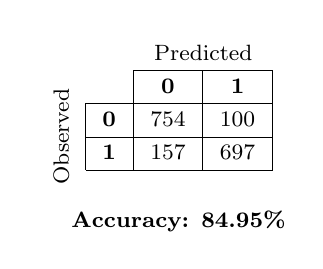
\begin{tikzpicture}
					\node[] at (0, 0) {
						\begin{tabular}{c|c|c|c|}
							\multicolumn{2}{c}{} & \multicolumn{2}{c}{\footnotesize{Predicted}} \\
							\cline{3-4}
							\multicolumn{1}{l}{\parbox[t]{2mm}{\multirow{4}{*}{\rotatebox[origin=c]{90}{\footnotesize{Observed}}}}} & \multicolumn{1}{c|}{} & \footnotesize{\textbf{0}} & \footnotesize{\textbf{1}} \\
							\cline{2-4}
							&\footnotesize{\textbf{0}}&\footnotesize{754}&\footnotesize{100}\\
							\cline{2-4}
							&\footnotesize{\textbf{1}}&\footnotesize{157}&\footnotesize{697}\\
							\cline{2-4}
						\end{tabular}
					};
					\node[] at (0.3, -1.5) {
						\textbf{\footnotesize{Accuracy: 84.95\%}}
					};
				\end{tikzpicture}
				\vspace*{0.6cm}
			\end{subfigure}
		\end{figure}\label{fig:test_predictions}
	\end{frame}

	\begin{frame}{Generating relevance maps} % Intro
		\centering
		\vfill
		\scalebox{0.8}{
			\fbox{
				\begin{tikzpicture}
					\newcommand{\mrivsep}{0.52}
					\newcommand{\mrihsep}{0.44}

					\node[anchor=north west] at (0, 0.1) {\footnotesize{2. Apply model and LRP for individual-level predictions and relevance maps}};
					\node[anchor=north east] at (\plotwidth, 0) {};

					\newcommand{\mrilocation}[1]{($ (1, -2.2) + ####1 $)}
					\newcommand{\modellocation}[1]{($ (0.5 * \plotwidth, -2.2) + ####1 $)}
					\newcommand{\lrplocation}[1]{($ (0.5 * \plotwidth, -5.2) + ####1 $)}
					\def\maplocation{(1, -5.2)}

					\node[anchor=south, align=center, font=\scriptsize\linespread{0.85}\selectfont] at \mrilocation{(0, 0.92)} {All\\subjects};

					\newcommand{\mrialpha}{0.2}
					\colorlet{predict-fill}{cb-blue}
					\colorlet{lrp-fill}{red}

					\node[] at \mrilocation{(-1 * \mrihsep, -1.5*\mrivsep)} {
						{\transparent{\mrialpha}\includegraphics[height=0.5cm]{data/mris/slice_5.png}}
					};
					\node[] at \mrilocation{(0, -1.5*\mrivsep)} {
						{\transparent{\mrialpha}\includegraphics[height=0.5cm]{data/mris/slice_7.png}}
					};
					\node[] at \mrilocation{(1 * \mrihsep, -1.5*\mrivsep)} {
						{\transparent{\mrialpha}\includegraphics[height=0.5cm]{data/mris/slice_11.png}}
					};
					\node[] at \mrilocation{(-1 * \mrihsep, -0.5*\mrivsep)} {
						{\transparent{\mrialpha}\includegraphics[height=0.5cm]{data/mris/slice_1.png}}
					};
					\node[] at \mrilocation{(0, -0.5*\mrivsep)} {
						{\transparent{\mrialpha}\includegraphics[height=0.5cm]{data/mris/slice_3.png}}
					};
					\node[inner sep=0pt, outer sep=0pt] (input) at \mrilocation{(1 * \mrihsep, -0.5*\mrivsep)} {
						\includegraphics[height=0.5cm]{data/mris/slice_4.png}
					};
					\node[] at \mrilocation{(-1 * \mrihsep, 0.5*\mrivsep)} {
						{\transparent{\mrialpha}\includegraphics[height=0.5cm]{data/mris/slice_2.png}}
					};
					\node[] at \mrilocation{(0, 0.5*\mrivsep)} {
						{\transparent{\mrialpha}\includegraphics[height=0.5cm]{data/mris/slice_0.png}}
					};
					\node[] at \mrilocation{(1 * \mrihsep, 0.5*\mrivsep)} {
						{\transparent{\mrialpha}\includegraphics[height=0.5cm]{data/mris/slice_10.png}}
					};
					\node[] at \mrilocation{(-1 * \mrihsep, 1.5*\mrivsep)} {
						{\transparent{\mrialpha}\includegraphics[height=0.5cm]{data/mris/slice_9.png}}
					};
					\node[] at \mrilocation{(0, 1.5*\mrivsep)} {
						{\transparent{\mrialpha}\includegraphics[height=0.5cm]{data/mris/slice_8.png}}
					};
					\node[] at \mrilocation{(1 * \mrihsep, 1.5*\mrivsep)} {
						{\transparent{\mrialpha}\includegraphics[height=0.5cm]{data/mris/slice_6.png}}
					};

					\node[circle, inner sep=0pt, fill=none, outer sep=0pt, line width=0pt, draw=none] (n00) at \modellocation{(-3 * \hsep, 0)} {};

					\node[circle, minimum size=\nodesize, inner sep=0pt, fill=predict-fill!85, outer sep=0pt, line width=0pt, draw=predict-fill!85] (n10) at \modellocation{(-2 * \hsep, 2 * \vsep)} {};
					\node[circle, minimum size=\nodesize, inner sep=0pt, fill=predict-fill, outer sep=0pt, line width=0pt, draw=predict-fill] (n11) at \modellocation{(-2 * \hsep, 1 * \vsep)} {};
					\node[circle, minimum size=\nodesize, inner sep=0pt, fill=predict-fill!75, outer sep=0pt, line width=0pt, draw=predict-fill!75] (n12) at \modellocation{(-2 * \hsep, 0)} {};
					\node[circle, minimum size=\nodesize, inner sep=0pt, fill=predict-fill!15, outer sep=0pt, line width=0pt, draw=predict-fill!15] (n13) at \modellocation{(-2 * \hsep, -1 * \vsep)} {};
					\node[circle, minimum size=\nodesize, inner sep=0pt, fill=predict-fill!50, outer sep=0pt, line width=0pt, draw=predict-fill!50] (n14) at \modellocation{(-2 * \hsep, -2 * \vsep)} {};

					\node[circle, minimum size=\nodesize, inner sep=0pt, fill=predict-fill!15, outer sep=0pt, line width=0pt, draw=predict-fill!15] (n20) at \modellocation{(-1 * \hsep, 1.5 * \vsep)} {};
					\node[circle, minimum size=\nodesize, inner sep=0pt, fill=predict-fill!65, outer sep=0pt, line width=0pt, draw=predict-fill!65] (n21) at \modellocation{(-1 * \hsep, 0.5 * \vsep)} {};
					\node[circle, minimum size=\nodesize, inner sep=0pt, fill=predict-fill!90, outer sep=0pt, line width=0pt, draw=predict-fill!90] (n22) at \modellocation{(-1 * \hsep, -0.5 * \vsep)} {};
					\node[circle, minimum size=\nodesize, inner sep=0pt, fill=predict-fill!40, outer sep=0pt, line width=0pt, draw=predict-fill!40] (n23) at \modellocation{(-1 * \hsep, -1.5 * \vsep)} {};

					\node[circle, minimum size=\nodesize, inner sep=0pt, fill=predict-fill!80, outer sep=0pt, line width=0pt, draw=predict-fill!80] (n30) at \modellocation{(0 * \hsep, 1.5 * \vsep)} {};
					\node[circle, minimum size=\nodesize, inner sep=0pt, fill=predict-fill!55, outer sep=0pt, line width=0pt, draw=predict-fill!55] (n31) at \modellocation{(0 * \hsep, 0.5 * \vsep)} {};
					\node[circle, minimum size=\nodesize, inner sep=0pt, fill=predict-fill!15, outer sep=0pt, line width=0pt, draw=predict-fill!15] (n32) at \modellocation{(0 * \hsep, -0.5 * \vsep)} {};
					\node[circle, minimum size=\nodesize, inner sep=0pt, fill=predict-fill!75, outer sep=0pt, line width=0pt, draw=predict-fill!75] (n33) at \modellocation{(0 * \hsep, -1.5 * \vsep)} {};

					\node[circle, minimum size=\nodesize, inner sep=0pt, fill=predict-fill, outer sep=0pt, line width=0pt, draw=predict-fill] (n40) at \modellocation{(1 * \hsep, 1*\vsep)} {};
					\node[circle, minimum size=\nodesize, inner sep=0pt, fill=predict-fill!20, outer sep=0pt, line width=0pt, draw=predict-fill!20] (n41) at \modellocation{(1 * \hsep, 0*\vsep)} {};
					\node[circle, minimum size=\nodesize, inner sep=0pt, fill=predict-fill!15, outer sep=0pt, line width=0pt, draw=predict-fill!15] (n42) at \modellocation{(1 * \hsep, -1*\vsep)} {};

					\node[circle, minimum size=\nodesize, inner sep=0pt, fill=predict-fill!75, outer sep=0pt, line width=0pt, draw=predict-fill!75] (n50) at \modellocation{(2 * \hsep, 1*\vsep)} {};
					\node[circle, minimum size=\nodesize, inner sep=0pt, fill=predict-fill!35, outer sep=0pt, line width=0pt, draw=predict-fill!35] (n51) at \modellocation{(2 * \hsep, 0*\vsep)} {};
					\node[circle, minimum size=\nodesize, inner sep=0pt, fill=predict-fill!65, outer sep=0pt, line width=0pt, draw=predict-fill!65] (n52) at \modellocation{(2 * \hsep, -1*\vsep)} {};

					\node[circle, minimum size=\nodesize, inner sep=0pt, fill=predict-fill!85, outer sep=0pt, line width=0pt, draw=predict-fill!85] (output) at \modellocation{(3 * \hsep, 0)} {};

					\node[] (diagnosis) at (1+2*4.85, -2.2) {\scriptsize{$\widehat{diagnosis}$}};

					\draw[
						color=predict-fill!85,
						-\innerarrow,
						line width=\arrowwidth
					] (n00) to [out=20,in=200] (n10) {};
					\draw[
						color=predict-fill,
						-\innerarrow,
						line width=\arrowwidth
					] (n00) to [out=10,in=190] (n11) {};
					\draw[
						color=predict-fill!75,
						-\innerarrow,
						line width=\arrowwidth
					] (n00) to [out=0,in=180] (n12) {};
					\draw[
						color=predict-fill!15,
						-\innerarrow,
						line width=\arrowwidth
					] (n00) to [out=-10,in=170] (n13) {};
					\draw[
						color=predict-fill!50,
						-\innerarrow,
						line width=\arrowwidth
					] (n00) to [out=-20,in=160] (n14) {};

					\draw[
						color=predict-fill!75,
						-\innerarrow,
						line width=\arrowwidth
					] (n10) to [out=-5,in=175] (n20) {};
					\draw[
						color=predict-fill!50,
						-\innerarrow,
						line width=\arrowwidth
					] (n10) to [out=-15,in=165] (n21) {};
					\draw[
						color=predict-fill!55,
						-\innerarrow,
						line width=\arrowwidth
					] (n10) to [out=-25,in=155] (n22) {};
					\draw[
						color=predict-fill!85,
						-\innerarrow,
						line width=\arrowwidth
					] (n10) to [out=-35,in=145] (n23) {};

					\draw[
						color=predict-fill!45,
						-\innerarrow,
						line width=\arrowwidth
					] (n11) to [out=5,in=185] (n20) {};
					\draw[
						color=predict-fill!50,
						-\innerarrow,
						line width=\arrowwidth
					] (n11) to [out=-5,in=175] (n21) {};
					\draw[
						color=predict-fill,
						-\innerarrow,
						line width=\arrowwidth
					] (n11) to [out=-15,in=165] (n22) {};
					\draw[
						color=predict-fill!15,
						-\innerarrow,
						line width=\arrowwidth
					] (n11) to [out=-25,in=155] (n23) {};

					\draw[
						color=predict-fill!35,
						-\innerarrow,
						line width=\arrowwidth
					] (n12) to [out=15,in=195] (n20) {};
					\draw[
						color=predict-fill!90,
						-\innerarrow,
						line width=\arrowwidth
					] (n12) to [out=5,in=185] (n21) {};
					\draw[
						color=predict-fill!80,
						-\innerarrow,
						line width=\arrowwidth
					] (n12) to [out=-5,in=175] (n22) {};
					\draw[
						color=predict-fill!20,
						-\innerarrow,
						line width=\arrowwidth
					] (n12) to [out=-15,in=165] (n23) {};

					\draw[
						color=predict-fill!55,
						-\innerarrow,
						line width=\arrowwidth
					] (n13) to [out=25,in=205] (n20) {};
					\draw[
						color=predict-fill!65,
						-\innerarrow,
						line width=\arrowwidth
					] (n13) to [out=15,in=195] (n21) {};
					\draw[
						color=predict-fill!35,
						-\innerarrow,
						line width=\arrowwidth
					] (n13) to [out=5,in=185] (n22) {};
					\draw[
						color=predict-fill!45,
						-\innerarrow,
						line width=\arrowwidth
					] (n13) to [out=-5,in=175] (n23) {};

					\draw[
						color=predict-fill!10,
						-\innerarrow,
						line width=\arrowwidth
					] (n14) to [out=35,in=215] (n20) {};
					\draw[
						color=predict-fill!90,
						-\innerarrow,
						line width=\arrowwidth
					] (n14) to [out=25,in=205] (n21) {};
					\draw[
						color=predict-fill!80,
						-\innerarrow,
						line width=\arrowwidth
					] (n14) to [out=15,in=195] (n22) {};
					\draw[
						color=predict-fill!35,
						-\innerarrow,
						line width=\arrowwidth
					] (n14) to [out=5,in=185] (n23) {};

					\draw[
						color=predict-fill!75,
						-\innerarrow,
						line width=\arrowwidth
					] (n20) to [out=0,in=180] (n30) {};
					\draw[
						color=predict-fill!50,
						-\innerarrow,
						line width=\arrowwidth
					] (n20) to [out=-10,in=170] (n31) {};
					\draw[
						color=predict-fill!85,
						-\innerarrow,
						line width=\arrowwidth
					] (n20) to [out=-20,in=160] (n32) {};
					\draw[
						color=predict-fill!45,
						-\innerarrow,
						line width=\arrowwidth
					] (n20) to [out=-30,in=150] (n33) {};

					\draw[
						color=predict-fill!20,
						-\innerarrow,
						line width=\arrowwidth
					] (n21) to [out=10,in=190] (n30) {};
					\draw[
						color=predict-fill!35,
						-\innerarrow,
						line width=\arrowwidth
					] (n21) to [out=0,in=180] (n31) {};
					\draw[
						color=predict-fill!15,
						-\innerarrow,
						line width=\arrowwidth
					] (n21) to [out=-10,in=170] (n32) {};
					\draw[
						color=predict-fill!90,
						-\innerarrow,
						line width=\arrowwidth
					] (n21) to [out=-20,in=160] (n33) {};

					\draw[
						color=predict-fill!65,
						-\innerarrow,
						line width=\arrowwidth
					] (n22) to [out=20,in=200] (n30) {};
					\draw[
						color=predict-fill!20,
						-\innerarrow,
						line width=\arrowwidth
					] (n22) to [out=10,in=190] (n31) {};
					\draw[
						color=predict-fill!30,
						-\innerarrow,
						line width=\arrowwidth
					] (n22) to [out=0,in=180] (n32) {};
					\draw[
						color=predict-fill!40,
						-\innerarrow,
						line width=\arrowwidth
					] (n22) to [out=-10,in=170] (n33) {};

					\draw[
						color=predict-fill,
						-\innerarrow,
						line width=\arrowwidth
					] (n23) to [out=30,in=210] (n30) {};
					\draw[
						color=predict-fill!15,
						-\innerarrow,
						line width=\arrowwidth
					] (n23) to [out=20,in=200] (n31) {};
					\draw[
						color=predict-fill!75,
						-\innerarrow,
						line width=\arrowwidth
					] (n23) to [out=10,in=190] (n32) {};
					\draw[
						color=predict-fill!35,
						-\innerarrow,
						line width=\arrowwidth
					] (n23) to [out=0,in=180] (n33) {};

					\draw[
						color=predict-fill!70,
						-\innerarrow,
						line width=\arrowwidth
					] (n30) to [out=-5,in=175] (n40) {};
					\draw[
						color=predict-fill!80,
						-\innerarrow,
						line width=\arrowwidth
					] (n30) to [out=-15,in=165] (n41) {};
					\draw[
						color=predict-fill!20,
						-\innerarrow,
						line width=\arrowwidth
					] (n30) to [out=-25,in=155] (n42) {};

					\draw[
						color=predict-fill!60,
						-\innerarrow,
						line width=\arrowwidth
					] (n31) to [out=5,in=185] (n40) {};
					\draw[
						color=predict-fill!95,
						-\innerarrow,
						line width=\arrowwidth
					] (n31) to [out=-5,in=175] (n41) {};
					\draw[
						color=predict-fill!35,
						-\innerarrow,
						line width=\arrowwidth
					] (n31) to [out=-15,in=165] (n42) {};

					\draw[
						color=predict-fill!75,
						-\innerarrow,
						line width=\arrowwidth
					] (n32) to [out=15,in=195] (n40) {};
					\draw[
						color=predict-fill!20,
						-\innerarrow,
						line width=\arrowwidth
					] (n32) to [out=5,in=185] (n41) {};
					\draw[
						color=predict-fill!15,
						-\innerarrow,
						line width=\arrowwidth
					] (n32) to [out=-5,in=175] (n42) {};

					\draw[
						color=predict-fill!40,
						-\innerarrow,
						line width=\arrowwidth
					] (n33) to [out=25,in=205] (n40) {};
					\draw[
						color=predict-fill!80,
						-\innerarrow,
						line width=\arrowwidth
					] (n33) to [out=15,in=195] (n41) {};
					\draw[
						color=predict-fill!50,
						-\innerarrow,
						line width=\arrowwidth
					] (n33) to [out=5,in=185] (n42) {};

					\draw[
						color=predict-fill!25,
						-\innerarrow,
						line width=\arrowwidth
					] (n40) to [out=0,in=180] (n50) {};
					\draw[
						color=predict-fill!50,
						-\innerarrow,
						line width=\arrowwidth
					] (n40) to [out=-10,in=170] (n51) {};
					\draw[
						color=predict-fill!45,
						-\innerarrow,
						line width=\arrowwidth
					] (n40) to [out=-20,in=160] (n52) {};

					\draw[
						color=predict-fill!90,
						-\innerarrow,
						line width=\arrowwidth
					] (n41) to [out=10,in=190] (n50) {};
					\draw[
						color=predict-fill!10,
						-\innerarrow,
						line width=\arrowwidth
					] (n41) to [out=0,in=180] (n51) {};
					\draw[
						color=predict-fill!75,
						-\innerarrow,
						line width=\arrowwidth
					] (n41) to [out=-10,in=170] (n52) {};

					\draw[
						color=predict-fill!60,
						-\innerarrow,
						line width=\arrowwidth
					] (n42) to [out=20,in=200] (n50) {};
					\draw[
						color=predict-fill!25,
						-\innerarrow,
						line width=\arrowwidth
					] (n42) to [out=10,in=190] (n51) {};
					\draw[
						color=predict-fill!15,
						-\innerarrow,
						line width=\arrowwidth
					] (n42) to [out=0,in=180] (n52) {};

					\draw[
						color=predict-fill!95,
						-\innerarrow,
						line width=\arrowwidth
					] (n50) to [out=-10,in=170] (output) {};
					\draw[
						color=predict-fill!25,
						-\innerarrow,
						line width=\arrowwidth
					] (n51) to [out=0,in=180] (output) {};
					\draw[
						color=predict-fill!50,
						-\innerarrow,
						line width=\arrowwidth
					] (n52) to [out=10,in=190] (output) {};

					\draw[black] (n00.center) --
								($ (n00) + (0, 2*\vsep+0.5*\nodesize+2pt) $) --
								($ (n00) + (6*\hsep+0.5*\nodesize+2pt, 2*\vsep+0.5*\nodesize+2pt) $) --
								($ (n00) + (6*\hsep+0.5*\nodesize+2pt, -2*\vsep-0.5*\nodesize-2pt) $) --
								($ (n00) + (0, -2*\vsep-0.5*\nodesize-2pt) $) -- (n00.center);

					\node[] at ($ (n30) + (0, \vsep+0.5*\nodesize) $) {\footnotesize{CNN}};

					\draw[
						color=outercolor,
						-\outerarrow,
						line width=0.1cm
					] (input) to [out=0,in=180] (n00) {};
					\draw[
						color=outercolor,
						-\outerarrow,
						line width=0.1cm
					] (output) to [out=0,in=180] (diagnosis) {};

					\node[circle, inner sep=0pt, fill=none, outer sep=0pt, line width=0pt, draw=none] (n00) at \lrplocation{(-3 * \hsep, 0)} {};

					\node[circle, minimum size=\nodesize, inner sep=0pt, fill={rgb:black,5;orange,1}, outer sep=0pt, line width=0pt, draw={rgb:black,5;orange,1}] (n10) at \lrplocation{(-2 * \hsep, 2 * \vsep)} {};
					\node[circle, minimum size=\nodesize, inner sep=0pt, fill={rgb:black,3;red,1}, outer sep=0pt, line width=0pt, draw={rgb:black,3;red,1}] (n11) at \lrplocation{(-2 * \hsep, 1 * \vsep)} {};
					\node[circle, minimum size=\nodesize, inner sep=0pt, fill=yellow, outer sep=0pt, line width=0pt, draw=yellow] (n12) at \lrplocation{(-2 * \hsep, 0)} {};
					\node[circle, minimum size=\nodesize, inner sep=0pt, fill=black, outer sep=0pt, line width=0pt, draw=black] (n13) at \lrplocation{(-2 * \hsep, -1 * \vsep)} {};
					\node[circle, minimum size=\nodesize, inner sep=0pt, fill=red, outer sep=0pt, line width=0pt, draw=red] (n14) at \lrplocation{(-2 * \hsep, -2 * \vsep)} {};

					\node[circle, minimum size=\nodesize, inner sep=0pt, fill={rgb:black,5;white,2;orange,1}, outer sep=0pt, line width=0pt, draw={rgb:black,5;white,2;orange,1}] (n20) at \lrplocation{(-1 * \hsep, 1.5 * \vsep)} {};
					\node[circle, minimum size=\nodesize, inner sep=0pt, fill={rgb:red,10;yellow,6}, outer sep=0pt, line width=0pt, draw={rgb:red,10;yellow,4}] (n21) at \lrplocation{(-1 * \hsep, 0.5 * \vsep)} {};
					\node[circle, minimum size=\nodesize, inner sep=0pt, fill={rgb:red,10;yellow,1}, outer sep=0pt, line width=0pt, draw={rgb:red,10;yellow,1}] (n22) at \lrplocation{(-1 * \hsep, -0.5 * \vsep)} {};
					\node[circle, minimum size=\nodesize, inner sep=0pt, fill={rgb:black,10;red,2}, outer sep=0pt, line width=0pt, draw={rgb:black,10;red,2}] (n23) at \lrplocation{(-1 * \hsep, -1.5 * \vsep)} {};

					\node[circle, minimum size=\nodesize, inner sep=0pt, fill={rgb:red,3;orange,2}, outer sep=0pt, line width=0pt, draw={rgb:red,3;orange,1}] (n30) at \lrplocation{(0 * \hsep, 1.5 * \vsep)} {};
					\node[circle, minimum size=\nodesize, inner sep=0pt, fill={rgb:yellow,3;orange,1}, outer sep=0pt, line width=0pt, draw={rgb:yellow,3;orange,1}] (n31) at \lrplocation{(0 * \hsep, 0.5 * \vsep)} {};
					\node[circle, minimum size=\nodesize, inner sep=0pt, fill={rgb:black,10;white,5;red,1}, outer sep=0pt, line width=0pt, draw={rgb:black,10;white,5;red,1}] (n32) at \lrplocation{(0 * \hsep, -0.5 * \vsep)} {};
					\node[circle, minimum size=\nodesize, inner sep=0pt, fill={rgb:gray,5;red,1}, outer sep=0pt, line width=0pt, draw={rgb:gray,5;red,1}] (n33) at \lrplocation{(0 * \hsep, -1.5 * \vsep)} {};

					\node[circle, minimum size=\nodesize, inner sep=0pt, fill={rgb:yellow,10;orange,1}, outer sep=0pt, line width=0pt, draw={rgb:yellow,10;orange,1}] (n40) at \lrplocation{(1 * \hsep, 1*\vsep)} {};
					\node[circle, minimum size=\nodesize, inner sep=0pt, fill={rgb:red,1}, outer sep=0pt, line width=0pt, draw={rgb:red,1}] (n41) at \lrplocation{(1 * \hsep, 0*\vsep)} {};
					\node[circle, minimum size=\nodesize, inner sep=0pt, fill={rgb:black,10;white,15;red,2}, outer sep=0pt, line width=0pt, draw={rgb:black,10;white,15;red,2}] (n42) at \lrplocation{(1 * \hsep, -1*\vsep)} {};

					\node[circle, minimum size=\nodesize, inner sep=0pt, fill={rgb:red,5;black,1;yellow,2}, outer sep=0pt, line width=0pt, draw={rgb:red,5;black,1;yellow,2}] (n50) at \lrplocation{(2 * \hsep, 1*\vsep)} {};
					\node[circle, minimum size=\nodesize, inner sep=0pt, fill={rgb:gray,5;red,1}, outer sep=0pt, line width=0pt, draw={rgb:gray,5;red,1}] (n51) at \lrplocation{(2 * \hsep, 0*\vsep)} {};
					\node[circle, minimum size=\nodesize, inner sep=0pt, fill={rgb:yellow,5;orange,1}, outer sep=0pt, line width=0pt, draw={rgb:yellow,5;orange,1}] (n52) at \lrplocation{(2 * \hsep, -1*\vsep)} {};

					\node[circle, minimum size=\nodesize, inner sep=0pt, fill={rgb:orange,7;yellow,4;black,1}, outer sep=0pt, line width=0pt, draw={rgb:orange,7;yellow,4;black,1}] (n60) at \lrplocation{(3 * \hsep, 0)} {};

					\draw[
						color={rgb:black,5;orange,1},
						\innerarrow-,
						line width=\arrowwidth
					] (n00) to [out=20,in=200] (n10) {};
					\draw[
						color={rgb:black,3;red,1},
						\innerarrow-,
						line width=\arrowwidth
					] (n00) to [out=10,in=190] (n11) {};
					\draw[
						color=yellow,
						\innerarrow-,
						line width=\arrowwidth
					] (n00) to [out=0,in=180] (n12) {};
					\draw[
						color=black,
						\innerarrow-,
						line width=\arrowwidth
					] (n00) to [out=-10,in=170] (n13) {};
					\draw[
						color=red,
						\innerarrow-,
						line width=\arrowwidth
					] (n00) to [out=-20,in=160] (n14) {};

					\draw[
						color={rgb:black,5;white,1;orange,1},
						\innerarrow-,
						line width=\arrowwidth
					] (n10) to [out=-5,in=175] (n20) {};
					\draw[
						color={rgb:black,3;orange,1},
						\innerarrow-,
						line width=\arrowwidth
					] (n10) to [out=-15,in=165] (n21) {};
					\draw[
						color={rgb:black,4;red,2;yellow,1},
						\innerarrow-,
						line width=\arrowwidth
					] (n10) to [out=-25,in=155] (n22) {};
					\draw[
						color={rgb:black,3;red,1},
						\innerarrow-,
						line width=\arrowwidth
					] (n10) to [out=-35,in=145] (n23) {};

					\draw[
						color={rgb:black,10;orange,2},
						\innerarrow-,
						line width=\arrowwidth
					] (n11) to [out=5,in=185] (n20) {};
					\draw[
						color={rgb:black,3;orange,1},
						\innerarrow-,
						line width=\arrowwidth
					] (n11) to [out=-5,in=175] (n21) {};
					\draw[
						color={rgb:black,3;red,1},
						\innerarrow-,
						line width=\arrowwidth
					] (n11) to [out=-15,in=165] (n22) {};
					\draw[
						color={rgb:black,10;red,1},
						\innerarrow-,
						line width=\arrowwidth
					] (n11) to [out=-25,in=155] (n23) {};

					\draw[
						color={rgb:black,5;orange,3},
						\innerarrow-,
						line width=\arrowwidth
					] (n12) to [out=15,in=195] (n20) {};
					\draw[
						color={rgb:red,3;yellow,5},
						\innerarrow-,
						line width=\arrowwidth
					] (n12) to [out=5,in=185] (n21) {};
					\draw[
						color={rgb:red,5;yellow,3},
						\innerarrow-,
						line width=\arrowwidth
					] (n12) to [out=-5,in=175] (n22) {};
					\draw[
						color={rgb:black,5;orange,2},
						\innerarrow-,
						line width=\arrowwidth
					] (n12) to [out=-15,in=165] (n23) {};

					\draw[
						color={rgb:black,5;red,1},
						\innerarrow-,
						line width=\arrowwidth
					] (n13) to [out=25,in=205] (n20) {};
					\draw[
						color={rgb:black,5;orange,2},
						\innerarrow-,
						line width=\arrowwidth
					] (n13) to [out=15,in=195] (n21) {};
					\draw[
						color={rgb:black,5;red,3},
						\innerarrow-,
						line width=\arrowwidth
					] (n13) to [out=5,in=185] (n22) {};
					\draw[
						color=black,
						\innerarrow-,
						line width=\arrowwidth
					] (n13) to [out=-5,in=175] (n23) {};

					\draw[
						color={rgb:black,5;orange,2},
						\innerarrow-,
						line width=\arrowwidth
					] (n14) to [out=35,in=215] (n20) {};
					\draw[
						color={rgb:red,3;orange,1},
						\innerarrow-,
						line width=\arrowwidth
					] (n14) to [out=25,in=205] (n21) {};
					\draw[
						color={rgb:red,5;yellow,2},
						\innerarrow-,
						line width=\arrowwidth
					] (n14) to [out=15,in=195] (n22) {};
					\draw[
						color={rgb:black,5;red,3},
						\innerarrow-,
						line width=\arrowwidth
					] (n14) to [out=5,in=185] (n23) {};

					\draw[
						color={rgb:black,1;red,1},
						\innerarrow-,
						line width=\arrowwidth
					] (n20) to [out=0,in=180] (n30) {};
					\draw[
						color={rgb:black,3;orange,1},
						\innerarrow-,
						line width=\arrowwidth
					] (n20) to [out=-10,in=170] (n31) {};
					\draw[
						color={rgb:black,10;red,1},
						\innerarrow-,
						line width=\arrowwidth
					] (n20) to [out=-20,in=160] (n32) {};
					\draw[
						color={rgb:black,5;red,1},
						\innerarrow-,
						line width=\arrowwidth
					] (n20) to [out=-30,in=150] (n33) {};

					\draw[
						color={rgb:orange,5;red,2},
						\innerarrow-,
						line width=\arrowwidth
					] (n21) to [out=10,in=190] (n30) {};
					\draw[
						color={rgb:yellow,10;orange,4},
						\innerarrow-,
						line width=\arrowwidth
					] (n21) to [out=0,in=180] (n31) {};
					\draw[
						color={rgb:black,2;red,1},
						\innerarrow-,
						line width=\arrowwidth
					] (n21) to [out=-10,in=170] (n32) {};
					\draw[
						color={rgb:black,1;orange,2;red,1},
						\innerarrow-,
						line width=\arrowwidth
					] (n21) to [out=-20,in=160] (n33) {};

					\draw[
						color={rgb:red,2;orange,1},
						\innerarrow-,
						line width=\arrowwidth
					] (n22) to [out=20,in=200] (n30) {};
					\draw[
						color={rgb:yellow,2;orange,1},
						\innerarrow-,
						line width=\arrowwidth
					] (n22) to [out=10,in=190] (n31) {};
					\draw[
						color={rgb:black,2;red,2},
						\innerarrow-,
						line width=\arrowwidth
					] (n22) to [out=0,in=180] (n32) {};
					\draw[
						color={rgb:black,2;orange,1},
						\innerarrow-,
						line width=\arrowwidth
					] (n22) to [out=-10,in=170] (n33) {};

					\draw[
						color={rgb:black,4;red,2},
						\innerarrow-,
						line width=\arrowwidth
					] (n23) to [out=30,in=210] (n30) {};
					\draw[
						color={rgb:orange,2;black,1},
						\innerarrow-,
						line width=\arrowwidth
					] (n23) to [out=20,in=200] (n31) {};
					\draw[
						color={rgb:black,5;orange,1},
						\innerarrow-,
						line width=\arrowwidth
					] (n23) to [out=10,in=190] (n32) {};
					\draw[
						color={rgb:black,5;red,2},
						\innerarrow-,
						line width=\arrowwidth
					] (n23) to [out=0,in=180] (n33) {};

					\draw[
						color={rgb:orange,3;red,1},
						\innerarrow-,
						line width=\arrowwidth
					] (n30) to [out=-5,in=175] (n40) {};
					\draw[
						color={rgb:gray,1;orange,1;red,2},
						\innerarrow-,
						line width=\arrowwidth
					] (n30) to [out=-15,in=165] (n41) {};
					\draw[
						color={rgb:orange,2;black,2;white,1},
						\innerarrow-,
						line width=\arrowwidth
					] (n30) to [out=-25,in=155] (n42) {};

					\draw[
						color={rgb:yellow,5;orange,1},
						\innerarrow-,
						line width=\arrowwidth
					] (n31) to [out=5,in=185] (n40) {};
					\draw[
						color={rgb:red,3;orange,1},
						\innerarrow-,
						line width=\arrowwidth
					] (n31) to [out=-5,in=175] (n41) {};
					\draw[
						color={rgb:gray,1;red,2},
						\innerarrow-,
						line width=\arrowwidth
					] (n31) to [out=-15,in=165] (n42) {};

					\draw[
						color={rgb:gray,3;orange,1},
						\innerarrow-,
						line width=\arrowwidth
					] (n32) to [out=15,in=195] (n40) {};
					\draw[
						color={rgb:gray,1;red,1},
						\innerarrow-,
						line width=\arrowwidth
					] (n32) to [out=5,in=185] (n41) {};
					\draw[
						color={rgb:gray,1},
						\innerarrow-,
						line width=\arrowwidth
					] (n32) to [out=-5,in=175] (n42) {};

					\draw[
						color={rgb:gray,2;orange,3},
						\innerarrow-,
						line width=\arrowwidth
					] (n33) to [out=25,in=205] (n40) {};
					\draw[
						color={rgb:gray,1;orange,1},
						\innerarrow-,
						line width=\arrowwidth
					] (n33) to [out=15,in=195] (n41) {};
					\draw[
						color={rgb:gray,3;red,1},
						\innerarrow-,
						line width=\arrowwidth
					] (n33) to [out=5,in=185] (n42) {};

					\draw[
						color={rgb:red,3;yellow,1},
						\innerarrow-,
						line width=\arrowwidth
					] (n40) to [out=0,in=180] (n50) {};
					\draw[
						color={rgb:gray,2;orange,1},
						\innerarrow-,
						line width=\arrowwidth
					] (n40) to [out=-10,in=170] (n51) {};
					\draw[
						color={rgb:yellow,10;orange,1},
						\innerarrow-,
						line width=\arrowwidth
					] (n40) to [out=-20,in=160] (n52) {};

					\draw[
						color={rgb:red,5;black,1;yellow,2},
						\innerarrow-,
						line width=\arrowwidth
					] (n41) to [out=10,in=190] (n50) {};
					\draw[
						color={rgb:gray,7;orange,3},
						\innerarrow-,
						line width=\arrowwidth
					] (n41) to [out=0,in=180] (n51) {};
					\draw[
						color={rgb:yellow,1;orange,2},
						\innerarrow-,
						line width=\arrowwidth
					] (n41) to [out=-10,in=170] (n52) {};

					\draw[
						color={rgb:gray,7;orange,2},
						\innerarrow-,
						line width=\arrowwidth
					] (n42) to [out=20,in=200] (n50) {};
					\draw[
						color={rgb:gray,5;red,1},
						\innerarrow-,
						line width=\arrowwidth
					] (n42) to [out=10,in=190] (n51) {};
					\draw[
						color={rgb:gray,5;red,1;black,2},
						\innerarrow-,
						line width=\arrowwidth
					] (n42) to [out=0,in=180] (n52) {};

					\draw[
						color={rgb:red,5;black,1;yellow,2},
						\innerarrow-,
						line width=\arrowwidth
					] (n50) to [out=-10,in=170] (n60) {};
					\draw[
						color={rgb:gray,5;red,1},
						\innerarrow-,
						line width=\arrowwidth
					] (n51) to [out=0,in=180] (n60) {};
					\draw[
						color={rgb:yellow,5;orange,1},
						\innerarrow-,
						line width=\arrowwidth
					] (n52) to [out=10,in=190] (n60) {};

					\draw[black] (n00.center) --
								($ (n00) + (0, 2*\vsep+0.5*\nodesize+2pt) $) --
								($ (n00) + (6*\hsep+0.5*\nodesize+2pt, 2*\vsep+0.5*\nodesize+2pt) $) --
								($ (n00) + (6*\hsep+0.5*\nodesize+2pt, -2*\vsep-0.5*\nodesize-2pt) $) --
								($ (n00) + (0, -2*\vsep-0.5*\nodesize-2pt) $) -- (n00.center);

					\node[] at ($ (n33) + (0, -1 * \vsep-0.5*\nodesize) $) {\scriptsize{LRP}};

					\draw[double distance=4pt, {Stealth[width=10pt,length=5pt]}-{Stealth[width=10pt,length=5pt]}, line width=1pt] \lrplocation{(0, 2*\vsep+0.5*\nodesize+2pt)} -- \modellocation{(0, -2*\vsep-0.5*\nodesize-2pt)};


					\draw[
						color=outercolor,
						-\outerarrow,
						line width=0.1cm
					] (output) to [out=270,in=90] (n60) {};

					\node[inner sep=0pt, outer sep=0pt] (map) at \maplocation {
						\includegraphics[width=1cm]{data/averages/dementia.png}
					};

					\node[inner sep=0pt, outer sep=0pt,label={[align=center,font=\scriptsize\linespread{0.85}\selectfont]below:\textit{Relevance}\\ \textit{map}}] (map) at \maplocation {
						\includegraphics[
							width=1cm,
							clip=true,
							trim = 128mm 232mm 64mm 0mm
						]{data/averages/dementia.png}
					};

					\draw[
						color=outercolor,
						-\outerarrow,
						line width=0.1cm
					] (n00) to [out=180,in=0] (map) {};
				\end{tikzpicture}
			}
		}
		\vfill
	\end{frame}

	\begin{frame}{Generating relevance maps} % Examples
		\vfill
		\centering
		\begin{tikzpicture}
			\node[
				minimum height=0.41\textwidth,
				minimum width=0.32\textwidth,
				fill=black
			] (box1) at (0, 0) {};
			\node[anchor=south] at (box1.south) {
				\includegraphics[width=0.31\textwidth]{data/subject1.png}
			};
			\node[anchor=north,inner sep=2pt, text=white, font=\tiny] at (box1.north) {Patient 1};

			\node
				[minimum height=0.41\textwidth,
				minimum width=0.32\textwidth,
				fill=black,
				anchor=west
			] (box2) at ($ (box1.east) + (0.05,0) $) {};
			\node[anchor=south] at (box2.south) {
				\includegraphics[width=0.31\textwidth]{data/subject2.png}
			};
			\node[anchor=north,inner sep=3pt, text=white, font=\tiny] at (box2.north) {Patient 2};

			\node
				[minimum height=0.41\textwidth,
				minimum width=0.32\textwidth,
				fill=black,
				anchor=west
			] (box3) at ($ (box2.east) + (0.05,0) $) {};
			\node[anchor=south] at (box3.south) {
				\includegraphics[width=0.31\textwidth]{data/subject3.png}
			};
			\node[anchor=north,inner sep=3pt, text=white, font=\tiny] at (box3.north) {Patient 3};

		\end{tikzpicture}
		\vfill
	\end{frame}

	\begin{frame}{Validating relevance maps in dementia patients} % Intro
		\centering
		\vfill
		\scalebox{0.8}{
			\fbox{
				\begin{tikzpicture}
					\newcommand{\mrivsep}{0.75}
					\newcommand{\mrihsep}{0.6}
					\newcommand{\mriwidth}{0.55cm}
					\newcommand{\mriheight}{0.7cm}

					\node[anchor=north west] at (0, 0.25) {\footnotesize{3. Validate relevance maps for diagnosed patients against the literature}};
					\node[anchor=north east] at (\plotwidth, 0) {};

					\newcommand{\patientlocation}[1]{($ (0.5 * \plotwidth - 4, -1.7) + ####1 $)}
					\newcommand{\comparisonlocation}[1]{($ (0.5 * \plotwidth, -1.7) + ####1 $)}
					\newcommand{\resultslocation}[1]{($ (0.5 * \plotwidth + 4, -1.7) + ####1 $)}


					\node[align=center, font=\scriptsize\linespread{0.85}\selectfont] at \patientlocation{(0, 1)} {Dementia\\patients};

					\node[] at \patientlocation{(-1 * \mrihsep, -0.5*\mrivsep)} {
						\includegraphics[
							width=\mriwidth,
							height=\mriheight,
							clip=true,
							trim = 0mm 154mm 192mm 78mm
						]{data/averages/dementia.png}
					};
					\node[] at \patientlocation{(0, -0.5*\mrivsep)} {
						\includegraphics[
							width=\mriwidth,
							height=\mriheight,
							clip=true,
							trim = 128mm 232mm 64mm 0mm
						]{data/averages/dementia.png}
					};
					\node[] at \patientlocation{(1 * \mrihsep, -0.5*\mrivsep)} {
						\includegraphics[
							width=\mriwidth,
							height=\mriheight,
							clip=true,
							trim = 64mm 154mm 128mm 78mm
						]{data/samples/subject2.png}
					};
					\node[] at \patientlocation{(-1 * \mrihsep, 0.5*\mrivsep)} {
						\scalebox{-1}[1]{
							\includegraphics[
								width=\mriwidth,
								height=\mriheight,
								clip=true,
								trim = 128mm 232mm 64mm 0mm
							]{data/samples/subject1.png}
						}
					};
					\node[] at \patientlocation{(0, 0.5*\mrivsep)} {
						\scalebox{-1}[1]{
							\includegraphics[
								width=\mriwidth,
								height=\mriheight,
								clip=true,
								trim = 192mm 232mm 0mm 0mm
							]{data/averages/dementia.png}
						}
					};
					\node[] at \patientlocation{(1 * \mrihsep, 0.5*\mrivsep)} {
						\scalebox{-1}[1]{
							\includegraphics[
								width=\mriwidth,
								height=\mriheight,
								clip=true,
								trim = 192mm 232mm 0mm 0mm
							]{data/samples/subject3.png}
						}
					};

					\node[inner sep=0pt, outer sep=0pt] (literature) at \comparisonlocation{(0.6, -1.75)} {
						\includegraphics[width=1cm]{data/icons/paper.png}
					};

					\node[inner sep=0pt, outer sep=0pt] (mean) at \comparisonlocation{(-0.6, 0)} {
						\includegraphics[
							width=1cm,
							clip=true,
							trim = 192mm 232mm 0mm 0mm
						]{data/averages/dementia.png}
					};
					\node[inner sep=0pt, outer sep=0pt] (ale) at \comparisonlocation{(0.6, 0)} {
						\includegraphics[
							width=1cm,
							clip=true,
							trim = 192mm 232mm 0mm 0mm
						]{data/averages/ALE.png}
					};

					\node[
						draw=black,
						minimum width=2.6cm,
						minimum height=1.5cm,
						outer sep=0pt,
						label={[label distance=-0.5mm]:{\scriptsize{Comparison}}}
					] (comparison) at \comparisonlocation{(0, 0)} {};

					\draw[
						color=outercolor,
						-\outerarrow,
						line width=0.1cm
					] (literature) to (ale);

					\draw[
						color=outercolor,
						-\outerarrow,
						line width=0.1cm
					] \patientlocation{(0.87, 0)} to (mean);

					\node[inner sep=0pt, outer sep=0pt] (results) at \resultslocation{(0, 0)} {
						\includegraphics[
							width=1cm,
							clip=true,
							trim = 192mm 232mm 0mm 0mm
						]{data/overlap/test_70.png}
					};

					\node[
						minimum width=1.3cm,
						minimum height=0.85cm,
						draw=black
					] (overlap) at \resultslocation{(0, -1.2)} {};

					\fill[
						fill=cb-blue!30
					] ($ (overlap.north west) + (0.01, -0.03) $) to [out=-10, in=120] ($ (overlap.south east) + (-0.02, 0.01) $) to (overlap.south west) to (overlap.north west);

					\fill[
						pattern=north east lines,
						pattern color=white
					] ($ (overlap.north west) + (0.01, -0.03) $) to [out=-10, in=120] ($ (overlap.south east) + (-0.02, 0.01) $) to (overlap.south west) to (overlap.north west);

					\draw[very thick,cb-blue] ($ (overlap.north west) + (0.01, -0.03) $) to [out=-10, in=120] ($ (overlap.south east) + (-0.02, 0.01) $);

					\node[
						minimum width=1.3cm,
						minimum height=0.85cm,
						draw=black,
						label={below:\scriptsize{Similarity}}
					] (overlap) at \resultslocation{(0, -1.2)} {};
					\draw[
						color=outercolor,
						-\outerarrow,
						line width=0.1cm
					] (comparison) to (results);
				\end{tikzpicture}
			}
		}
		\vfill
	\end{frame}

	\begin{frame}{Validating relevance maps in dementia patients} % Average
		\vfill
		\centering
		\begin{tikzpicture}
			\node[inner sep=0pt, outer sep=0pt, minimum width=3.6cm,label=\tiny{Average dementia patient}] at (0, 0) {
				\includegraphics[width=3.6cm]{data/dementia_average.png}
			};

			\node[inner sep=0pt, outer sep=0pt, minimum width=3.6cm] at (3.65, 0) {
			};

			\node[inner sep=0pt, outer sep=0pt, minimum width=3.6cm] at (7.3, 0) {
			};
		\end{tikzpicture}
	\end{frame}

	\begin{frame}{Validating relevance maps in dementia patients} % GingerALE
		\vfill
		\centering
		\begin{tikzpicture}
			\node[inner sep=0pt, outer sep=0pt, minimum width=3.6cm,label=\tiny{Average dementia patient}] at (0, 0) {
				\includegraphics[width=3.6cm]{data/dementia_average.png}
			};

			\node[inner sep=0pt, outer sep=0pt, minimum width=3.6cm,label=\tiny{GingerALE meta-analysis}] at (3.65, 0) {
				\includegraphics[width=3.6cm]{data/ale.png}
			};

			\node[inner sep=0pt, outer sep=0pt, minimum width=3.6cm] at (7.3, 0) {
			};
		\end{tikzpicture}
	\end{frame}

	\begin{frame}{Validating relevance maps in dementia patients} % Overlap
		\vfill
		\centering
		\begin{tikzpicture}
			\node[inner sep=0pt, outer sep=0pt, minimum width=3.6cm,label=\tiny{Average dementia patient}] at (0, 0) {
				\includegraphics[width=3.6cm]{data/dementia_average.png}
			};

			\node[inner sep=0pt, outer sep=0pt, minimum width=3.6cm,label=\tiny{GingerALE meta-analysis}] at (3.65, 0) {
				\includegraphics[width=3.6cm]{data/ale.png}
			};

			\node[inner sep=0pt, outer sep=0pt, minimum width=3.6cm,label=\tiny{Overlap}] at (7.3, 0) {
				\includegraphics[width=3.6cm]{data/overlap.png}
			};
		\end{tikzpicture}
	\end{frame}

	\begin{frame}{Validating relevance maps in dementia patients} % Percentiles
		\centering
		\vfill
		\begin{tikzpicture}
			\node[
				minimum height=0.45\textwidth,
				minimum width=0.33\textwidth,
				fill=black
			] (box1) at (0, 0) {};
			\node[anchor=south] at ($ (box1.south) + (0, 0.3) $) {
				\includegraphics[width=0.31\textwidth]{data/overlap/test_70.png}
			};
			\node[anchor=north,inner sep=2pt, text=white, font=\footnotesize] at (box1.north) {70th percentile};

			\node
				[minimum height=0.45\textwidth,
				minimum width=0.33\textwidth,
				fill=black,
				anchor=west
			] (box2) at ($ (box1.east) + (0.05,0) $) {};
			\node[anchor=south] at ($ (box2.south) + (0, 0.3) $) {
				\includegraphics[width=0.31\textwidth]{data/overlap/test_80.png}
			};
			\node[anchor=north,inner sep=3pt, text=white, font=\footnotesize] at (box2.north) {80th percentile};

			\node
				[minimum height=0.45\textwidth,
				minimum width=0.33\textwidth,
				fill=black,
				anchor=west
			] (box3) at ($ (box2.east) + (0.05,0) $) {};
			\node[anchor=south] at ($ (box3.south) + (0, 0.3) $) {
				\includegraphics[width=0.31\textwidth]{data/overlap/test_90.png}
			};
			\node[anchor=north,inner sep=3pt, text=white, font=\footnotesize] at (box3.north) {90th percentile};

			\node[anchor=south, inner sep=0pt, text depth=0] (overlap) at ($ (box2.south) + (0.1, 0.15) $) {\textcolor{white}{\scriptsize{Overlap}}};
			\node[anchor=east, inner sep=2pt, fill=yellow] (overlap-box) at ($ (overlap.west) + (-0.07, 0) $) {};
			\node[anchor=east, inner sep=0pt,text depth=0] (lrp) at ($ (overlap-box.west) + (-0.2, 0) $) {\textcolor{white}{\scriptsize{LRP}}};
			\node[anchor=east, inner sep=2pt, fill=green] at ($ (lrp.west) + (-0.07, 0) $) {};
			\node[anchor=west, inner sep=2pt, fill=red] (ale-box) at ($ (overlap.east) + (0.2, 0) $) {};
			\node[anchor=west, inner sep=0pt, text depth=0] at ($ (ale-box.east) + (0.07, 0) $) {\textcolor{white}{\scriptsize{ALE}}};

		\end{tikzpicture}
		\vfill
	\end{frame}

	\begin{frame}{Validating relevance maps in dementia patients} % Dice
		\centering
		\vfill
		\begin{tikzpicture}
            \begin{axis}[
                width=\textwidth,
                height=0.6\textwidth,
                ylabel=\footnotesize{Dice coefficient},
                xlabel=\footnotesize{Percentile},
                ymin=0,
                ymax=1,
                xmin=0,
                xmax=1,
				tick label style={font=\scriptsize},
				xtick={0, 0.2, 0.4, 0.6, 0.8, 1},
				xticklabels={0, 20, 40, 60, 80, 100},
				xlabel=\footnotesize{Percentile},
				ylabel=\footnotesize{Dice coefficient},
				xtick style={draw=none},
				ytick style={draw=none},
				xmajorgrids=true,
				ymajorgrids=true
            ]
            	\addplot[very thick,draw=cb-blue-purple] table [col sep=comma, x=thresholds, y=test] {data/dice/dice.csv};
				\addplot[very thick,draw=cb-green] table [col sep=comma, x=thresholds, y=sex] {data/dice/dice.csv};
				\addplot[very thick,draw=cb-gray] table [col sep=comma, x=thresholds, y=randomized_weights] {data/dice/dice.csv};
				\addplot[very thick,draw=cb-orange] table [col sep=comma, x=thresholds, y=randomized_images] {data/dice/dice.csv};;

				\addplot[only marks, cb-blue-purple] coordinates { (0.7, 0.528) (0.80, 0.475) (0.9, 0.415) };
				\node[anchor=north] at (axis cs: 0.7, 0.528) {\tiny{0.528}};
				\node[anchor=north] at (axis cs: 0.8, 0.475) {\tiny{0.475}};
				\node[anchor=north] at (axis cs: 0.9, 0.415) {\tiny{0.415}};
				\node[anchor=south] at (axis cs: 0.7, 0.528) {
					\includegraphics[
						width=0.65cm,
						clip=true,
						trim = 192mm 232mm 0mm 0mm
					]{data/overlap/test_70.png}
				};
				\node[anchor=south] at (axis cs: 0.8, 0.475) {
					\includegraphics[
						width=0.65cm,
						clip=true,
						trim = 192mm 232mm 0mm 0mm
					]{data/overlap/test_80.png}
				};
				\node[anchor=south] at (axis cs: 0.9, 0.415) {
					\includegraphics[
						width=0.65cm,
						clip=true,
						trim = 192mm 232mm 0mm 0mm
					]{data/overlap/test_90.png}
				};
				\coordinate (center) at (axis cs: 0.5, -0.3);
			\end{axis}
			\node[anchor=west] (weights) at ($ (center.east) + (0.15, 0) $) {\scriptsize{Random weights}};
			\node[anchor=east] (sex) at ($ (center.west) + (-0.15, 0) $) {\scriptsize{Sex classifier}};
			\node[anchor=east] (dementia) at ($ (sex.west) + (-0.3, 0) $) {\scriptsize{Dementia classifier}};
			\node[anchor=west] (images) at ($ (weights.east) + (0.3, 0) $) {\scriptsize{Random images}};

			\draw[very thick,draw=cb-blue-purple] ($ (dementia.west) + (-0.25, 0) $) -- ($ (dementia.west) + (-0.0, 0) $);
			\draw[very thick,draw=cb-green] ($ (sex.west) + (-0.25, 0) $) -- ($ (sex.west) + (-0.0, 0) $);
			\draw[very thick,draw=cb-gray] ($ (weights.west) + (-0.25, 0) $) -- ($ (weights.west) + (-0.0, 0) $);
			\draw[very thick,draw=cb-orange] ($ (images.west) + (-0.25, 0) $) -- ($ (images.west) + (-0.0, 0) $);
        \end{tikzpicture}
		\vfill
	\end{frame}

	\begin{frame}{Validating relevance maps in dementia patients} % Regions
		\newcommand{\annotation}[4]{
            \node[anchor=####4,align=center,font=\tiny\linespread{0.8}\selectfont,inner sep=2.5pt] at (axis cs: ####2,####3) {####1};
        }

		\centering
		\vfill
        \begin{tikzpicture}
            \begin{axis}[
                width=\textwidth,
                height=0.6\textwidth,
                ylabel=\footnotesize{ALE activation},
                xlabel=\footnotesize{LRP activation},
                ticks=none,
                xmin=0,
                xmax=1.25,
                ymin=0,
                ymax=1.1,
                axis y line=left,
                axis x line=bottom
            ]
                \addplot[only marks, fill=cb-light-purple, draw=black] table [col sep=comma, x=lrp, y=ale] {data/regions/test_mean.csv};
                \annotation{Left Accumbens}{0.906}{1}{south}
                \annotation{Right Accumbens}{0.731}{0.914}{north}
                \annotation{Left Amygdala}{1}{0.719}{south}
                \annotation{Right Amygdala}{0.767}{0.699}{north}
                \annotation{Parahippocampal\\Gyrus}{0.594}{0.415}{south}
                \annotation{Heschl's\\Gyrus}{0.785}{0.276}{south}
                \annotation{Lingual\\Gyrus}{0.517}{0.312}{north}
                \annotation{Planum\\Temporale}{0.407}{0.159}{north}
            \end{axis}
        \end{tikzpicture}
		\vfill
	\end{frame}

	\begin{frame}{Validating relevance maps in dementia patients}
		\centering
		\vfill
		\begin{tikzpicture}
            \begin{axis}[
                height=0.4\textwidth,
                width=0.95\textwidth,
                ylabel=\footnotesize{Mean prediction},
                xlabel=\footnotesize{Iteration},
                ymin=0.5,
                ymax=1,
                xmin=0,
                xmax=20,
                ytick={0.5, 0.6, 0.7, 0.8, 0.9, 1.0},
				tick label style={font=\scriptsize},
                xtick pos=bottom,
                ytick pos=left,
				xtick style={draw=none},
				ytick style={draw=none},
				xmajorgrids=true,
				ymajorgrids=true
            ]
                \addplot[
                    draw=cb-blue-purple,
                    mark options={fill=cb-blue-purple},
                    mark=*
                ] table [
                    x=iteration,
                    y=validation,
                    col sep=comma
                ] {data/iterative_masking.csv};\label{trace:dementia}
                \addplot[
                    draw=cb-green,
                    mark options={fill=cb-green},
                    mark=*
                ] table [
                    x=iteration,
                    y=sex,
                    col sep=comma
                ] {data/iterative_masking.csv};\label{trace:sex}
                \addplot[
                    draw=cb-gray,
                    mark options={fill=cb-gray},
                    mark=*
                ] table [
                    x=iteration,
                    y=randomized_weights,
                    col sep=comma
                ] {data/iterative_masking.csv};\label{trace:randomized_weights}
                \addplot[
                    draw=cb-orange,
                    mark options={fill=cb-orange},
                    mark=*
                ] table [
                    x=iteration,
                    y=randomized_images,
                    col sep=comma
                ] {data/iterative_masking.csv};\label{trace:randomized_images}
				\coordinate (legend) at (axis cs: 10, 0.5);
			\end{axis}
			\node[anchor=north, font=\scriptsize] at ($ (legend.south) + (0, -1.4) $) {
				\ref{trace:dementia} Dementia\hspace*{0.1cm}
				\ref{trace:sex} Sex\hspace*{0.1cm}
				\ref{trace:randomized_weights} Randomized weights\hspace*{0.1cm}
				\ref{trace:randomized_images} Randomized images\hspace*{0.1cm}
			};
        \end{tikzpicture}
		\vfill
	\end{frame}

	\begin{frame}{Exploring relevance maps in MCI patients} % Intro
		\centering
		\vfill
		\scalebox{0.8}{
			\fbox{
				\begin{tikzpicture}
					\newcommand{\mrivsep}{0.75}
					\newcommand{\mrihsep}{0.6}
					\newcommand{\mriwidth}{0.55cm}
					\newcommand{\mriheight}{0.7cm}

					\node[anchor=north west] at (0, 0.25) {\footnotesize{4. Stratify participants with MCI using predictions and relevance maps}};
					\node[anchor=north east] at (\plotwidth, 0) {};

					\newcommand{\patientlocation}[1]{($ (0.5 * \plotwidth - 4, -1.7) + ####1 $)}
					\newcommand{\edalocation}[1]{($ (0.5 * \plotwidth, -2.2) + ####1 $)}
					\newcommand{\resultslocation}[1]{($ (0.5 * \plotwidth + 4, -1.7) + ####1 $)}

					\def\edaheight{1.5}

					\node[align=center, font=\scriptsize\linespread{0.85}\selectfont] at \patientlocation{(0, 1)} {MCI\\patients};

					\node[] at \patientlocation{(-1 * \mrihsep, -0.5*\mrivsep)} {
						\includegraphics[
							width=\mriwidth,
							height=\mriheight,
							clip=true,
							trim = 128mm 232mm 64mm 0mm
						]{data/samples/subject3.png}
					};
					\node[] at \patientlocation{(0, -0.5*\mrivsep)} {
						\scalebox{-1}[1]{
							\includegraphics[
								width=\mriwidth,
								height=\mriheight,
								clip=true,
								trim = 192mm 232mm 0mm 0mm
							]{data/samples/subject2.png}
						}
					};
					\node[] at \patientlocation{(1 * \mrihsep, -0.5*\mrivsep)} {
						\scalebox{-1}[1]{
							\includegraphics[
								width=\mriwidth,
								height=\mriheight,
								clip=true,
								trim = 0mm 154mm 192mm 78mm
							]{data/samples/subject3.png}
						}
					};
					\node[] at \patientlocation{(-1 * \mrihsep, 0.5*\mrivsep)} {
						\includegraphics[
							width=\mriwidth,
							height=\mriheight,
							clip=true,
							trim = 192mm 232mm 0mm 0mm
						]{data/samples/subject3.png}
					};
					\node[] at \patientlocation{(0, 0.5*\mrivsep)} {
						\scalebox{-1}[1]{
							\includegraphics[
								width=\mriwidth,
								height=\mriheight,
								clip=true,
								trim = 64mm 232mm 128mm 0mm
							]{data/samples/subject1.png}
						}
					};
					\node[] at \patientlocation{(1 * \mrihsep, 0.5*\mrivsep)} {
						\scalebox{-1}[1]{
							\includegraphics[
								width=\mriwidth,
								height=\mriheight,
								clip=true,
								trim = 192mm 154mm 0mm 78mm
							]{data/samples/subject1.png}
						}
					};


					\newcommand{\edapoint}[4]{
						\node[circle, minimum size=####4, draw=black, fill=####3, inner sep=0pt, outer sep=0pt] at \edalocation{(####1, ####2)} {};
					}

					\draw[->] \edalocation{(0, 0)} -- \edalocation{(0,\edaheight)};
					\draw[->] \edalocation{(0, 0)} -- \edalocation{(0.6*\edaheight, -0.3*\edaheight)};
					\draw[->] \edalocation{(0, 0)} -- \edalocation{(-0.6*\edaheight, -0.3*\edaheight)};

					\edapoint{0.35}{-0.15}{controls-default!50!cases-default!50}{3.5pt}
					\edapoint{-0.05}{-0.3}{controls-default!40!cases-default!60}{3.6pt}
					\edapoint{-0.15}{0.15}{controls-default!60!cases-default!40}{3.6pt}
					\edapoint{-0.1}{0.5}{controls-default!30!cases-default!70}{3.7pt}
					\edapoint{0.55}{0.15}{controls-default!20!cases-default!80}{3.75pt}
					\edapoint{-0.35}{0.15}{controls-default!70!cases-default!30}{3.8pt}
					\edapoint{-0.35}{-0.35}{controls-default!25!cases-default!75}{3.8pt}
					\edapoint{-0.3}{-0.05}{controls-default!75!cases-default!25}{3.8pt}
					\edapoint{0.3}{-0.3}{controls-default!30!cases-default!70}{3.9pt}
					\edapoint{0.2}{0.1}{controls-default!25!cases-default!75}{4pt}
					\edapoint{-0.4}{0.5}{controls-default!40!cases-default!60}{4pt}
					\edapoint{0.3}{0.05}{controls-default!65!cases-default!35}{4.05pt}
					\edapoint{0.1}{0.4}{controls-default!60!cases-default!40}{4.1pt}
					\edapoint{0.5}{0.4}{controls-default!75!cases-default!25}{4.1pt}
					\edapoint{0.5}{0.4}{controls-default!75!cases-default!25}{4.1pt}
					\edapoint{0.1}{-0.1}{controls-default!20!cases-default!80}{4.2pt}
					\edapoint{0.05}{0.7}{controls-default!10!cases-default!90}{4.3pt}
					\edapoint{-0.5}{-0.2}{controls-default!80!cases-default!20}{4.4pt}

					\newcommand\axisheight{1.5}
					\newcommand\axiswidth{2}
					\newcommand\axisorigo{\resultslocation{(-0.5 * \axiswidth, -0.5 * \axisheight)}}
					\newcommand\axisxmax{\resultslocation{(0.5 * \axiswidth, -0.5 * \axisheight)}}
					\newcommand\axisymax{\resultslocation{(-0.5 * \axiswidth, 0.5 * \axisheight)}}

					\draw[->] \axisorigo -- \axisxmax;
					\draw[->] \axisorigo -- \axisymax;

					\newcommand{\resultspoint}[4]{
						\node[circle, minimum size=4pt, draw=black, fill=controls-default!####3!cases-default!####4, inner sep=0pt, outer sep=0pt] at \resultslocation{(-0.5 * \axiswidth + ####1 * \axiswidth, -0.5 * \axisheight + ####2 * \axisheight)} {};
					}

					\resultspoint{0.6}{0.4}{50}{50}
					\resultspoint{0.4}{0.8}{40}{60}
					\resultspoint{0.15}{0.65}{60}{40}
					\resultspoint{0.45}{0.95}{30}{70}
					\resultspoint{1}{0.6}{20}{80}
					\resultspoint{0.3}{0.3}{70}{30}
					\resultspoint{0.2}{0.3}{75}{25}
					\resultspoint{0.8}{0.6}{30}{70}
					\resultspoint{0.65}{0.85}{25}{75}
					\resultspoint{0.65}{0.55}{40}{60}
					\resultspoint{0.25}{0.45}{65}{35}
					\resultspoint{0.45}{0.35}{60}{40}
					\resultspoint{0.10}{0.30}{75}{25}
					\resultspoint{0.35}{0.05}{75}{25}
					\resultspoint{0.9}{0.7}{20}{80}
					\resultspoint{0.95}{0.85}{10}{90}
					\resultspoint{0.25}{0.15}{80}{20}

					\draw[dashed] \resultslocation{(-0.5 * \axiswidth, 0.4 * \axisheight)} -- \resultslocation{(0.4 * \axiswidth, -0.5 * \axisheight)};
					\draw[dashed] \resultslocation{(0.25 * \axiswidth, 0.5 * \axisheight)} -- \resultslocation{(0.19 * \axiswidth, -0.5 * \axisheight)};

					\draw[
						color=outercolor,
						-\outerarrow,
						line width=0.1cm
					] \patientlocation{(0.87, 0)} to (0.5 * \plotwidth - 1, -1.7);

					\draw[
						color=outercolor,
						-\outerarrow,
						line width=0.1cm
					] (0.5 * \plotwidth + 1, -1.7) -- \resultslocation{(-0.5 * \axiswidth, 0)};
				\end{tikzpicture}
			}
		}
	\end{frame}

	\begin{frame}{Exploring relevance maps in MCI patients} % Progressive history
		\vfill
		\centering
		\begin{tikzpicture}[scale=0.9]
			\definecolor{controls-default}{HTML}{3594d6}
			\definecolor{cases-default}{HTML}{c71555}
			\definecolor{healthy-default}{HTML}{4dac93}

			\colorlet{}{cb-red-purple}
			\colorlet{}{cb-blue}
			\def\xmin{1.15}
			\def\xmax{10.99}
			\def\ymin{-3.5}
			\def\ymax{-0.5}
			\def\xstep{0.492}

			\draw[] (\xmin, \ymax) -- (\xmax, \ymax) -- (\xmax, \ymin) -- (\xmin, \ymin) -- (\xmin, \ymax);
			\node[anchor=east] at (\xmin, -0.5) {\footnotesize{1.0}};
			\node[anchor=east] at (\xmin, -1.1) {\footnotesize{0.8}};
			\node[anchor=east] at (\xmin, -1.7) {\footnotesize{0.6}};
			\node[anchor=east] at (\xmin, -2.3) {\footnotesize{0.4}};
			\node[anchor=east] at (\xmin, -2.9) {\footnotesize{0.2}};
			\node[anchor=east] at (\xmin, -3.5) {\footnotesize{0.0}};
			\node[rotate=90,anchor=south] at ($ (\xmin, -2) - (0.7, 0) $) {\footnotesize{Prediction}};

			\draw[gray!50, thin] (\xmin, -1.1) -- (\xmax, -1.1);
			\draw[gray!50, thin] (\xmin, -1.7) -- (\xmax, -1.7);
			\draw[gray!50, thin] (\xmin, -2.3) -- (\xmax, -2.3);
			\draw[gray!50, thin] (\xmin, -2.9) -- (\xmax, -2.9);

			\newcommand{\prediction}[4]{
				\node[circle, inner sep=0pt, outer sep=0pt, minimum size=6pt, draw=black, fill=####3] (####4) at (\xmin + ####1 * \xstep, \ymin+3*####2) {};
			}

			\prediction{1}{0.5369713}{controls-default}{p1}
			\prediction{3}{0.5685464}{controls-default}{p2}
			\prediction{5}{0.72608125}{cases-default}{p3}
			\prediction{7}{0.7650767}{cases-default}{p4}
			\prediction{9}{0.78441274}{cases-default}{p5}
			\prediction{11}{0.77807206}{cases-default}{p6}
			\prediction{13}{0.96812713}{cases-default}{p7}
			\prediction{15}{0.9813527}{cases-default}{p8}
			\prediction{17}{0.99700356}{cases-default}{p9}
			\prediction{19}{0.998078}{cases-default}{p10}

			\draw[controls-default, thick] (p1) -- (p2) -- (p3);
			\draw[cases-default, thick] (p3) -- (p4) -- (p5) -- (p6) -- (p7) -- (p8) -- (p9) -- (p10);

			\draw[fill=black] (\xmin, \ymin) -- (\xmax, \ymin) -- (\xmax, \ymin - 5.1) -- (\xmin, \ymin - 5.1) -- (\xmin, \ymin);

			\node[anchor=north, inner sep=0pt, outer sep=0pt] at (\xmin + 10*\xstep+0.001, \ymin - 0.2) {
				\includegraphics[width=0.82\textwidth]{data/MCI_to_AD.png}
			};

			\newcommand{\datenode}[2]{
				\node[fill=black,inner sep=0pt,anchor=north,font=\tiny\selectfont] at ($ (\xmin, \ymin) + (####2 * \xstep, -0.1) $) {\textcolor{white}{####1}};
			}

			\datenode{17.07.06}{1}
			\datenode{22.02.07}{3}
			\datenode{05.09.07}{5}
			\datenode{03.04.08}{7}
			\datenode{29.09.08}{9}
			\datenode{13.08.09}{11}
			\datenode{22.07.10}{13}
			\datenode{16.08.11}{15}
			\datenode{07.08.12}{17}
			\datenode{16.08.13}{19}

			\prediction{12.8}{0.33}{healthy-default}{p11}
			\prediction{12.8}{0.21}{controls-default}{p12}
			\prediction{12.8}{0.09}{cases-default}{p13}

			\node[anchor=west, text depth=0] at (p11.east) {\footnotesize{No diagnosis}};
			\node[anchor=west, text depth=0] at (p12.east) {\footnotesize{MCI diagnosis}};
			\node[anchor=west, text depth=0] at (p13.east) {\footnotesize{Dementia diagnosis}};

			\draw[draw=black, fill=white] ($ (p11.north west) + (-0.1, 0.1) $) --
										  ($ (p11.north east) + (3.4, 0.1) $) --
										  ($ (p13.south east) + (3.4, -0.13) $) --
										  ($ (p13.south west) + (-0.1, -0.13) $) --
										  ($ (p11.north west) + (-0.1, 0.1) $);

			\prediction{12.8}{0.33}{healthy-default}{p11}
			\prediction{12.8}{0.21}{controls-default}{p12}
			\prediction{12.8}{0.09}{cases-default}{p13}

			\node[anchor=west, text depth=0] at (p11.east) {\footnotesize{No diagnosis}};
			\node[anchor=west, text depth=0] at (p12.east) {\footnotesize{MCI diagnosis}};
			\node[anchor=west, text depth=0] at (p13.east) {\footnotesize{Dementia diagnosis}};

		\end{tikzpicture}
		\vfill
	\end{frame}

	\begin{frame}{Exploring relevance maps in MCI patients} % Stable history
		\vfill
		\centering
		\begin{tikzpicture}[scale=0.9]
			\definecolor{controls-default}{HTML}{3594d6}
			\definecolor{cases-default}{HTML}{c71555}

			\colorlet{}{cb-red-purple}
			\colorlet{}{cb-blue}
			\def\xmin{1.15}
			\def\xmax{7.05}
			\def\ymin{-3.5}
			\def\ymax{-0.5}
			\def\xstep{0.492}

			\draw[] (\xmin, \ymax) -- (\xmax, \ymax) -- (\xmax, \ymin) -- (\xmin, \ymin) -- (\xmin, \ymax);
			\node[anchor=east] at (\xmin, -0.5) {\footnotesize{1.0}};
			\node[anchor=east] at (\xmin, -1.1) {\footnotesize{0.8}};
			\node[anchor=east] at (\xmin, -1.7) {\footnotesize{0.6}};
			\node[anchor=east] at (\xmin, -2.3) {\footnotesize{0.4}};
			\node[anchor=east] at (\xmin, -2.9) {\footnotesize{0.2}};
			\node[anchor=east] at (\xmin, -3.5) {\footnotesize{0.0}};
			\node[rotate=90,anchor=south] at ($ (\xmin, -2) - (0.7, 0) $) {\footnotesize{Prediction}};

			\draw[gray!50, thin] (\xmin, -1.1) -- (\xmax, -1.1);
			\draw[gray!50, thin] (\xmin, -1.7) -- (\xmax, -1.7);
			\draw[gray!50, thin] (\xmin, -2.3) -- (\xmax, -2.3);
			\draw[gray!50, thin] (\xmin, -2.9) -- (\xmax, -2.9);

			\newcommand{\prediction}[4]{
				\node[circle, inner sep=0pt, outer sep=0pt, minimum size=6pt, draw=black, fill=####3] (####4) at (\xmin + ####1 * \xstep, \ymin+3*####2) {};
			}

			\prediction{1}{0.8506671}{controls-default}{p1}
			\prediction{3}{0.73082274}{controls-default}{p2}
			\prediction{5}{0.757359946}{controls-default}{p3}
			\prediction{7}{0.83361979}{controls-default}{p4}
			\prediction{9}{0.890486}{controls-default}{p5}
			\prediction{11}{0.894983}{controls-default}{p6}

			\draw[controls-default, thick] (p1) -- (p2) -- (p3) -- (p4) -- (p5) -- (p6);

			\draw[fill=black] (\xmin, \ymin) -- (\xmax, \ymin) -- (\xmax, \ymin - 5.1) -- (\xmin, \ymin - 5.1) -- (\xmin, \ymin);

			\node[anchor=north, inner sep=0pt, outer sep=0pt] at (\xmin + 6*\xstep+0.001, \ymin - 0.2) {
				\includegraphics[width=0.49\textwidth]{data/MCI.png}
			};

			\newcommand{\datenode}[2]{
				\node[fill=black,inner sep=0pt,anchor=north,font=\tiny\selectfont] at ($ (\xmin, \ymin) + (####2 * \xstep, -0.1) $) {\textcolor{white}{####1}};
			}

			\datenode{14.08.06}{1}
			\datenode{11.04.07}{3}
			\datenode{19.09.07}{5}
			\datenode{18.06.08}{7}
			\datenode{17.10.08}{9}
			\datenode{04.09.09}{11}

		\end{tikzpicture}
		\vfill
	\end{frame}

	\begin{frame}{Exploring relevance maps in MCI patients} % Improving history
		\vfill
		\centering
		\begin{tikzpicture}[scale=0.9]
			\definecolor{controls-default}{HTML}{3594d6}
			\definecolor{cases-default}{HTML}{c71555}
			\definecolor{healthy-default}{HTML}{4dac93}
			\def\xmin{1.15}
			\def\xmax{8.03}
			\def\ymin{-3.5}
			\def\ymax{-0.5}
			\def\xstep{0.492}

			\draw[] (\xmin, \ymax) -- (\xmax, \ymax) -- (\xmax, \ymin) -- (\xmin, \ymin) -- (\xmin, \ymax);
			\node[anchor=east] at (\xmin, -0.5) {\footnotesize{1.0}};
			\node[anchor=east] at (\xmin, -1.1) {\footnotesize{0.8}};
			\node[anchor=east] at (\xmin, -1.7) {\footnotesize{0.6}};
			\node[anchor=east] at (\xmin, -2.3) {\footnotesize{0.4}};
			\node[anchor=east] at (\xmin, -2.9) {\footnotesize{0.2}};
			\node[anchor=east] at (\xmin, -3.5) {\footnotesize{0.0}};
			\node[rotate=90,anchor=south] at ($ (\xmin, -2) - (0.7, 0) $) {\footnotesize{Prediction}};

			\draw[gray!50, thin] (\xmin, -1.1) -- (\xmax, -1.1);
			\draw[gray!50, thin] (\xmin, -1.7) -- (\xmax, -1.7);
			\draw[gray!50, thin] (\xmin, -2.3) -- (\xmax, -2.3);
			\draw[gray!50, thin] (\xmin, -2.9) -- (\xmax, -2.9);

			\newcommand{\prediction}[4]{
				\node[circle, inner sep=0pt, outer sep=0pt, minimum size=6pt, draw=black, fill=####3] (####4) at (\xmin + ####1 * \xstep, \ymin+3*####2) {};
			}



			\draw[fill=black] (\xmin, \ymin) -- (\xmax, \ymin) -- (\xmax, \ymin - 5.1) -- (\xmin, \ymin - 5.1) -- (\xmin, \ymin);

			\node[anchor=north, inner sep=0pt, outer sep=0pt] at (\xmin + 7*\xstep+0.001, \ymin - 0.2) {
				\includegraphics[width=0.57\textwidth]{data/MCI_to_CN.png}
			};

			\newcommand{\datenode}[2]{
				\node[fill=black,inner sep=0pt,anchor=north,font=\tiny\selectfont] at ($ (\xmin, \ymin) + (####2 * \xstep, -0.1) $) {\textcolor{white}{####1}};
			}

			\datenode{24.06.10}{1}
			\datenode{22.10.10}{3}
			\datenode{22.01.11}{5}
			\datenode{07.07.11}{7}
			\datenode{11.07.12}{9}
			\datenode{18.07.13}{11}
			\datenode{13.08.15}{13}

			\prediction{1}{0.040251}{controls-default}{p1}
			\prediction{3}{0.032405}{controls-default}{p2}
			\prediction{5}{0.036456}{healthy-default}{p3}
			\prediction{7}{0.0369694}{healthy-default}{p4}
			\prediction{9}{0.03886}{healthy-default}{p5}
			\prediction{11}{0.0409125}{healthy-default}{p6}
			\prediction{13}{0.036031}{healthy-default}{p7}

			\draw[controls-default, thick] (p1) -- (p2) -- (p3);
			\draw[healthy-default, thick] (p3) -- (p4) -- (p5) -- (p6) -- (p7);

		\end{tikzpicture}
		\vfill
	\end{frame}

	\begin{frame}{Exploring relevance maps in MCI patients} % Group-level comparison
		\vfill
		\begin{tikzpicture}
			\definecolor{controls-default}{HTML}{3594d6}
			\definecolor{cases-default}{HTML}{c71555}
			\definecolor{healthy-default}{HTML}{4dac93}

			\begin{axis}[
				width=0.84\textwidth,
				height=0.7\textwidth,
				xmin=-12,
				xmax=0,
				ymin=-0.05,
				ymax=1.05,
				ylabel=Prediction,
				every tick label/.append style={font=\footnotesize},
				xlabel={Years to diagnosis},
				clip=false,
				grid,
				grid style={line width=0.05mm, gray!50},
				xtick style={draw=none},
				ytick style={draw=none}
			]
				\addplot[mark=*,mark options={fill=cases-default}] table [
					x expr=\thisrow{bucket} * -3 / 12,
					y=mean,
					col sep=comma
				] {data/patient_histories.csv};
				\addplot[mark=*,mark options={fill=controls-default}] table [
					x expr=\thisrow{bucket} * -3 / 12,
					y=mean,
					col sep=comma
				] {data/control_histories.csv};
			\end{axis}
		\end{tikzpicture}
		\vfill
	\end{frame}

	\begin{frame}{Exploring relevance maps in MCI patients} % Level comparison
		\vfill
		\begin{tikzpicture}
			\definecolor{controls-default}{HTML}{3594d6}
			\definecolor{cases-default}{HTML}{c71555}
			\definecolor{healthy-default}{HTML}{4dac93}

			\begin{axis}[
				width=0.84\textwidth,
				height=0.7\textwidth,
				xmin=-12,
				xmax=0,
				ymin=-0.05,
				ymax=1.05,
				ylabel=Prediction,
				every tick label/.append style={font=\footnotesize},
				xlabel={Years to diagnosis},
				clip=false,
				grid,
				grid style={line width=0.05mm, gray!50},
				xtick style={draw=none},
				ytick style={draw=none}
			]
				\addplot[mark=*,mark options={fill=cases-default}] table [
					x expr=\thisrow{bucket} * -3 / 12,
					y=mean,
					col sep=comma
				] {data/patient_histories.csv};
				\addplot[mark=*,mark options={fill=controls-default}] table [
					x expr=\thisrow{bucket} * -3 / 12,
					y=mean,
					col sep=comma
				] {data/control_histories.csv};
				\addplot[cases-default, dashed] coordinates {
					(-12, 0.677)
					(0, 0.677)
				} node[anchor=west] at (axis cs: 0, 0.677) {\scriptsize{0.677}};
				\addplot[controls-default, dashed] coordinates {
					(-12, 0.304)
					(0, 0.304)
				} node[anchor=west] at (axis cs: 0, 0.304) {\scriptsize{0.304}};
				\draw[Latex-Latex, thick, densely dotted] (axis cs: -0.2, 0.304) -- (axis cs: -0.2, 0.677);
				\coordinate (coef) at (axis cs: 0, 0.490);
			\end{axis}
			\node[anchor=west,align=left,font=\scriptsize\linespread{0.8}\selectfont] at (coef) {$\beta\mathrm{=}0.441$\\$p\mathrm{=}4.87 * 10^{-60}$};
		\end{tikzpicture}
		\vfill
	\end{frame}

	\begin{frame}{Exploring relevance maps in MCI patients} % Slope comparison
		\vfill
		\begin{tikzpicture}
			\definecolor{controls-default}{HTML}{3594d6}
			\definecolor{cases-default}{HTML}{c71555}
			\definecolor{healthy-default}{HTML}{4dac93}

			\begin{axis}[
				width=0.84\textwidth,
				height=0.7\textwidth,
				xmin=-12,
				xmax=0,
				ymin=-0.05,
				ymax=1.05,
				ylabel=Prediction,
				every tick label/.append style={font=\footnotesize},
				xlabel={Years to diagnosis},
				clip=false,
				grid,
				grid style={line width=0.05mm, gray!50},
				xtick style={draw=none},
				ytick style={draw=none}
			]
				\addplot[mark=*,mark options={fill=cases-default}] table [
					x expr=\thisrow{bucket} * -3 / 12,
					y=mean,
					col sep=comma
				] {data/patient_histories.csv};
				\addplot[mark=*,mark options={fill=controls-default}] table [
					x expr=\thisrow{bucket} * -3 / 12,
					y=mean,
					col sep=comma
				] {data/control_histories.csv};
				\addplot[dashed] coordinates {
					(-12, 0.677)
					(0, 0.677)
				};
				\addplot[dashed] coordinates {
					(-12, 0.304)
					(0, 0.304)
				};
				\addplot[cases-default, dashed] coordinates {
					(-12, 0.42)
					(0, 0.73)
				};
				\addplot[controls-default, dashed] coordinates {
					(-10, 0.10)
					(0, 0.34)
				};
				\draw[Latex-Latex, thick, densely dotted] (axis cs: -0.2, 0.337) -- (axis cs: -0.2, 0.727);
				\coordinate (coef) at (axis cs: 0, 0.532);
			\end{axis}
			\node[anchor=west,align=left,font=\scriptsize\linespread{0.8}\selectfont] at (coef) {$\beta\mathrm{=}0.047$\\$p\mathrm{=}6.12 * 10^{-15}$};
		\end{tikzpicture}
		\vfill
	\end{frame}

	\begin{frame}{Exploring relevance maps in MCI patients} % t1
		\vfill
		\centering
		\begin{tikzpicture}
			\node[text depth=0] (sub) at (0, -1.2) {\footnotesize{subject}};
			\node[] at (-0.5,1.5) {};
			\node[] at (10, -4.5) {};

			\def\distance{0.9cm}

			\node[right=0.5cm of sub, text depth=0] (t1) {\footnotesize{$t_1$:}};

			\node[
				right=\distance of t1,
				inner sep=0pt,
				label={[label distance=0.1cm,
						inner sep=0pt,
						outer sep=0pt
					   ]
					   below:\tiny{$X_1$}
				}
			] (x1) {\includegraphics[width=0.75cm]{data/slice.png}};
			\node[
				right=\distance of x1,
				inner sep=0pt,
				label={[label distance=0.1cm,
						inner sep=0pt,
						outer sep=0pt
					   ]
					   below:\tiny{$y_1$}
				}
			] (y1) {\footnotesize{prediction}};
			\node[
				right=\distance of y1,
				inner sep=0pt,
				label={[label distance=0.1cm,
						inner sep=0pt,
						outer sep=0pt
					   ]
					   below:\tiny{$R_1$}
				}] (r1) {
				\includegraphics[
					width=0.75cm,
					clip=true,
					trim = 192mm 232mm 0mm 0mm
				]{data/dementia_average.png}
			};

			\draw[->] (sub) -- (t1);
			\draw[-{Triangle[length=2mm, width=1mm]},line width=0.05cm,draw=gray!50] ($ (x1.east) + (0.1cm, 0) $) -- ($ (y1.west) - (0.05cm, 0) $);
			\draw[-{Triangle[length=2mm, width=1mm]},line width=0.05cm,draw=gray!50] ($ (y1.east) + (0.1cm, 0) $) -- ($ (r1.west) - (0.05cm, 0) $);

			\end{tikzpicture}
		\vfill
	\end{frame}

	\begin{frame}{Exploring relevance maps in MCI patients} % tn
		\vfill
		\centering
		\begin{tikzpicture}
			\node[text depth=0] (sub) at (0, -1.2) {\footnotesize{subject}};
			\node[] at (-0.5,1.5) {};
			\node[] at (10, -4.5) {};

			\def\distance{0.9cm}

			\node[right=0.5cm of sub, text depth=0] (t1) {\footnotesize{$t_1$:}};
			\node[above=1.2cm of t1] (t0) {\footnotesize{$t_0$:}};

			\node[
				right=\distance of t0,
				inner sep=0pt,
				label={[label distance=0.1cm,
						inner sep=0pt,
						outer sep=0pt
					   ]
					   below:\tiny{$X_0$}
				}
			] (x0) {\includegraphics[width=0.75cm]{data/slice.png}};
			\node[
				right=\distance of x0,
				inner sep=0pt,
				label={[label distance=0.1cm,
						inner sep=0pt,
						outer sep=0pt
					   ]
					   below:\tiny{$y_0$}
				}
			] (y0) {\footnotesize{prediction}};
			\node[
				right=\distance of y0,
				inner sep=0pt,
				label={[label distance=0.1cm,
						inner sep=0pt,
						outer sep=0pt
					   ]
					   below:\tiny{$R_0$}
				}] (r0) {
				\includegraphics[
					width=0.75cm,
					clip=true,
					trim = 192mm 232mm 0mm 0mm
				]{data/dementia_average.png}
			};

			\draw[->] ($ (sub.east) + (0.2,0) $) |- (t0);
			\draw[-{Triangle[length=2mm, width=1mm]},line width=0.05cm,draw=gray!50] ($ (x0.east) + (0.1cm, 0) $) -- ($ (y0.west) - (0.05cm, 0) $);
			\draw[-{Triangle[length=2mm, width=1mm]},line width=0.05cm,draw=gray!50] ($ (y0.east) + (0.1cm, 0) $) -- ($ (r0.west) - (0.05cm, 0) $);

			\node[
				right=\distance of t1,
				inner sep=0pt,
				label={[label distance=0.1cm,
						inner sep=0pt,
						outer sep=0pt
					   ]
					   below:\tiny{$X_1$}
				}
			] (x1) {\includegraphics[width=0.75cm]{data/slice.png}};
			\node[
				right=\distance of x1,
				inner sep=0pt,
				label={[label distance=0.1cm,
						inner sep=0pt,
						outer sep=0pt
					   ]
					   below:\tiny{$y_1$}
				}
			] (y1) {\footnotesize{prediction}};
			\node[
				right=\distance of y1,
				inner sep=0pt,
				label={[label distance=0.1cm,
						inner sep=0pt,
						outer sep=0pt
					   ]
					   below:\tiny{$R_1$}
				}] (r1) {
				\includegraphics[
					width=0.75cm,
					clip=true,
					trim = 192mm 232mm 0mm 0mm
				]{data/dementia_average.png}
			};

			\draw[->] (sub) -- (t1);
			\draw[-{Triangle[length=2mm, width=1mm]},line width=0.05cm,draw=gray!50] ($ (x1.east) + (0.1cm, 0) $) -- ($ (y1.west) - (0.05cm, 0) $);
			\draw[-{Triangle[length=2mm, width=1mm]},line width=0.05cm,draw=gray!50] ($ (y1.east) + (0.1cm, 0) $) -- ($ (r1.west) - (0.05cm, 0) $);

			\node[below=2cm of t1] (tn) {\footnotesize{$t_n$:}};

			\node[
				right=\distance of tn,
				inner sep=0pt,
				label={[label distance=0.1cm,
						inner sep=0pt,
						outer sep=0pt
					   ]
					   below:\tiny{$X_n$}
				}
			] (xn) {\includegraphics[width=0.75cm]{data/slice.png}};
			\node[
				right=\distance of xn,
				inner sep=0pt,
				label={[label distance=0.1cm,
						inner sep=0pt,
						outer sep=0pt
					   ]
					   below:\tiny{$y_n$}
				}
			] (yn) {\footnotesize{prediction}};
			\node[
				right=\distance of yn,
				inner sep=0pt,
				label={[label distance=0.1cm,
						inner sep=0pt,
						outer sep=0pt
					   ]
					   below:\tiny{$R_n$}
				}] (rn) {
				\includegraphics[
					width=0.75cm,
					clip=true,
					trim = 192mm 232mm 0mm 0mm
				]{data/dementia_average.png}
			};

			\draw[->] ($ (sub.east) + (0.2,0) $) |- (tn);
			\draw[-{Triangle[length=2mm, width=1mm]},line width=0.05cm,draw=gray!50] ($ (xn.east) + (0.1cm, 0) $) -- ($ (yn.west) - (0.05cm, 0) $);
			\draw[-{Triangle[length=2mm, width=1mm]},line width=0.05cm,draw=gray!50] ($ (yn.east) + (0.1cm, 0) $) -- ($ (rn.west) - (0.05cm, 0) $);
		\end{tikzpicture}
		\vfill
	\end{frame}

	\begin{frame}{Exploring relevance maps in MCI patients} % Prediction dimension
		\vfill
		\centering
		\begin{tikzpicture}
			\node[text depth=0] (sub) at (0, -1.2) {\footnotesize{subject}};
			\node[] at (-0.5,1.5) {};
			\node[] at (10, -4.5) {};

			\def\distance{0.9cm}

			\node[right=0.5cm of sub, text depth=0] (t1) {\footnotesize{$t_1$:}};
			\node[above=1.2cm of t1] (t0) {\footnotesize{$t_0$:}};

			\node[
				right=\distance of t0,
				inner sep=0pt,
				label={[label distance=0.1cm,
						inner sep=0pt,
						outer sep=0pt
					   ]
					   below:\tiny{$X_0$}
				}
			] (x0) {\includegraphics[width=0.75cm]{data/slice.png}};
			\node[
				right=\distance of x0,
				inner sep=0pt,
				label={[label distance=0.1cm,
						inner sep=0pt,
						outer sep=0pt
					   ]
					   below:\tiny{$y_0$}
				}
			] (y0) {\footnotesize{prediction}};
			\node[
				right=\distance of y0,
				inner sep=0pt,
				label={[label distance=0.1cm,
						inner sep=0pt,
						outer sep=0pt
					   ]
					   below:\tiny{$R_0$}
				}] (r0) {
				\includegraphics[
					width=0.75cm,
					clip=true,
					trim = 192mm 232mm 0mm 0mm
				]{data/dementia_average.png}
			};

			\draw[->] ($ (sub.east) + (0.2,0) $) |- (t0);
			\draw[-{Triangle[length=2mm, width=1mm]},line width=0.05cm,draw=gray!50] ($ (x0.east) + (0.1cm, 0) $) -- ($ (y0.west) - (0.05cm, 0) $);
			\draw[-{Triangle[length=2mm, width=1mm]},line width=0.05cm,draw=gray!50] ($ (y0.east) + (0.1cm, 0) $) -- ($ (r0.west) - (0.05cm, 0) $);

			\node[
				right=\distance of t1,
				inner sep=0pt,
				label={[label distance=0.1cm,
						inner sep=0pt,
						outer sep=0pt
					   ]
					   below:\tiny{$X_1$}
				}
			] (x1) {\includegraphics[width=0.75cm]{data/slice.png}};
			\node[
				right=\distance of x1,
				inner sep=0pt,
				label={[label distance=0.1cm,
						inner sep=0pt,
						outer sep=0pt
					   ]
					   below:\tiny{$y_1$}
				}
			] (y1) {\footnotesize{prediction}};
			\node[
				right=\distance of y1,
				inner sep=0pt,
				label={[label distance=0.1cm,
						inner sep=0pt,
						outer sep=0pt
					   ]
					   below:\tiny{$R_1$}
				}] (r1) {
				\includegraphics[
					width=0.75cm,
					clip=true,
					trim = 192mm 232mm 0mm 0mm
				]{data/dementia_average.png}
			};

			\draw[->] (sub) -- (t1);
			\draw[-{Triangle[length=2mm, width=1mm]},line width=0.05cm,draw=gray!50] ($ (x1.east) + (0.1cm, 0) $) -- ($ (y1.west) - (0.05cm, 0) $);
			\draw[-{Triangle[length=2mm, width=1mm]},line width=0.05cm,draw=gray!50] ($ (y1.east) + (0.1cm, 0) $) -- ($ (r1.west) - (0.05cm, 0) $);

			\node[below=2cm of t1] (tn) {\footnotesize{$t_n$:}};

			\node[
				right=\distance of tn,
				inner sep=0pt,
				label={[label distance=0.1cm,
						inner sep=0pt,
						outer sep=0pt
					   ]
					   below:\tiny{$X_n$}
				}
			] (xn) {\includegraphics[width=0.75cm]{data/slice.png}};
			\node[
				right=\distance of xn,
				inner sep=0pt,
				label={[label distance=0.1cm,
						inner sep=0pt,
						outer sep=0pt
					   ]
					   below:\tiny{$y_n$}
				}
			] (yn) {\footnotesize{prediction}};
			\node[
				right=\distance of yn,
				inner sep=0pt,
				label={[label distance=0.1cm,
						inner sep=0pt,
						outer sep=0pt
					   ]
					   below:\tiny{$R_n$}
				}] (rn) {
				\includegraphics[
					width=0.75cm,
					clip=true,
					trim = 192mm 232mm 0mm 0mm
				]{data/dementia_average.png}
			};

			\draw[->] ($ (sub.east) + (0.2,0) $) |- (tn);
			\draw[-{Triangle[length=2mm, width=1mm]},line width=0.05cm,draw=gray!50] ($ (xn.east) + (0.1cm, 0) $) -- ($ (yn.west) - (0.05cm, 0) $);
			\draw[-{Triangle[length=2mm, width=1mm]},line width=0.05cm,draw=gray!50] ($ (yn.east) + (0.1cm, 0) $) -- ($ (rn.west) - (0.05cm, 0) $);

			\draw[very thick, cb-green, dashed]
			($ (y0.north west) + (-0.15cm, 0.15cm) $) --
			($ (y0.north east) + (0.15cm, 0.15cm) $) --
			($ (yn.south east) + (0.15cm, -0.35cm) $) --
			($ (yn.south west) + (-0.15cm, -0.35cm) $) --
			($ (y0.north west) + (-0.15cm, 0.15cm) $);
		\end{tikzpicture}
		\vfill
	\end{frame}

	\begin{frame}{Exploring relevance maps in MCI patients} % Heatmap dimension
		\vfill
		\centering
		\begin{tikzpicture}
			\node[text depth=0] (sub) at (0, -1.2) {\footnotesize{subject}};
			\node[] at (-0.5,1.5) {};
			\node[] at (10, -4.5) {};

			\def\distance{0.9cm}

			\node[right=0.5cm of sub, text depth=0] (t1) {\footnotesize{$t_1$:}};
			\node[above=1.2cm of t1] (t0) {\footnotesize{$t_0$:}};

			\node[
				right=\distance of t0,
				inner sep=0pt,
				label={[label distance=0.1cm,
						inner sep=0pt,
						outer sep=0pt
					   ]
					   below:\tiny{$X_0$}
				}
			] (x0) {\includegraphics[width=0.75cm]{data/slice.png}};
			\node[
				right=\distance of x0,
				inner sep=0pt,
				label={[label distance=0.1cm,
						inner sep=0pt,
						outer sep=0pt
					   ]
					   below:\tiny{$y_0$}
				}
			] (y0) {\footnotesize{prediction}};
			\node[
				right=\distance of y0,
				inner sep=0pt,
				label={[label distance=0.1cm,
						inner sep=0pt,
						outer sep=0pt
					   ]
					   below:\tiny{$R_0$}
				}] (r0) {
				\includegraphics[
					width=0.75cm,
					clip=true,
					trim = 192mm 232mm 0mm 0mm
				]{data/dementia_average.png}
			};

			\draw[->] ($ (sub.east) + (0.2,0) $) |- (t0);
			\draw[-{Triangle[length=2mm, width=1mm]},line width=0.05cm,draw=gray!50] ($ (x0.east) + (0.1cm, 0) $) -- ($ (y0.west) - (0.05cm, 0) $);
			\draw[-{Triangle[length=2mm, width=1mm]},line width=0.05cm,draw=gray!50] ($ (y0.east) + (0.1cm, 0) $) -- ($ (r0.west) - (0.05cm, 0) $);

			\node[
				right=\distance of t1,
				inner sep=0pt,
				label={[label distance=0.1cm,
						inner sep=0pt,
						outer sep=0pt
					   ]
					   below:\tiny{$X_1$}
				}
			] (x1) {\includegraphics[width=0.75cm]{data/slice.png}};
			\node[
				right=\distance of x1,
				inner sep=0pt,
				label={[label distance=0.1cm,
						inner sep=0pt,
						outer sep=0pt
					   ]
					   below:\tiny{$y_1$}
				}
			] (y1) {\footnotesize{prediction}};
			\node[
				right=\distance of y1,
				inner sep=0pt,
				label={[label distance=0.1cm,
						inner sep=0pt,
						outer sep=0pt
					   ]
					   below:\tiny{$R_1$}
				}] (r1) {
				\includegraphics[
					width=0.75cm,
					clip=true,
					trim = 192mm 232mm 0mm 0mm
				]{data/dementia_average.png}
			};

			\draw[->] (sub) -- (t1);
			\draw[-{Triangle[length=2mm, width=1mm]},line width=0.05cm,draw=gray!50] ($ (x1.east) + (0.1cm, 0) $) -- ($ (y1.west) - (0.05cm, 0) $);
			\draw[-{Triangle[length=2mm, width=1mm]},line width=0.05cm,draw=gray!50] ($ (y1.east) + (0.1cm, 0) $) -- ($ (r1.west) - (0.05cm, 0) $);

			\node[below=2cm of t1] (tn) {\footnotesize{$t_n$:}};

			\node[
				right=\distance of tn,
				inner sep=0pt,
				label={[label distance=0.1cm,
						inner sep=0pt,
						outer sep=0pt
					   ]
					   below:\tiny{$X_n$}
				}
			] (xn) {\includegraphics[width=0.75cm]{data/slice.png}};
			\node[
				right=\distance of xn,
				inner sep=0pt,
				label={[label distance=0.1cm,
						inner sep=0pt,
						outer sep=0pt
					   ]
					   below:\tiny{$y_n$}
				}
			] (yn) {\footnotesize{prediction}};
			\node[
				right=\distance of yn,
				inner sep=0pt,
				label={[label distance=0.1cm,
						inner sep=0pt,
						outer sep=0pt
					   ]
					   below:\tiny{$R_n$}
				}] (rn) {
				\includegraphics[
					width=0.75cm,
					clip=true,
					trim = 192mm 232mm 0mm 0mm
				]{data/dementia_average.png}
			};

			\draw[->] ($ (sub.east) + (0.2,0) $) |- (tn);
			\draw[-{Triangle[length=2mm, width=1mm]},line width=0.05cm,draw=gray!50] ($ (xn.east) + (0.1cm, 0) $) -- ($ (yn.west) - (0.05cm, 0) $);
			\draw[-{Triangle[length=2mm, width=1mm]},line width=0.05cm,draw=gray!50] ($ (yn.east) + (0.1cm, 0) $) -- ($ (rn.west) - (0.05cm, 0) $);

			\draw[very thick, cb-green, dashed]
			($ (r0.north west) + (-0.15cm, 0.15cm) $) --
			($ (r0.north east) + (0.15cm, 0.15cm) $) --
			($ (rn.south east) + (0.15cm, -0.35cm) $) --
			($ (rn.south west) + (-0.15cm, -0.35cm) $) --
			($ (r0.north west) + (-0.15cm, 0.15cm) $);
		\end{tikzpicture}
		\vfill
	\end{frame}

	\begin{frame}{Exploring relevance maps in MCI patients} % PCA
		\vfill
		\centering
		\begin{tikzpicture}
			\node[text depth=0] (sub) at (0, -1.2) {\footnotesize{subject}};
			\node[] at (-0.5,1.5) {};
			\node[] at (10, -4.5) {};

			\def\distance{0.9cm}

			\node[right=0.5cm of sub, text depth=0] (t1) {\footnotesize{$t_1$:}};
			\node[above=1.2cm of t1] (t0) {\footnotesize{$t_0$:}};

			\node[
				right=\distance of t0,
				inner sep=0pt,
				label={[label distance=0.1cm,
						inner sep=0pt,
						outer sep=0pt
					   ]
					   below:\tiny{$X_0$}
				}
			] (x0) {\includegraphics[width=0.75cm]{data/slice.png}};
			\node[
				right=\distance of x0,
				inner sep=0pt,
				label={[label distance=0.1cm,
						inner sep=0pt,
						outer sep=0pt
					   ]
					   below:\tiny{$y_0$}
				}
			] (y0) {\footnotesize{prediction}};
			\node[
				right=\distance of y0,
				inner sep=0pt,
				label={[label distance=0.1cm,
						inner sep=0pt,
						outer sep=0pt
					   ]
					   below:\tiny{$R_0$}
				}] (r0) {
				\includegraphics[
					width=0.75cm,
					clip=true,
					trim = 192mm 232mm 0mm 0mm
				]{data/dementia_average.png}
			};
			\node[
				right=\distance of r0,
				inner sep=0pt,
				outer sep=0pt,
				minimum height=0.2cm,
				minimum width=0.2cm,
				fill=black!70,
				draw=black
			] (v00) {};
			\node[
				right=0cm of v00,
				inner sep=0pt,
				outer sep=0pt,
				minimum height=0.2cm,
				minimum width=0.2cm,
				fill=black!20,
				draw=black
			] (v01) {};
			\node[
				right=0cm of v01,
				inner sep=0pt,
				outer sep=0pt,
				minimum height=0.2cm,
				minimum width=0.2cm,
				fill=black!95,
				draw=black
			] (v02) {};
			\node[
				right=0cm of v02,
				inner sep=0pt,
				outer sep=0pt,
				minimum height=0.2cm,
				minimum width=0.2cm,
				fill=black!35,
				draw=black
			] (v03) {};
			\node[
				right=0cm of v03,
				inner sep=0pt,
				outer sep=0pt,
				minimum height=0.2cm,
				minimum width=0.2cm,
				fill=black!60,
				draw=black
			] (v04) {};
			\node[
				right=0cm of v04,
				inner sep=0pt,
				outer sep=0pt,
				minimum height=0.2cm,
				minimum width=0.2cm,
				fill=black!5,
				draw=black
			] (v05) {};
			\node[
				right=0cm of v05,
				inner sep=0pt,
				outer sep=0pt,
				minimum height=0.2cm,
				minimum width=0.2cm,
				fill=black!80,
				draw=black
			] (v06) {};
			\node[
				right=0cm of v06,
				inner sep=0pt,
				outer sep=0pt,
				minimum height=0.2cm,
				minimum width=0.2cm,
				fill=black!50,
				draw=black
			] (v07) {};
			\node[] at ($(v03)!0.5!(v04) - (0, 0.3cm)$) {\tiny{$c_0$}};

			\draw[->] ($ (sub.east) + (0.2,0) $) |- (t0);
			\draw[-{Triangle[length=2mm, width=1mm]},line width=0.05cm,draw=gray!50] ($ (x0.east) + (0.1cm, 0) $) -- ($ (y0.west) - (0.05cm, 0) $);
			\draw[-{Triangle[length=2mm, width=1mm]},line width=0.05cm,draw=gray!50] ($ (y0.east) + (0.1cm, 0) $) -- ($ (r0.west) - (0.05cm, 0) $);
			\draw[-{Triangle[length=2mm, width=1mm]},line width=0.05cm,draw=gray!50] ($ (r0.east) + (0.1cm, 0) $) -- ($ (v00.west) - (0.05cm, 0) $);

			\node[
				right=\distance of t1,
				inner sep=0pt,
				label={[label distance=0.1cm,
						inner sep=0pt,
						outer sep=0pt
					   ]
					   below:\tiny{$X_1$}
				}
			] (x1) {\includegraphics[width=0.75cm]{data/slice.png}};
			\node[
				right=\distance of x1,
				inner sep=0pt,
				label={[label distance=0.1cm,
						inner sep=0pt,
						outer sep=0pt
					   ]
					   below:\tiny{$y_1$}
				}
			] (y1) {\footnotesize{prediction}};
			\node[
				right=\distance of y1,
				inner sep=0pt,
				label={[label distance=0.1cm,
						inner sep=0pt,
						outer sep=0pt
					   ]
					   below:\tiny{$R_1$}
				}] (r1) {
				\includegraphics[
					width=0.75cm,
					clip=true,
					trim = 192mm 232mm 0mm 0mm
				]{data/dementia_average.png}
			};
			\node[
				right=\distance of r1,
				inner sep=0pt,
				outer sep=0pt,
				minimum height=0.2cm,
				minimum width=0.2cm,
				fill=black!75,
				draw=black
			] (v10) {};
			\node[
				right=0cm of v10,
				inner sep=0pt,
				outer sep=0pt,
				minimum height=0.2cm,
				minimum width=0.2cm,
				fill=black!15,
				draw=black
			] (v11) {};
			\node[
				right=0cm of v11,
				inner sep=0pt,
				outer sep=0pt,
				minimum height=0.2cm,
				minimum width=0.2cm,
				fill=black!100,
				draw=black
			] (v12) {};
			\node[
				right=0cm of v12,
				inner sep=0pt,
				outer sep=0pt,
				minimum height=0.2cm,
				minimum width=0.2cm,
				fill=black!30,
				draw=black
			] (v13) {};
			\node[
				right=0cm of v13,
				inner sep=0pt,
				outer sep=0pt,
				minimum height=0.2cm,
				minimum width=0.2cm,
				fill=black!65,
				draw=black
			] (v14) {};
			\node[
				right=0cm of v14,
				inner sep=0pt,
				outer sep=0pt,
				minimum height=0.2cm,
				minimum width=0.2cm,
				fill=black!0,
				draw=black
			] (v15) {};
			\node[
				right=0cm of v15,
				inner sep=0pt,
				outer sep=0pt,
				minimum height=0.2cm,
				minimum width=0.2cm,
				fill=black!85,
				draw=black
			] (v16) {};
			\node[
				right=0cm of v16,
				inner sep=0pt,
				outer sep=0pt,
				minimum height=0.2cm,
				minimum width=0.2cm,
				fill=black!55,
				draw=black
			] (v17) {};
			\node[] at ($(v13)!0.5!(v14) - (0, 0.3cm)$) {\tiny{$c_1$}};

			\draw[->] (sub) -- (t1);
			\draw[-{Triangle[length=2mm, width=1mm]},line width=0.05cm,draw=gray!50] ($ (x1.east) + (0.1cm, 0) $) -- ($ (y1.west) - (0.05cm, 0) $);
			\draw[-{Triangle[length=2mm, width=1mm]},line width=0.05cm,draw=gray!50] ($ (y1.east) + (0.1cm, 0) $) -- ($ (r1.west) - (0.05cm, 0) $);
			\draw[-{Triangle[length=2mm, width=1mm]},line width=0.05cm,draw=gray!50] ($ (r1.east) + (0.1cm, 0) $) -- ($ (v10.west) - (0.05cm, 0) $);

			\node[below=2cm of t1] (tn) {\footnotesize{$t_n$:}};

			\node[
				right=\distance of tn,
				inner sep=0pt,
				label={[label distance=0.1cm,
						inner sep=0pt,
						outer sep=0pt
					   ]
					   below:\tiny{$X_n$}
				}
			] (xn) {\includegraphics[width=0.75cm]{data/slice.png}};
			\node[
				right=\distance of xn,
				inner sep=0pt,
				label={[label distance=0.1cm,
						inner sep=0pt,
						outer sep=0pt
					   ]
					   below:\tiny{$y_n$}
				}
			] (yn) {\footnotesize{prediction}};
			\node[
				right=\distance of yn,
				inner sep=0pt,
				label={[label distance=0.1cm,
						inner sep=0pt,
						outer sep=0pt
					   ]
					   below:\tiny{$R_n$}
				}] (rn) {
				\includegraphics[
					width=0.75cm,
					clip=true,
					trim = 192mm 232mm 0mm 0mm
				]{data/dementia_average.png}
			};
			\node[
				right=\distance of rn,
				inner sep=0pt,
				outer sep=0pt,
				minimum height=0.2cm,
				minimum width=0.2cm,
				fill=black!70,
				draw=black
			] (vn0) {};
			\node[
				right=0cm of vn0,
				inner sep=0pt,
				outer sep=0pt,
				minimum height=0.2cm,
				minimum width=0.2cm,
				fill=black!10,
				draw=black
			] (vn1) {};
			\node[
				right=0cm of vn1,
				inner sep=0pt,
				outer sep=0pt,
				minimum height=0.2cm,
				minimum width=0.2cm,
				fill=black!100,
				draw=black
			] (vn2) {};
			\node[
				right=0cm of vn2,
				inner sep=0pt,
				outer sep=0pt,
				minimum height=0.2cm,
				minimum width=0.2cm,
				fill=black!25,
				draw=black
			] (vn3) {};
			\node[
				right=0cm of vn3,
				inner sep=0pt,
				outer sep=0pt,
				minimum height=0.2cm,
				minimum width=0.2cm,
				fill=black!70,
				draw=black
			] (vn4) {};
			\node[
				right=0cm of vn4,
				inner sep=0pt,
				outer sep=0pt,
				minimum height=0.2cm,
				minimum width=0.2cm,
				fill=black!0,
				draw=black
			] (vn5) {};
			\node[
				right=0cm of vn5,
				inner sep=0pt,
				outer sep=0pt,
				minimum height=0.2cm,
				minimum width=0.2cm,
				fill=black!90,
				draw=black
			] (vn6) {};
			\node[
				right=0cm of vn6,
				inner sep=0pt,
				outer sep=0pt,
				minimum height=0.2cm,
				minimum width=0.2cm,
				fill=black!10,
				draw=black
			] (vn7) {};
			\node[] at ($(vn3)!0.5!(vn4) - (0, 0.3cm)$) {\tiny{$c_n$}};

			\draw[->] ($ (sub.east) + (0.2,0) $) |- (tn);
			\draw[-{Triangle[length=2mm, width=1mm]},line width=0.05cm,draw=gray!50] ($ (xn.east) + (0.1cm, 0) $) -- ($ (yn.west) - (0.05cm, 0) $);
			\draw[-{Triangle[length=2mm, width=1mm]},line width=0.05cm,draw=gray!50] ($ (yn.east) + (0.1cm, 0) $) -- ($ (rn.west) - (0.05cm, 0) $);
			\draw[-{Triangle[length=2mm, width=1mm]},line width=0.05cm,draw=gray!50] ($ (rn.east) + (0.1cm, 0) $) -- ($ (vn0.west) - (0.05cm, 0) $);
		\end{tikzpicture}
		\vfill
	\end{frame}

	\begin{frame}{Exploring relevance maps in MCI patients} % PCA dimension
		\vfill
		\centering
		\begin{tikzpicture}
			\node[text depth=0] (sub) at (0, -1.2) {\footnotesize{subject}};
			\node[] at (-0.5,1.5) {};
			\node[] at (10, -4.5) {};

			\def\distance{0.9cm}

			\node[right=0.5cm of sub, text depth=0] (t1) {\footnotesize{$t_1$:}};
			\node[above=1.2cm of t1] (t0) {\footnotesize{$t_0$:}};

			\node[
				right=\distance of t0,
				inner sep=0pt,
				label={[label distance=0.1cm,
						inner sep=0pt,
						outer sep=0pt
					   ]
					   below:\tiny{$X_0$}
				}
			] (x0) {\includegraphics[width=0.75cm]{data/slice.png}};
			\node[
				right=\distance of x0,
				inner sep=0pt,
				label={[label distance=0.1cm,
						inner sep=0pt,
						outer sep=0pt
					   ]
					   below:\tiny{$y_0$}
				}
			] (y0) {\footnotesize{prediction}};
			\node[
				right=\distance of y0,
				inner sep=0pt,
				label={[label distance=0.1cm,
						inner sep=0pt,
						outer sep=0pt
					   ]
					   below:\tiny{$R_0$}
				}] (r0) {
				\includegraphics[
					width=0.75cm,
					clip=true,
					trim = 192mm 232mm 0mm 0mm
				]{data/dementia_average.png}
			};
			\node[
				right=\distance of r0,
				inner sep=0pt,
				outer sep=0pt,
				minimum height=0.2cm,
				minimum width=0.2cm,
				fill=black!70,
				draw=black
			] (v00) {};
			\node[
				right=0cm of v00,
				inner sep=0pt,
				outer sep=0pt,
				minimum height=0.2cm,
				minimum width=0.2cm,
				fill=black!20,
				draw=black
			] (v01) {};
			\node[
				right=0cm of v01,
				inner sep=0pt,
				outer sep=0pt,
				minimum height=0.2cm,
				minimum width=0.2cm,
				fill=black!95,
				draw=black
			] (v02) {};
			\node[
				right=0cm of v02,
				inner sep=0pt,
				outer sep=0pt,
				minimum height=0.2cm,
				minimum width=0.2cm,
				fill=black!35,
				draw=black
			] (v03) {};
			\node[
				right=0cm of v03,
				inner sep=0pt,
				outer sep=0pt,
				minimum height=0.2cm,
				minimum width=0.2cm,
				fill=black!60,
				draw=black
			] (v04) {};
			\node[
				right=0cm of v04,
				inner sep=0pt,
				outer sep=0pt,
				minimum height=0.2cm,
				minimum width=0.2cm,
				fill=black!5,
				draw=black
			] (v05) {};
			\node[
				right=0cm of v05,
				inner sep=0pt,
				outer sep=0pt,
				minimum height=0.2cm,
				minimum width=0.2cm,
				fill=black!80,
				draw=black
			] (v06) {};
			\node[
				right=0cm of v06,
				inner sep=0pt,
				outer sep=0pt,
				minimum height=0.2cm,
				minimum width=0.2cm,
				fill=black!50,
				draw=black
			] (v07) {};
			\node[] at ($(v03)!0.5!(v04) - (0, 0.3cm)$) {\tiny{$c_0$}};

			\draw[->] ($ (sub.east) + (0.2,0) $) |- (t0);
			\draw[-{Triangle[length=2mm, width=1mm]},line width=0.05cm,draw=gray!50] ($ (x0.east) + (0.1cm, 0) $) -- ($ (y0.west) - (0.05cm, 0) $);
			\draw[-{Triangle[length=2mm, width=1mm]},line width=0.05cm,draw=gray!50] ($ (y0.east) + (0.1cm, 0) $) -- ($ (r0.west) - (0.05cm, 0) $);
			\draw[-{Triangle[length=2mm, width=1mm]},line width=0.05cm,draw=gray!50] ($ (r0.east) + (0.1cm, 0) $) -- ($ (v00.west) - (0.05cm, 0) $);

			\node[
				right=\distance of t1,
				inner sep=0pt,
				label={[label distance=0.1cm,
						inner sep=0pt,
						outer sep=0pt
					   ]
					   below:\tiny{$X_1$}
				}
			] (x1) {\includegraphics[width=0.75cm]{data/slice.png}};
			\node[
				right=\distance of x1,
				inner sep=0pt,
				label={[label distance=0.1cm,
						inner sep=0pt,
						outer sep=0pt
					   ]
					   below:\tiny{$y_1$}
				}
			] (y1) {\footnotesize{prediction}};
			\node[
				right=\distance of y1,
				inner sep=0pt,
				label={[label distance=0.1cm,
						inner sep=0pt,
						outer sep=0pt
					   ]
					   below:\tiny{$R_1$}
				}] (r1) {
				\includegraphics[
					width=0.75cm,
					clip=true,
					trim = 192mm 232mm 0mm 0mm
				]{data/dementia_average.png}
			};
			\node[
				right=\distance of r1,
				inner sep=0pt,
				outer sep=0pt,
				minimum height=0.2cm,
				minimum width=0.2cm,
				fill=black!75,
				draw=black
			] (v10) {};
			\node[
				right=0cm of v10,
				inner sep=0pt,
				outer sep=0pt,
				minimum height=0.2cm,
				minimum width=0.2cm,
				fill=black!15,
				draw=black
			] (v11) {};
			\node[
				right=0cm of v11,
				inner sep=0pt,
				outer sep=0pt,
				minimum height=0.2cm,
				minimum width=0.2cm,
				fill=black!100,
				draw=black
			] (v12) {};
			\node[
				right=0cm of v12,
				inner sep=0pt,
				outer sep=0pt,
				minimum height=0.2cm,
				minimum width=0.2cm,
				fill=black!30,
				draw=black
			] (v13) {};
			\node[
				right=0cm of v13,
				inner sep=0pt,
				outer sep=0pt,
				minimum height=0.2cm,
				minimum width=0.2cm,
				fill=black!65,
				draw=black
			] (v14) {};
			\node[
				right=0cm of v14,
				inner sep=0pt,
				outer sep=0pt,
				minimum height=0.2cm,
				minimum width=0.2cm,
				fill=black!0,
				draw=black
			] (v15) {};
			\node[
				right=0cm of v15,
				inner sep=0pt,
				outer sep=0pt,
				minimum height=0.2cm,
				minimum width=0.2cm,
				fill=black!85,
				draw=black
			] (v16) {};
			\node[
				right=0cm of v16,
				inner sep=0pt,
				outer sep=0pt,
				minimum height=0.2cm,
				minimum width=0.2cm,
				fill=black!55,
				draw=black
			] (v17) {};
			\node[] at ($(v13)!0.5!(v14) - (0, 0.3cm)$) {\tiny{$c_1$}};

			\draw[->] (sub) -- (t1);
			\draw[-{Triangle[length=2mm, width=1mm]},line width=0.05cm,draw=gray!50] ($ (x1.east) + (0.1cm, 0) $) -- ($ (y1.west) - (0.05cm, 0) $);
			\draw[-{Triangle[length=2mm, width=1mm]},line width=0.05cm,draw=gray!50] ($ (y1.east) + (0.1cm, 0) $) -- ($ (r1.west) - (0.05cm, 0) $);
			\draw[-{Triangle[length=2mm, width=1mm]},line width=0.05cm,draw=gray!50] ($ (r1.east) + (0.1cm, 0) $) -- ($ (v10.west) - (0.05cm, 0) $);

			\node[below=2cm of t1] (tn) {\footnotesize{$t_n$:}};

			\node[
				right=\distance of tn,
				inner sep=0pt,
				label={[label distance=0.1cm,
						inner sep=0pt,
						outer sep=0pt
					   ]
					   below:\tiny{$X_n$}
				}
			] (xn) {\includegraphics[width=0.75cm]{data/slice.png}};
			\node[
				right=\distance of xn,
				inner sep=0pt,
				label={[label distance=0.1cm,
						inner sep=0pt,
						outer sep=0pt
					   ]
					   below:\tiny{$y_n$}
				}
			] (yn) {\footnotesize{prediction}};
			\node[
				right=\distance of yn,
				inner sep=0pt,
				label={[label distance=0.1cm,
						inner sep=0pt,
						outer sep=0pt
					   ]
					   below:\tiny{$R_n$}
				}] (rn) {
				\includegraphics[
					width=0.75cm,
					clip=true,
					trim = 192mm 232mm 0mm 0mm
				]{data/dementia_average.png}
			};
			\node[
				right=\distance of rn,
				inner sep=0pt,
				outer sep=0pt,
				minimum height=0.2cm,
				minimum width=0.2cm,
				fill=black!70,
				draw=black
			] (vn0) {};
			\node[
				right=0cm of vn0,
				inner sep=0pt,
				outer sep=0pt,
				minimum height=0.2cm,
				minimum width=0.2cm,
				fill=black!10,
				draw=black
			] (vn1) {};
			\node[
				right=0cm of vn1,
				inner sep=0pt,
				outer sep=0pt,
				minimum height=0.2cm,
				minimum width=0.2cm,
				fill=black!100,
				draw=black
			] (vn2) {};
			\node[
				right=0cm of vn2,
				inner sep=0pt,
				outer sep=0pt,
				minimum height=0.2cm,
				minimum width=0.2cm,
				fill=black!25,
				draw=black
			] (vn3) {};
			\node[
				right=0cm of vn3,
				inner sep=0pt,
				outer sep=0pt,
				minimum height=0.2cm,
				minimum width=0.2cm,
				fill=black!70,
				draw=black
			] (vn4) {};
			\node[
				right=0cm of vn4,
				inner sep=0pt,
				outer sep=0pt,
				minimum height=0.2cm,
				minimum width=0.2cm,
				fill=black!0,
				draw=black
			] (vn5) {};
			\node[
				right=0cm of vn5,
				inner sep=0pt,
				outer sep=0pt,
				minimum height=0.2cm,
				minimum width=0.2cm,
				fill=black!90,
				draw=black
			] (vn6) {};
			\node[
				right=0cm of vn6,
				inner sep=0pt,
				outer sep=0pt,
				minimum height=0.2cm,
				minimum width=0.2cm,
				fill=black!10,
				draw=black
			] (vn7) {};
			\node[] at ($(vn3)!0.5!(vn4) - (0, 0.3cm)$) {\tiny{$c_n$}};

			\draw[->] ($ (sub.east) + (0.2,0) $) |- (tn);
			\draw[-{Triangle[length=2mm, width=1mm]},line width=0.05cm,draw=gray!50] ($ (xn.east) + (0.1cm, 0) $) -- ($ (yn.west) - (0.05cm, 0) $);
			\draw[-{Triangle[length=2mm, width=1mm]},line width=0.05cm,draw=gray!50] ($ (yn.east) + (0.1cm, 0) $) -- ($ (rn.west) - (0.05cm, 0) $);
			\draw[-{Triangle[length=2mm, width=1mm]},line width=0.05cm,draw=gray!50] ($ (rn.east) + (0.1cm, 0) $) -- ($ (vn0.west) - (0.05cm, 0) $);

			\draw[very thick, cb-green, dashed]
				($ (v00.north west) + (-0.15cm, 0.15cm) $) --
				($ (v07.north east) + (0.15cm, 0.15cm) $) --
				($ (vn7.south east) + (0.15cm, -0.35cm) $) --
				($ (vn0.south west) + (-0.15cm, -0.35cm) $) --
				($ (v00.north west) + (-0.15cm, 0.15cm) $);
		\end{tikzpicture}
		\vfill
	\end{frame}

	\begin{frame}{Exploring relevance maps in MCI patients} % PCA components
		\vfill
		\centering
		\begin{tikzpicture}
			\node[label={[label distance=0.03cm,
						  inner sep=0pt,
						  outer sep=0pt
		   				 ]
		   				above:\footnotesize{Component 0}
			}] at (0, 0) {
				\includegraphics[width=2.5cm]{data/component_0.png}
			};
			\node[label={[label distance=0.03cm,
						  inner sep=0pt,
						  outer sep=0pt
			  			 ]
			 			 above:\footnotesize{Component 1}
			}] at (2.55, 0) {
				\includegraphics[width=2.5cm]{data/component_1.png}
			};
			\node[label={[label distance=0.03cm,
						  inner sep=0pt,
						  outer sep=0pt
			  			 ]
			 			 above:\footnotesize{Component 2}
			}] at (5.1, 0) {
				\includegraphics[width=2.5cm]{data/component_2.png}
			};
			\node[label={[label distance=0.03cm,
						  inner sep=0pt,
						  outer sep=0pt
			  			 ]
			 			 above:\footnotesize{Component 3}
			}] at (7.65, 0) {
				\includegraphics[width=2.5cm]{data/component_3.png}
			};

			\node[] at (-1.5, -4.6) {};
			\node[] at (9.1, -4.6) {};
		\end{tikzpicture}
		\vfill
	\end{frame}

	\begin{frame}{Exploring relevance maps in MCI patients} % Survival curves
		\vfill
		\centering

		\newsavebox{\first}
			\sbox{\first}{%
   				\begin{tikzpicture}
     				\begin{axis}[
						height=3cm,
						width=4.07cm,
						ylabel style={
							align=center,
							font=\scriptsize\linespread{0.8}\selectfont,
							at={(axis description cs:1.2,0.5)}
						},
						xlabel style={
							at={(axis description cs: 0.5, -0.2)}
						},
						ylabel={Healthy\\fraction},
						xlabel=\scriptsize{Age},
						every tick label/.append style={font=\tiny},
						xtick pos=bottom,
						ytick pos=right,
						ymin=0,
						ymax=1,
						xmin=62,
						xmax=95,
						ytick={0, 0.2, 0.4, 0.6, 0.8, 1.0},
						ytick style={draw=none},
						ymajorgrids=true,
						grid style={line width=.5pt, draw=gray!25},
					]

					\addplot[cb-blue] table [col sep=comma, x=age, y=baseline] {data/survival_0.csv};
					\addplot[cb-green] table [col sep=comma, x=age, y=tenth] {data/survival_0.csv};
					\addplot[cb-red-purple] table [col sep=comma, x=age, y=ninetyeth] {data/survival_0.csv};
					\node[anchor=south west,font=\tiny] at (axis cs: 62, 0.25) {
						$\beta\mathrm{=}0.24$
					};
					\node[anchor=south west,font=\tiny] at (axis cs: 62, 0.1) {
						$p\mathrm{=}1.30*10^{-5}$
					};
					\end{axis}
   				\end{tikzpicture}
			}

			\newsavebox{\second}
			\sbox{\second}{%
   				\begin{tikzpicture}
     				\begin{axis}[
						height=3cm,
						width=4.07cm,
						every tick label/.append style={font=\tiny},
						xtick pos=bottom,
						ytick pos=right,
						ymin=0,
						ymax=1,
						xmin=62,
						xmax=95,
						ytick={0, 0.2, 0.4, 0.6, 0.8, 1.0},
						yticklabels={,,},
						ytick style={draw=none},
						ymajorgrids=true,
						grid style={line width=.5pt, draw=gray!25},
					]

					\addplot[cb-blue] table [col sep=comma, x=age, y=baseline] {data/survival_2.csv};
					\addplot[cb-green] table [col sep=comma, x=age, y=tenth] {data/survival_2.csv};
					\addplot[cb-red-purple] table [col sep=comma, x=age, y=ninetyeth] {data/survival_2.csv};
					\node[anchor=south west,font=\tiny] at (axis cs: 62, 0.25) {
						$\beta\mathrm{=}-0.19$
					};
					\node[anchor=south west,font=\tiny] at (axis cs: 62, 0.1) {
						$p\mathrm{=}1.24*10^{-16}$
					};
					\end{axis}
   				\end{tikzpicture}
			}

			\newsavebox{\third}
			\sbox{\third}{%
   				\begin{tikzpicture}
     				\begin{axis}[
						height=3cm,
						width=4.07cm,
						every tick label/.append style={font=\tiny},
						xtick pos=bottom,
						ytick pos=right,
						ymin=0,
						ymax=1,
						xmin=62,
						xmax=95,
						ytick={0, 0.2, 0.4, 0.6, 0.8, 1.0},
						yticklabels={,,},
						ytick style={draw=none},
						ymajorgrids=true,
						grid style={line width=.5pt, draw=gray!25},
					]

					\addplot[cb-blue] table [col sep=comma, x=age, y=baseline] {data/survival_3.csv};
					\addplot[cb-green] table [col sep=comma, x=age, y=tenth] {data/survival_3.csv};
					\addplot[cb-red-purple] table [col sep=comma, x=age, y=ninetyeth] {data/survival_3.csv};
					\node[anchor=south west,font=\tiny] at (axis cs: 62, 0.25) {
						$\beta\mathrm{=}-0.20$
					};
					\node[anchor=south west,font=\tiny] at (axis cs: 62, 0.1) {
						$p\mathrm{=}4.55*10^{-11}$
					};
					\end{axis}
   				\end{tikzpicture}
			}

		\begin{tikzpicture}
			\definecolor{controls-default}{HTML}{3594d6}

			\node[label={[label distance=0.03cm,
						  inner sep=0pt,
						  outer sep=0pt
			 			 ]
						 above:\footnotesize{Component 0}
			}] at (0, 0) {
				\includegraphics[width=2.5cm]{data/component_0.png}
			};
			\node[label={[label distance=0.03cm,
						  inner sep=0pt,
						  outer sep=0pt
			 			 ]
						 above:\footnotesize{Component 1}
			}] at (2.55, 0) {
				\includegraphics[width=2.5cm]{data/component_1.png}
			};
			\node[label={[label distance=0.03cm,
						  inner sep=0pt,
						  outer sep=0pt
			 			 ]
						 above:\footnotesize{Component 2}
			}] at (5.1, 0) {
				\includegraphics[width=2.5cm]{data/component_2.png}
			};
			\node[label={[label distance=0.03cm,
						  inner sep=0pt,
						  outer sep=0pt
			 			 ]
						 above:\footnotesize{Component 3}
			}] at (7.65, 0) {
				\includegraphics[width=2.5cm]{data/component_3.png}
			};
			\node[] at (0, -2) {};

			\node[] at (0.671, -2.9) {
				\usebox{\first}
			};

			\node[] at (5.29, -2.70) {%2.70
				\usebox{\second}
			};

			\node[] at (7.84, -2.70) {%2.70
				\usebox{\third}
			};

			\node[font=\footnotesize, text depth=0] (mean) at (3.8,-4.5) {Mean};
			\draw[cb-blue,thick] ($ (mean.west) - (0.2, 0) $) -- ($ (mean.west) - (0, 0) $);
			\node[font=\footnotesize, anchor=east, text depth=0] (tenth) at ($ (mean.west) - (0.4, 0) $) {10th percentile};
			\draw[cb-green,thick] ($ (tenth.west) - (0.2, 0) $) -- ($ (tenth.west) - (0, 0) $);
			\node[font=\footnotesize, anchor=west, text depth=0] (tenth) at ($ (mean.east) + (0.4, 0) $) {90th percentile};
			\draw[cb-red-purple,thick] ($ (tenth.west) - (0.2, 0) $) -- ($ (tenth.west) - (0, 0) $);

			\node[] at (-1.5, -4.6) {};
			\node[] at (9.1, -4.6) {};
		\end{tikzpicture}
		\vfill
	\end{frame}

	\begin{frame}{Exploring relevance maps in MCI patients} % Projection
		\vfill
		\centering
		\begin{tikzpicture}
			\node[text depth=0] (sub) at (0, -1.2) {\footnotesize{subject}};
			\node[] at (-0.5,1.5) {};
			\node[] at (10, -4.5) {};

			\def\distance{0.45cm}

			\node[right=0.5cm of sub, text depth=0] (t1) {\scriptsize{$t_1$:}};
			\node[above=0.9cm of t1] (t0) {\scriptsize{$t_0$:}};

			\node[
				right=\distance of t0,
				inner sep=0pt,
				label={[label distance=0.1cm,
						inner sep=0pt,
						outer sep=0pt
					   ]
					   below:\tiny{$X_0$}
				}
			] (x0) {\includegraphics[width=0.75cm]{data/slice.png}};
			\node[
				right=\distance of x0,
				inner sep=0pt,
				label={[label distance=0.1cm,
						inner sep=0pt,
						outer sep=0pt
					   ]
					   below:\tiny{$y_0$}
				}
			] (y0) {\scriptsize{prediction}};
			\node[
				right=\distance of y0,
				inner sep=0pt,
				label={[label distance=0.1cm,
						inner sep=0pt,
						outer sep=0pt
					   ]
					   below:\tiny{$R_0$}
				}] (r0) {
				\includegraphics[
					width=0.75cm,
					clip=true,
					trim = 192mm 232mm 0mm 0mm
				]{data/dementia_average.png}
			};
			\node[
				right=\distance of r0,
				inner sep=0pt,
				outer sep=0pt,
				minimum height=0.2cm,
				minimum width=0.2cm,
				fill=black!70,
				draw=black
			] (v00) {};
			\node[
				right=0cm of v00,
				inner sep=0pt,
				outer sep=0pt,
				minimum height=0.2cm,
				minimum width=0.2cm,
				fill=black!20,
				draw=black
			] (v01) {};
			\node[
				right=0cm of v01,
				inner sep=0pt,
				outer sep=0pt,
				minimum height=0.2cm,
				minimum width=0.2cm,
				fill=black!95,
				draw=black
			] (v02) {};
			\node[
				right=0cm of v02,
				inner sep=0pt,
				outer sep=0pt,
				minimum height=0.2cm,
				minimum width=0.2cm,
				fill=black!35,
				draw=black
			] (v03) {};
			\node[
				right=0cm of v03,
				inner sep=0pt,
				outer sep=0pt,
				minimum height=0.2cm,
				minimum width=0.2cm,
				fill=black!60,
				draw=black
			] (v04) {};
			\node[
				right=0cm of v04,
				inner sep=0pt,
				outer sep=0pt,
				minimum height=0.2cm,
				minimum width=0.2cm,
				fill=black!5,
				draw=black
			] (v05) {};
			\node[
				right=0cm of v05,
				inner sep=0pt,
				outer sep=0pt,
				minimum height=0.2cm,
				minimum width=0.2cm,
				fill=black!80,
				draw=black
			] (v06) {};
			\node[
				right=0cm of v06,
				inner sep=0pt,
				outer sep=0pt,
				minimum height=0.2cm,
				minimum width=0.2cm,
				fill=black!50,
				draw=black
			] (v07) {};
			\node[] at ($(v03)!0.5!(v04) - (0, 0.3cm)$) {\tiny{$c_0$}};

			\draw[->] ($ (sub.east) + (0.2,0) $) |- (t0);
			\draw[-{Triangle[length=2mm, width=1mm]},line width=0.05cm,draw=gray!50] ($ (x0.east) + (0.1cm, 0) $) -- ($ (y0.west) - (0.05cm, 0) $);
			\draw[-{Triangle[length=2mm, width=1mm]},line width=0.05cm,draw=gray!50] ($ (y0.east) + (0.1cm, 0) $) -- ($ (r0.west) - (0.05cm, 0) $);
			\draw[-{Triangle[length=2mm, width=1mm]},line width=0.05cm,draw=gray!50] ($ (r0.east) + (0.1cm, 0) $) -- ($ (v00.west) - (0.05cm, 0) $);

			\node[
				right=\distance of t1,
				inner sep=0pt,
				label={[label distance=0.1cm,
						inner sep=0pt,
						outer sep=0pt
					   ]
					   below:\tiny{$X_1$}
				}
			] (x1) {\includegraphics[width=0.75cm]{data/slice.png}};
			\node[
				right=\distance of x1,
				inner sep=0pt,
				label={[label distance=0.1cm,
						inner sep=0pt,
						outer sep=0pt
					   ]
					   below:\tiny{$y_1$}
				}
			] (y1) {\scriptsize{prediction}};
			\node[
				right=\distance of y1,
				inner sep=0pt,
				label={[label distance=0.1cm,
						inner sep=0pt,
						outer sep=0pt
					   ]
					   below:\tiny{$R_1$}
				}] (r1) {
				\includegraphics[
					width=0.75cm,
					clip=true,
					trim = 192mm 232mm 0mm 0mm
				]{data/dementia_average.png}
			};
			\node[
				right=\distance of r1,
				inner sep=0pt,
				outer sep=0pt,
				minimum height=0.2cm,
				minimum width=0.2cm,
				fill=black!75,
				draw=black
			] (v10) {};
			\node[
				right=0cm of v10,
				inner sep=0pt,
				outer sep=0pt,
				minimum height=0.2cm,
				minimum width=0.2cm,
				fill=black!15,
				draw=black
			] (v11) {};
			\node[
				right=0cm of v11,
				inner sep=0pt,
				outer sep=0pt,
				minimum height=0.2cm,
				minimum width=0.2cm,
				fill=black!100,
				draw=black
			] (v12) {};
			\node[
				right=0cm of v12,
				inner sep=0pt,
				outer sep=0pt,
				minimum height=0.2cm,
				minimum width=0.2cm,
				fill=black!30,
				draw=black
			] (v13) {};
			\node[
				right=0cm of v13,
				inner sep=0pt,
				outer sep=0pt,
				minimum height=0.2cm,
				minimum width=0.2cm,
				fill=black!65,
				draw=black
			] (v14) {};
			\node[
				right=0cm of v14,
				inner sep=0pt,
				outer sep=0pt,
				minimum height=0.2cm,
				minimum width=0.2cm,
				fill=black!0,
				draw=black
			] (v15) {};
			\node[
				right=0cm of v15,
				inner sep=0pt,
				outer sep=0pt,
				minimum height=0.2cm,
				minimum width=0.2cm,
				fill=black!85,
				draw=black
			] (v16) {};
			\node[
				right=0cm of v16,
				inner sep=0pt,
				outer sep=0pt,
				minimum height=0.2cm,
				minimum width=0.2cm,
				fill=black!55,
				draw=black
			] (v17) {};
			\node[] at ($(v13)!0.5!(v14) - (0, 0.3cm)$) {\tiny{$c_1$}};

			\draw[->] (sub) -- (t1);
			\draw[-{Triangle[length=2mm, width=1mm]},line width=0.05cm,draw=gray!50] ($ (x1.east) + (0.1cm, 0) $) -- ($ (y1.west) - (0.05cm, 0) $);
			\draw[-{Triangle[length=2mm, width=1mm]},line width=0.05cm,draw=gray!50] ($ (y1.east) + (0.1cm, 0) $) -- ($ (r1.west) - (0.05cm, 0) $);
			\draw[-{Triangle[length=2mm, width=1mm]},line width=0.05cm,draw=gray!50] ($ (r1.east) + (0.1cm, 0) $) -- ($ (v10.west) - (0.05cm, 0) $);

			\node[below=1.3cm of t1] (tn) {\scriptsize{$t_n$:}};

			\node[
				right=\distance of tn,
				inner sep=0pt,
				label={[label distance=0.1cm,
						inner sep=0pt,
						outer sep=0pt
					   ]
					   below:\tiny{$X_n$}
				}
			] (xn) {\includegraphics[width=0.75cm]{data/slice.png}};
			\node[
				right=\distance of xn,
				inner sep=0pt,
				label={[label distance=0.1cm,
						inner sep=0pt,
						outer sep=0pt
					   ]
					   below:\tiny{$y_n$}
				}
			] (yn) {\scriptsize{prediction}};
			\node[
				right=\distance of yn,
				inner sep=0pt,
				label={[label distance=0.1cm,
						inner sep=0pt,
						outer sep=0pt
					   ]
					   below:\tiny{$R_n$}
				}] (rn) {
				\includegraphics[
					width=0.75cm,
					clip=true,
					trim = 192mm 232mm 0mm 0mm
				]{data/dementia_average.png}
			};
			\node[
				right=\distance of rn,
				inner sep=0pt,
				outer sep=0pt,
				minimum height=0.2cm,
				minimum width=0.2cm,
				fill=black!70,
				draw=black
			] (vn0) {};
			\node[
				right=0cm of vn0,
				inner sep=0pt,
				outer sep=0pt,
				minimum height=0.2cm,
				minimum width=0.2cm,
				fill=black!10,
				draw=black
			] (vn1) {};
			\node[
				right=0cm of vn1,
				inner sep=0pt,
				outer sep=0pt,
				minimum height=0.2cm,
				minimum width=0.2cm,
				fill=black!100,
				draw=black
			] (vn2) {};
			\node[
				right=0cm of vn2,
				inner sep=0pt,
				outer sep=0pt,
				minimum height=0.2cm,
				minimum width=0.2cm,
				fill=black!25,
				draw=black
			] (vn3) {};
			\node[
				right=0cm of vn3,
				inner sep=0pt,
				outer sep=0pt,
				minimum height=0.2cm,
				minimum width=0.2cm,
				fill=black!70,
				draw=black
			] (vn4) {};
			\node[
				right=0cm of vn4,
				inner sep=0pt,
				outer sep=0pt,
				minimum height=0.2cm,
				minimum width=0.2cm,
				fill=black!0,
				draw=black
			] (vn5) {};
			\node[
				right=0cm of vn5,
				inner sep=0pt,
				outer sep=0pt,
				minimum height=0.2cm,
				minimum width=0.2cm,
				fill=black!90,
				draw=black
			] (vn6) {};
			\node[
				right=0cm of vn6,
				inner sep=0pt,
				outer sep=0pt,
				minimum height=0.2cm,
				minimum width=0.2cm,
				fill=black!10,
				draw=black
			] (vn7) {};
			\node[] at ($(vn3)!0.5!(vn4) - (0, 0.3cm)$) {\tiny{$c_n$}};

			\draw[->] ($ (sub.east) + (0.2,0) $) |- (tn);
			\draw[-{Triangle[length=2mm, width=1mm]},line width=0.05cm,draw=gray!50] ($ (xn.east) + (0.1cm, 0) $) -- ($ (yn.west) - (0.05cm, 0) $);
			\draw[-{Triangle[length=2mm, width=1mm]},line width=0.05cm,draw=gray!50] ($ (yn.east) + (0.1cm, 0) $) -- ($ (rn.west) - (0.05cm, 0) $);
			\draw[-{Triangle[length=2mm, width=1mm]},line width=0.05cm,draw=gray!50] ($ (rn.east) + (0.1cm, 0) $) -- ($ (vn0.west) - (0.05cm, 0) $);

			\node[] at ($ (rn) + (2.6, -3) $) {};

		\end{tikzpicture}
		\vfill
	\end{frame}

	\begin{frame}{Exploring relevance maps in MCI patients} % Projection
		\vfill
		\centering
		\begin{tikzpicture}
			\node[text depth=0] (sub) at (0, -1.2) {\footnotesize{subject}};
			\node[] at (-0.5,1.5) {};
			\node[] at (10, -4.5) {};

			\def\distance{0.45cm}

			\node[right=0.5cm of sub, text depth=0] (t1) {\scriptsize{$t_1$:}};
			\node[above=0.9cm of t1] (t0) {\scriptsize{$t_0$:}};

			\node[
				right=\distance of t0,
				inner sep=0pt,
				label={[label distance=0.1cm,
						inner sep=0pt,
						outer sep=0pt
					   ]
					   below:\tiny{$X_0$}
				}
			] (x0) {\includegraphics[width=0.75cm]{data/slice.png}};
			\node[
				right=\distance of x0,
				inner sep=0pt,
				label={[label distance=0.1cm,
						inner sep=0pt,
						outer sep=0pt
					   ]
					   below:\tiny{$y_0$}
				}
			] (y0) {\scriptsize{prediction}};
			\node[
				right=\distance of y0,
				inner sep=0pt,
				label={[label distance=0.1cm,
						inner sep=0pt,
						outer sep=0pt
					   ]
					   below:\tiny{$R_0$}
				}] (r0) {
				\includegraphics[
					width=0.75cm,
					clip=true,
					trim = 192mm 232mm 0mm 0mm
				]{data/dementia_average.png}
			};
			\node[
				right=\distance of r0,
				inner sep=0pt,
				outer sep=0pt,
				minimum height=0.2cm,
				minimum width=0.2cm,
				fill=black!70,
				draw=black
			] (v00) {};
			\node[
				right=0cm of v00,
				inner sep=0pt,
				outer sep=0pt,
				minimum height=0.2cm,
				minimum width=0.2cm,
				fill=black!20,
				draw=black
			] (v01) {};
			\node[
				right=0cm of v01,
				inner sep=0pt,
				outer sep=0pt,
				minimum height=0.2cm,
				minimum width=0.2cm,
				fill=black!95,
				draw=black
			] (v02) {};
			\node[
				right=0cm of v02,
				inner sep=0pt,
				outer sep=0pt,
				minimum height=0.2cm,
				minimum width=0.2cm,
				fill=black!35,
				draw=black
			] (v03) {};
			\node[
				right=0cm of v03,
				inner sep=0pt,
				outer sep=0pt,
				minimum height=0.2cm,
				minimum width=0.2cm,
				fill=black!60,
				draw=black
			] (v04) {};
			\node[
				right=0cm of v04,
				inner sep=0pt,
				outer sep=0pt,
				minimum height=0.2cm,
				minimum width=0.2cm,
				fill=black!5,
				draw=black
			] (v05) {};
			\node[
				right=0cm of v05,
				inner sep=0pt,
				outer sep=0pt,
				minimum height=0.2cm,
				minimum width=0.2cm,
				fill=black!80,
				draw=black
			] (v06) {};
			\node[
				right=0cm of v06,
				inner sep=0pt,
				outer sep=0pt,
				minimum height=0.2cm,
				minimum width=0.2cm,
				fill=black!50,
				draw=black
			] (v07) {};
			\node[] at ($(v03)!0.5!(v04) - (0, 0.3cm)$) {\tiny{$c_0$}};

			\draw[->] ($ (sub.east) + (0.2,0) $) |- (t0);
			\draw[-{Triangle[length=2mm, width=1mm]},line width=0.05cm,draw=gray!50] ($ (x0.east) + (0.1cm, 0) $) -- ($ (y0.west) - (0.05cm, 0) $);
			\draw[-{Triangle[length=2mm, width=1mm]},line width=0.05cm,draw=gray!50] ($ (y0.east) + (0.1cm, 0) $) -- ($ (r0.west) - (0.05cm, 0) $);
			\draw[-{Triangle[length=2mm, width=1mm]},line width=0.05cm,draw=gray!50] ($ (r0.east) + (0.1cm, 0) $) -- ($ (v00.west) - (0.05cm, 0) $);

			\node[
				right=\distance of t1,
				inner sep=0pt,
				label={[label distance=0.1cm,
						inner sep=0pt,
						outer sep=0pt
					   ]
					   below:\tiny{$X_1$}
				}
			] (x1) {\includegraphics[width=0.75cm]{data/slice.png}};
			\node[
				right=\distance of x1,
				inner sep=0pt,
				label={[label distance=0.1cm,
						inner sep=0pt,
						outer sep=0pt
					   ]
					   below:\tiny{$y_1$}
				}
			] (y1) {\scriptsize{prediction}};
			\node[
				right=\distance of y1,
				inner sep=0pt,
				label={[label distance=0.1cm,
						inner sep=0pt,
						outer sep=0pt
					   ]
					   below:\tiny{$R_1$}
				}] (r1) {
				\includegraphics[
					width=0.75cm,
					clip=true,
					trim = 192mm 232mm 0mm 0mm
				]{data/dementia_average.png}
			};
			\node[
				right=\distance of r1,
				inner sep=0pt,
				outer sep=0pt,
				minimum height=0.2cm,
				minimum width=0.2cm,
				fill=black!75,
				draw=black
			] (v10) {};
			\node[
				right=0cm of v10,
				inner sep=0pt,
				outer sep=0pt,
				minimum height=0.2cm,
				minimum width=0.2cm,
				fill=black!15,
				draw=black
			] (v11) {};
			\node[
				right=0cm of v11,
				inner sep=0pt,
				outer sep=0pt,
				minimum height=0.2cm,
				minimum width=0.2cm,
				fill=black!100,
				draw=black
			] (v12) {};
			\node[
				right=0cm of v12,
				inner sep=0pt,
				outer sep=0pt,
				minimum height=0.2cm,
				minimum width=0.2cm,
				fill=black!30,
				draw=black
			] (v13) {};
			\node[
				right=0cm of v13,
				inner sep=0pt,
				outer sep=0pt,
				minimum height=0.2cm,
				minimum width=0.2cm,
				fill=black!65,
				draw=black
			] (v14) {};
			\node[
				right=0cm of v14,
				inner sep=0pt,
				outer sep=0pt,
				minimum height=0.2cm,
				minimum width=0.2cm,
				fill=black!0,
				draw=black
			] (v15) {};
			\node[
				right=0cm of v15,
				inner sep=0pt,
				outer sep=0pt,
				minimum height=0.2cm,
				minimum width=0.2cm,
				fill=black!85,
				draw=black
			] (v16) {};
			\node[
				right=0cm of v16,
				inner sep=0pt,
				outer sep=0pt,
				minimum height=0.2cm,
				minimum width=0.2cm,
				fill=black!55,
				draw=black
			] (v17) {};
			\node[] at ($(v13)!0.5!(v14) - (0, 0.3cm)$) {\tiny{$c_1$}};

			\draw[->] (sub) -- (t1);
			\draw[-{Triangle[length=2mm, width=1mm]},line width=0.05cm,draw=gray!50] ($ (x1.east) + (0.1cm, 0) $) -- ($ (y1.west) - (0.05cm, 0) $);
			\draw[-{Triangle[length=2mm, width=1mm]},line width=0.05cm,draw=gray!50] ($ (y1.east) + (0.1cm, 0) $) -- ($ (r1.west) - (0.05cm, 0) $);
			\draw[-{Triangle[length=2mm, width=1mm]},line width=0.05cm,draw=gray!50] ($ (r1.east) + (0.1cm, 0) $) -- ($ (v10.west) - (0.05cm, 0) $);

			\node[below=1.3cm of t1] (tn) {\scriptsize{$t_n$:}};

			\node[
				right=\distance of tn,
				inner sep=0pt,
				label={[label distance=0.1cm,
						inner sep=0pt,
						outer sep=0pt
					   ]
					   below:\tiny{$X_n$}
				}
			] (xn) {\includegraphics[width=0.75cm]{data/slice.png}};
			\node[
				right=\distance of xn,
				inner sep=0pt,
				label={[label distance=0.1cm,
						inner sep=0pt,
						outer sep=0pt
					   ]
					   below:\tiny{$y_n$}
				}
			] (yn) {\scriptsize{prediction}};
			\node[
				right=\distance of yn,
				inner sep=0pt,
				label={[label distance=0.1cm,
						inner sep=0pt,
						outer sep=0pt
					   ]
					   below:\tiny{$R_n$}
				}] (rn) {
				\includegraphics[
					width=0.75cm,
					clip=true,
					trim = 192mm 232mm 0mm 0mm
				]{data/dementia_average.png}
			};
			\node[
				right=\distance of rn,
				inner sep=0pt,
				outer sep=0pt,
				minimum height=0.2cm,
				minimum width=0.2cm,
				fill=black!70,
				draw=black
			] (vn0) {};
			\node[
				right=0cm of vn0,
				inner sep=0pt,
				outer sep=0pt,
				minimum height=0.2cm,
				minimum width=0.2cm,
				fill=black!10,
				draw=black
			] (vn1) {};
			\node[
				right=0cm of vn1,
				inner sep=0pt,
				outer sep=0pt,
				minimum height=0.2cm,
				minimum width=0.2cm,
				fill=black!100,
				draw=black
			] (vn2) {};
			\node[
				right=0cm of vn2,
				inner sep=0pt,
				outer sep=0pt,
				minimum height=0.2cm,
				minimum width=0.2cm,
				fill=black!25,
				draw=black
			] (vn3) {};
			\node[
				right=0cm of vn3,
				inner sep=0pt,
				outer sep=0pt,
				minimum height=0.2cm,
				minimum width=0.2cm,
				fill=black!70,
				draw=black
			] (vn4) {};
			\node[
				right=0cm of vn4,
				inner sep=0pt,
				outer sep=0pt,
				minimum height=0.2cm,
				minimum width=0.2cm,
				fill=black!0,
				draw=black
			] (vn5) {};
			\node[
				right=0cm of vn5,
				inner sep=0pt,
				outer sep=0pt,
				minimum height=0.2cm,
				minimum width=0.2cm,
				fill=black!90,
				draw=black
			] (vn6) {};
			\node[
				right=0cm of vn6,
				inner sep=0pt,
				outer sep=0pt,
				minimum height=0.2cm,
				minimum width=0.2cm,
				fill=black!10,
				draw=black
			] (vn7) {};
			\node[] at ($(vn3)!0.5!(vn4) - (0, 0.3cm)$) {\tiny{$c_n$}};

			\draw[->] ($ (sub.east) + (0.2,0) $) |- (tn);
			\draw[-{Triangle[length=2mm, width=1mm]},line width=0.05cm,draw=gray!50] ($ (xn.east) + (0.1cm, 0) $) -- ($ (yn.west) - (0.05cm, 0) $);
			\draw[-{Triangle[length=2mm, width=1mm]},line width=0.05cm,draw=gray!50] ($ (yn.east) + (0.1cm, 0) $) -- ($ (rn.west) - (0.05cm, 0) $);
			\draw[-{Triangle[length=2mm, width=1mm]},line width=0.05cm,draw=gray!50] ($ (rn.east) + (0.1cm, 0) $) -- ($ (vn0.west) - (0.05cm, 0) $);

			\node[below right=1.0cm and -0.6cm of tn] (tnplus) {\scriptsize{$t_{n+1}$:}};
			\draw[->,dashed] ($ (sub.east) + (0.2,-1.8) $) |- (tnplus);

			\node[
				right=1.453cm of tnplus,
				inner sep=0pt,
				label={[label distance=0.1cm,
						inner sep=0pt,
						outer sep=0pt
					   ]
					   below:\tiny{$y_{n+1}$}
				}
			] (ynplus) {\scriptsize{prediction}};

			\node[
				right=1.65cm of ynplus,
				inner sep=0pt,
				outer sep=0pt,
				minimum height=0.2cm,
				minimum width=0.2cm,
				fill=black!70,
				draw=black
			] (vnplus0) {};
			\node[
				right=0cm of vnplus0,
				inner sep=0pt,
				outer sep=0pt,
				minimum height=0.2cm,
				minimum width=0.2cm,
				fill=black!10,
				draw=black
			] (vnplus1) {};
			\node[
				right=0cm of vnplus1,
				inner sep=0pt,
				outer sep=0pt,
				minimum height=0.2cm,
				minimum width=0.2cm,
				fill=black!100,
				draw=black
			] (vnplus2) {};
			\node[
				right=0cm of vnplus2,
				inner sep=0pt,
				outer sep=0pt,
				minimum height=0.2cm,
				minimum width=0.2cm,
				fill=black!25,
				draw=black
			] (vnplus3) {};
			\node[
				right=0cm of vnplus3,
				inner sep=0pt,
				outer sep=0pt,
				minimum height=0.2cm,
				minimum width=0.2cm,
				fill=black!70,
				draw=black
			] (vnplus4) {};
			\node[
				right=0cm of vnplus4,
				inner sep=0pt,
				outer sep=0pt,
				minimum height=0.2cm,
				minimum width=0.2cm,
				fill=black!0,
				draw=black
			] (vnplus5) {};
			\node[
				right=0cm of vnplus5,
				inner sep=0pt,
				outer sep=0pt,
				minimum height=0.2cm,
				minimum width=0.2cm,
				fill=black!90,
				draw=black
			] (vnplus6) {};
			\node[
				right=0cm of vnplus6,
				inner sep=0pt,
				outer sep=0pt,
				minimum height=0.2cm,
				minimum width=0.2cm,
				fill=black!10,
				draw=black
			] (vnplus7) {};

			\node[] at ($(vnplus3)!0.5!(vnplus4) - (0, 0.3cm)$) {\tiny{$c_{n+1}$}};

			\node[] at ($ (rn) + (2.6, -3) $) {};

		\end{tikzpicture}
		\vfill
	\end{frame}

	\begin{frame}{Exploring relevance maps in MCI patients} % Projection
		\vfill
		\centering
		\begin{tikzpicture}
			\node[text depth=0] (sub) at (0, -1.2) {\footnotesize{subject}};
			\node[] at (-0.5,1.5) {};
			\node[] at (10, -4.5) {};

			\def\distance{0.45cm}

			\node[right=0.5cm of sub, text depth=0] (t1) {\scriptsize{$t_1$:}};
			\node[above=0.9cm of t1] (t0) {\scriptsize{$t_0$:}};

			\node[
				right=\distance of t0,
				inner sep=0pt,
				label={[label distance=0.1cm,
						inner sep=0pt,
						outer sep=0pt
					   ]
					   below:\tiny{$X_0$}
				}
			] (x0) {\includegraphics[width=0.75cm]{data/slice.png}};
			\node[
				right=\distance of x0,
				inner sep=0pt,
				label={[label distance=0.1cm,
						inner sep=0pt,
						outer sep=0pt
					   ]
					   below:\tiny{$y_0$}
				}
			] (y0) {\scriptsize{prediction}};
			\node[
				right=\distance of y0,
				inner sep=0pt,
				label={[label distance=0.1cm,
						inner sep=0pt,
						outer sep=0pt
					   ]
					   below:\tiny{$R_0$}
				}] (r0) {
				\includegraphics[
					width=0.75cm,
					clip=true,
					trim = 192mm 232mm 0mm 0mm
				]{data/dementia_average.png}
			};
			\node[
				right=\distance of r0,
				inner sep=0pt,
				outer sep=0pt,
				minimum height=0.2cm,
				minimum width=0.2cm,
				fill=black!70,
				draw=black
			] (v00) {};
			\node[
				right=0cm of v00,
				inner sep=0pt,
				outer sep=0pt,
				minimum height=0.2cm,
				minimum width=0.2cm,
				fill=black!20,
				draw=black
			] (v01) {};
			\node[
				right=0cm of v01,
				inner sep=0pt,
				outer sep=0pt,
				minimum height=0.2cm,
				minimum width=0.2cm,
				fill=black!95,
				draw=black
			] (v02) {};
			\node[
				right=0cm of v02,
				inner sep=0pt,
				outer sep=0pt,
				minimum height=0.2cm,
				minimum width=0.2cm,
				fill=black!35,
				draw=black
			] (v03) {};
			\node[
				right=0cm of v03,
				inner sep=0pt,
				outer sep=0pt,
				minimum height=0.2cm,
				minimum width=0.2cm,
				fill=black!60,
				draw=black
			] (v04) {};
			\node[
				right=0cm of v04,
				inner sep=0pt,
				outer sep=0pt,
				minimum height=0.2cm,
				minimum width=0.2cm,
				fill=black!5,
				draw=black
			] (v05) {};
			\node[
				right=0cm of v05,
				inner sep=0pt,
				outer sep=0pt,
				minimum height=0.2cm,
				minimum width=0.2cm,
				fill=black!80,
				draw=black
			] (v06) {};
			\node[
				right=0cm of v06,
				inner sep=0pt,
				outer sep=0pt,
				minimum height=0.2cm,
				minimum width=0.2cm,
				fill=black!50,
				draw=black
			] (v07) {};
			\node[] at ($(v03)!0.5!(v04) - (0, 0.3cm)$) {\tiny{$c_0$}};

			\draw[->] ($ (sub.east) + (0.2,0) $) |- (t0);
			\draw[-{Triangle[length=2mm, width=1mm]},line width=0.05cm,draw=gray!50] ($ (x0.east) + (0.1cm, 0) $) -- ($ (y0.west) - (0.05cm, 0) $);
			\draw[-{Triangle[length=2mm, width=1mm]},line width=0.05cm,draw=gray!50] ($ (y0.east) + (0.1cm, 0) $) -- ($ (r0.west) - (0.05cm, 0) $);
			\draw[-{Triangle[length=2mm, width=1mm]},line width=0.05cm,draw=gray!50] ($ (r0.east) + (0.1cm, 0) $) -- ($ (v00.west) - (0.05cm, 0) $);

			\node[
				right=\distance of t1,
				inner sep=0pt,
				label={[label distance=0.1cm,
						inner sep=0pt,
						outer sep=0pt
					   ]
					   below:\tiny{$X_1$}
				}
			] (x1) {\includegraphics[width=0.75cm]{data/slice.png}};
			\node[
				right=\distance of x1,
				inner sep=0pt,
				label={[label distance=0.1cm,
						inner sep=0pt,
						outer sep=0pt
					   ]
					   below:\tiny{$y_1$}
				}
			] (y1) {\scriptsize{prediction}};
			\node[
				right=\distance of y1,
				inner sep=0pt,
				label={[label distance=0.1cm,
						inner sep=0pt,
						outer sep=0pt
					   ]
					   below:\tiny{$R_1$}
				}] (r1) {
				\includegraphics[
					width=0.75cm,
					clip=true,
					trim = 192mm 232mm 0mm 0mm
				]{data/dementia_average.png}
			};
			\node[
				right=\distance of r1,
				inner sep=0pt,
				outer sep=0pt,
				minimum height=0.2cm,
				minimum width=0.2cm,
				fill=black!75,
				draw=black
			] (v10) {};
			\node[
				right=0cm of v10,
				inner sep=0pt,
				outer sep=0pt,
				minimum height=0.2cm,
				minimum width=0.2cm,
				fill=black!15,
				draw=black
			] (v11) {};
			\node[
				right=0cm of v11,
				inner sep=0pt,
				outer sep=0pt,
				minimum height=0.2cm,
				minimum width=0.2cm,
				fill=black!100,
				draw=black
			] (v12) {};
			\node[
				right=0cm of v12,
				inner sep=0pt,
				outer sep=0pt,
				minimum height=0.2cm,
				minimum width=0.2cm,
				fill=black!30,
				draw=black
			] (v13) {};
			\node[
				right=0cm of v13,
				inner sep=0pt,
				outer sep=0pt,
				minimum height=0.2cm,
				minimum width=0.2cm,
				fill=black!65,
				draw=black
			] (v14) {};
			\node[
				right=0cm of v14,
				inner sep=0pt,
				outer sep=0pt,
				minimum height=0.2cm,
				minimum width=0.2cm,
				fill=black!0,
				draw=black
			] (v15) {};
			\node[
				right=0cm of v15,
				inner sep=0pt,
				outer sep=0pt,
				minimum height=0.2cm,
				minimum width=0.2cm,
				fill=black!85,
				draw=black
			] (v16) {};
			\node[
				right=0cm of v16,
				inner sep=0pt,
				outer sep=0pt,
				minimum height=0.2cm,
				minimum width=0.2cm,
				fill=black!55,
				draw=black
			] (v17) {};
			\node[] at ($(v13)!0.5!(v14) - (0, 0.3cm)$) {\tiny{$c_1$}};

			\draw[->] (sub) -- (t1);
			\draw[-{Triangle[length=2mm, width=1mm]},line width=0.05cm,draw=gray!50] ($ (x1.east) + (0.1cm, 0) $) -- ($ (y1.west) - (0.05cm, 0) $);
			\draw[-{Triangle[length=2mm, width=1mm]},line width=0.05cm,draw=gray!50] ($ (y1.east) + (0.1cm, 0) $) -- ($ (r1.west) - (0.05cm, 0) $);
			\draw[-{Triangle[length=2mm, width=1mm]},line width=0.05cm,draw=gray!50] ($ (r1.east) + (0.1cm, 0) $) -- ($ (v10.west) - (0.05cm, 0) $);

			\node[below=1.3cm of t1] (tn) {\scriptsize{$t_n$:}};

			\node[
				right=\distance of tn,
				inner sep=0pt,
				label={[label distance=0.1cm,
						inner sep=0pt,
						outer sep=0pt
					   ]
					   below:\tiny{$X_n$}
				}
			] (xn) {\includegraphics[width=0.75cm]{data/slice.png}};
			\node[
				right=\distance of xn,
				inner sep=0pt,
				label={[label distance=0.1cm,
						inner sep=0pt,
						outer sep=0pt
					   ]
					   below:\tiny{$y_n$}
				}
			] (yn) {\scriptsize{prediction}};
			\node[
				right=\distance of yn,
				inner sep=0pt,
				label={[label distance=0.1cm,
						inner sep=0pt,
						outer sep=0pt
					   ]
					   below:\tiny{$R_n$}
				}] (rn) {
				\includegraphics[
					width=0.75cm,
					clip=true,
					trim = 192mm 232mm 0mm 0mm
				]{data/dementia_average.png}
			};
			\node[
				right=\distance of rn,
				inner sep=0pt,
				outer sep=0pt,
				minimum height=0.2cm,
				minimum width=0.2cm,
				fill=black!70,
				draw=black
			] (vn0) {};
			\node[
				right=0cm of vn0,
				inner sep=0pt,
				outer sep=0pt,
				minimum height=0.2cm,
				minimum width=0.2cm,
				fill=black!10,
				draw=black
			] (vn1) {};
			\node[
				right=0cm of vn1,
				inner sep=0pt,
				outer sep=0pt,
				minimum height=0.2cm,
				minimum width=0.2cm,
				fill=black!100,
				draw=black
			] (vn2) {};
			\node[
				right=0cm of vn2,
				inner sep=0pt,
				outer sep=0pt,
				minimum height=0.2cm,
				minimum width=0.2cm,
				fill=black!25,
				draw=black
			] (vn3) {};
			\node[
				right=0cm of vn3,
				inner sep=0pt,
				outer sep=0pt,
				minimum height=0.2cm,
				minimum width=0.2cm,
				fill=black!70,
				draw=black
			] (vn4) {};
			\node[
				right=0cm of vn4,
				inner sep=0pt,
				outer sep=0pt,
				minimum height=0.2cm,
				minimum width=0.2cm,
				fill=black!0,
				draw=black
			] (vn5) {};
			\node[
				right=0cm of vn5,
				inner sep=0pt,
				outer sep=0pt,
				minimum height=0.2cm,
				minimum width=0.2cm,
				fill=black!90,
				draw=black
			] (vn6) {};
			\node[
				right=0cm of vn6,
				inner sep=0pt,
				outer sep=0pt,
				minimum height=0.2cm,
				minimum width=0.2cm,
				fill=black!10,
				draw=black
			] (vn7) {};
			\node[] at ($(vn3)!0.5!(vn4) - (0, 0.3cm)$) {\tiny{$c_n$}};

			\draw[->] ($ (sub.east) + (0.2,0) $) |- (tn);
			\draw[-{Triangle[length=2mm, width=1mm]},line width=0.05cm,draw=gray!50] ($ (xn.east) + (0.1cm, 0) $) -- ($ (yn.west) - (0.05cm, 0) $);
			\draw[-{Triangle[length=2mm, width=1mm]},line width=0.05cm,draw=gray!50] ($ (yn.east) + (0.1cm, 0) $) -- ($ (rn.west) - (0.05cm, 0) $);
			\draw[-{Triangle[length=2mm, width=1mm]},line width=0.05cm,draw=gray!50] ($ (rn.east) + (0.1cm, 0) $) -- ($ (vn0.west) - (0.05cm, 0) $);

			\node[below right=1.0cm and -0.6cm of tn] (tnplus) {\scriptsize{$t_{n+1}$:}};
			\draw[->,dashed] ($ (sub.east) + (0.2,-1.8) $) |- (tnplus);

			\node[
				right=1.453cm of tnplus,
				inner sep=0pt,
				label={[label distance=0.1cm,
						inner sep=0pt,
						outer sep=0pt
					   ]
					   below:\tiny{$y_{n+1}$}
				}
			] (ynplus) {\scriptsize{prediction}};

			\node[
				right=1.65cm of ynplus,
				inner sep=0pt,
				outer sep=0pt,
				minimum height=0.2cm,
				minimum width=0.2cm,
				fill=black!70,
				draw=black
			] (vnplus0) {};
			\node[
				right=0cm of vnplus0,
				inner sep=0pt,
				outer sep=0pt,
				minimum height=0.2cm,
				minimum width=0.2cm,
				fill=black!10,
				draw=black
			] (vnplus1) {};
			\node[
				right=0cm of vnplus1,
				inner sep=0pt,
				outer sep=0pt,
				minimum height=0.2cm,
				minimum width=0.2cm,
				fill=black!100,
				draw=black
			] (vnplus2) {};
			\node[
				right=0cm of vnplus2,
				inner sep=0pt,
				outer sep=0pt,
				minimum height=0.2cm,
				minimum width=0.2cm,
				fill=black!25,
				draw=black
			] (vnplus3) {};
			\node[
				right=0cm of vnplus3,
				inner sep=0pt,
				outer sep=0pt,
				minimum height=0.2cm,
				minimum width=0.2cm,
				fill=black!70,
				draw=black
			] (vnplus4) {};
			\node[
				right=0cm of vnplus4,
				inner sep=0pt,
				outer sep=0pt,
				minimum height=0.2cm,
				minimum width=0.2cm,
				fill=black!0,
				draw=black
			] (vnplus5) {};
			\node[
				right=0cm of vnplus5,
				inner sep=0pt,
				outer sep=0pt,
				minimum height=0.2cm,
				minimum width=0.2cm,
				fill=black!90,
				draw=black
			] (vnplus6) {};
			\node[
				right=0cm of vnplus6,
				inner sep=0pt,
				outer sep=0pt,
				minimum height=0.2cm,
				minimum width=0.2cm,
				fill=black!10,
				draw=black
			] (vnplus7) {};

			\node[] at ($(vnplus3)!0.5!(vnplus4) - (0, 0.3cm)$) {\tiny{$c_{n+1}$}};

			\draw[cb-green, dashed] ($ (ynplus.north west) + (-0.2, 0.2) $) --
									($ (ynplus.north east) + (3.5, 0.2) $) --
									($ (ynplus.south east) + (3.5, -0.4) $) --
									($ (ynplus.south west) + (-0.2, -0.4) $) --
									($ (ynplus.north west) + (-0.2, 0.2) $);

			\node[draw=black,fill=black!10,inner sep=5pt] (classifier) at ($ (rn) + (0, -2.8) $) {\footnotesize{Classifier}};
			\draw[->] ($ (rn) + (0, -2.05) $) -- (classifier);
			\node[] at ($ (rn) + (2.6, -3) $) {};

		\end{tikzpicture}
		\vfill
	\end{frame}

	\begin{frame}{Exploring relevance maps in MCI patients} % Prognosis
		\centering
		\vfill
		\begin{table}
			\resizebox{\columnwidth}{!}
				{
					\begin{tabular}{|c|c|c|c|c|c|}
						\hline
						\textbf{Predictors}&\textbf{AUC}&\textbf{Accuracy}&\textbf{PPV}&\textbf{Sensitivity}&\textbf{Specificity}\\
						\hline
						$\mathrm{age} + \mathrm{sex}$&$0.476\pm0.0711$&$47.80\pm7.18$&$0.58\pm0.08$&$0.66\pm0.11$&$0.29\pm0.15$\\
						\hline
						$\mathrm{age} + \mathrm{sex} + \hat{y}_{n}$&$0.810\pm0.125$&$74.94\pm11.23$&$0.82\pm0.12$&$0.72\pm0.13$&$0.77\pm0.14$\\
						\hline
						$\mathrm{age} + \mathrm{sex} + \hat{y}_{n} + c_n$&$0.815\pm0.117$&$68.02\pm7.52$&$\mathbf{0.87\pm0.12}$&$0.44\pm0.09$&$\mathbf{0.91\pm0.07}$\\
						\hline
						$\mathrm{age} + \mathrm{sex} + \hat{y}^{\ast}_{n} + c^{\ast}_{n}$&$0.825\pm0.122$&$75.98\pm12.57$&$0.83\pm0.11$&$0.72\pm0.13$&$0.79\pm0.13$\\
						\hline
						$\mathrm{age} + \mathrm{sex} + \hat{y}^{\ast}_{n+1} + c^{\ast}_{n+1}$&$\mathbf{0.831\pm0.129}$&$\mathbf{78.18\pm12.09}$&$0.84\pm0.10$&$\mathbf{0.78\pm0.13}$&$0.78\pm0.15$\\
						\hline
					\end{tabular}
				}

		\end{table}
		\footnotesize{Prediction of progression at $t_{n+1}$}
		\vfill
	\end{frame}

	\begin{frame}{Exploring relevance maps in MCI patients} % Summary
		\centering
		\vfill
		\noindent
		\begin{quotation}
			"There is an X\% chance the patient will progress into dementia by date XX.YY.ZZZZ based on existing pathology in brain regions A, B and C, and an expected increase/decrease of pathology in regions D and E."
		\end{quotation}
		\vfill
	\end{frame}

	\begin{frame}{Thank you!}
		\centering
		\vfill
		\begin{tikzpicture}
			\node[draw=black, inner sep=0pt] (esten) at (0, -0.5) {
				\includegraphics[height=1.5cm]{data/esten.jpeg}
			};
			\node[anchor=north,font=\tiny\linespread{0.8}\selectfont, align=center] at (esten.south) {
				Esten H. Leonardsen\\
				estenhl@uio.no
			};

			\node[draw=black, inner sep=0pt] (yunpeng) at (-3, -3) {
				\includegraphics[height=1.5cm]{data/yunpeng.jpeg}
			};
			\node[anchor=north,font=\tiny\linespread{0.8}\selectfont, align=center] at (yunpeng.south) {
				Yunpeng Wang\\
				yunpeng.wang@psykologi.uio.no
			};

			\node[draw=black, inner sep=0pt] (lars) at (0, -3) {
				\includegraphics[height=1.5cm]{data/lars.jpeg}
			};
			\node[anchor=north,font=\tiny\linespread{0.8}\selectfont, align=center] at (lars.south) {
				Lars T. Westlye\\
				l.t.westlye@psykologi.uio.no
			};

			\node[draw=black, inner sep=0pt] (thomas) at (3, -3) {
				\includegraphics[height=1.5cm]{data/thomas.jpeg}
			};
			\node[anchor=north,font=\tiny\linespread{0.8}\selectfont, align=center] at (thomas.south) {
				Thomas Wolfers\\
				dr.thomas.wolfers@gmail.com
			};
		\end{tikzpicture}
		\vfill
	\end{frame}

	\begin{frame}{But wait}
		\centering
		\vfill
		\begin{tikzpicture}
			\node[label=below:{Dementia}] at (0, 0) {
				\includegraphics[width=4cm]{data/averages/dementia.png}
			};
			\node[label=below:{Multiple Sclerosis}] at (5, 0) {
				\includegraphics[width=4cm]{data/averages/ms.png}
			};
		\end{tikzpicture}
		\vfill
	\end{frame}

\end{document}
